\chapter{PyTorch基础}
\section{Tensor概述}
\subsection{Tensor简介}
pytorch的核心数据结构——Tensor（张量）。

Tensor 中文被翻译为张量。张量在不同学科中有不同的意义，
在深度学习中张量表示的是一个多维数组，它是标量、向量、矩阵的拓展。

张量的每一个方向被称为\textcolor{blue}{\textbf{模}}（Mode）。

张量的\textcolor{YBXPurple}{阶数}就是它的\textcolor{YBXPurple}{维数}，
一阶张量就是向量，二阶张量就是矩阵，三阶及其以上的张量统称为高阶张量。

Tensor可以是零维（又称为标量或一个数）、一维(向量)、 二维(矩阵)及多维的数组。

一个RGB图像的数组就是一个三维张量，第一维是图像的高，第二维是图像的宽，第三维是图像的颜色通道。

\subsection{Tensor的作用}
tensor自称为神经网络界的NumPy,它与NumPy的ndarray相似，
二者均可共享内存，且它们之间的转换非常方便和高效。
不过它们也有不同之处，最大的区别就是NumPy会把\codeinline{ndarray}放在CPU中加速运算，而
\codeinline{Tensor}会放在GPU中进行加速运算（假设当前环境有GPU）。

tensor用于表达各类数据，如输入数据、模型的参数、模型的特征图、模型的输出等。
这里边有一个很重要的数据，就是模型的参数。对于模型的参数，我们需要更新它们，
而更新操作需要记录梯度，梯度的记录功能正是被张量所实现的（求梯度是autograd实现的）。

\subsection{torch.Tensor和torch.tensor}
\reminder{\lefthand}{习惯上不区分Tensor和tensor，但主要用小写的tensor表示张量这个数据类型。}
在pytorch中，有两个张量的相关概念极其容易混淆，分别是\codeinline{torch.Tensor} \\
和 \codeinline{torch.tensor}。
        
\textcolor{red}{\textbf{注意}}：\codeinline{torch.Tensor} 和 \codeinline{torch.tensor} 的区别
\begin{enumerate}[label=\arabic*)]
    \item \codeinline{torch.Tensor} 是 \codeinline{torch.tensor} 和 \codeinline{torch.empty} 的一种混合。
    但是当传入数据时，\codeinline{torch.Tensor}使用全局默认数据类型(FloatTensor), 
    \codeinline{torch.tensor}从数据中推断数据类型。

    \item \codeinline{torch.tensor(1)} 是一个标量，而 \codeinline{torch.Tensor(1)}(类似\codeinline{torch.tensor([1])}) 是一个一维张量。

    \item \codeinline{torch.tensor} 函数确实创建了一个 \codeinline{torch.Tensor} 实例，
    但它不是直接调用 \codeinline{torch.Tensor} 类构造函数。
    
    \codeinline{torch.tensor} 是 PyTorch 提供的一个高层次的函数，主要用于将 Python 的数组或列表对象转换为 \codeinline{torch.Tensor} 对象。
\end{enumerate}

其实，通过命名规范，可知道torch.Tensor是Python的一个类, torch.tensor是Python的一个函数。
通常我们调用torch.tensor进行创建张量，而不直接调用torch.Tensor类进行创建。

\begin{lstlisting}[style=pythonstyle]
import torch
tl=torch.Tensor(1)
t2=torch.tensor(1)
t3=torch.tensor([1])
print ("tl 的值{}, tl 的数据类型{} ".format (tl, tl.type()))
print ("t2 的值{}, t2 的数据类型{} ".format (t2, t2.type()))
print ("t3 的值{}, t3 的数据类型{} ".format (t3, t3.type()))
\end{lstlisting}
\begin{lstlisting}[style=demostyle,numbers=none]
tl 的值tensor([-2.5500e-22]), tl 的数据类型torch.FloatTensor 
t2 的值1, t2 的数据类型torch.LongTensor 
t3 的值tensor([1.]), t3 的数据类型torch.FloatTensor 
\end{lstlisting}

\subsection{Tensor的历史演变}
\subsection{Tensor的结构属性}
张量是PyTorch的基本数据结构，在使用时需要表示成\codeinline{torch.Tensor}的形式，
它有8个主要的属性前4个属性与数据相关，后4个属性与梯度求导相关

\begin{enumerate}[label=\arabic*)]
        \item \codeinline{data}:被包装的张量。
        \item \codeinline{dtype}：张量的数据类型。

        如表\ref{tab:张量数据类型}所示，PyTorch中有9种不同的数据类型。
        \begin{table}[h]
        \centering
        \resizebox{0.8\textwidth}{!}{
        \begin{tabular}{|c|c|l|l|}
        \hline
        \textbf{Data Type} & \textbf{dtype} & \textbf{CPU Tensor} & \textbf{GPU Tensor} \\ \hline
        32-bit floating point & \codeinline{torch.float32} or \codeinline{torch.float} & \codeinline{torch.FloatTensor} & \codeinline{torch.cuda.FloatTensor} \\ \hline
        64-bit floating point & \codeinline{torch.float64} or \codeinline{torch.double} & \codeinline{torch.DoubleTensor} & \codeinline{torch.cuda.DoubleTensor} \\ \hline
        16-bit floating point & \codeinline{torch.float16} or \codeinline{torch.half} & \codeinline{torch.HalfTensor} & \codeinline{torch.cuda.HalfTensor} \\ \hline
        8-bit integer (unsigned) & \codeinline{torch.uint8} & \codeinline{torch.ByteTensor} & \codeinline{torch.cuda.ByteTensor} \\ \hline
        8-bit integer (signed) & \codeinline{torch.int8} & \codeinline{torch.CharTensor} & \codeinline{torch.cuda.CharTensor} \\ \hline
        16-bit integer (signed) & \codeinline{torch.int16} or \codeinline{torch.short} & \codeinline{torch.ShortTensor} & \codeinline{torch.cuda.ShortTensor} \\ \hline
        32-bit integer (signed) & \codeinline{torch.int32} or \codeinline{torch.int} & \codeinline{torch.IntTensor} & \codeinline{torch.cuda.IntTensor} \\ \hline
        64-bit integer (signed) & \codeinline{torch.int64} or \codeinline{torch.long} & \codeinline{torch.LongTensor} & \codeinline{torch.cuda.LongTensor} \\ \hline
        Boolean & \codeinline{torch.bool} & \codeinline{torch.BoolTensor} & \codeinline{torch.cuda.BoolTensor} \\ \hline
        \end{tabular}
        }
        \caption{张量数据类型}
        \label{tab:张量数据类型}
        \end{table}

        \item \codeinline{shape}：张量的形状/维度。
        \item \codeinline{device}:张量所在设备，加速计算的关键，GPU或CPU。

        \item \codeinline{grad}: data的梯度。
        \item \codeinline{grad\_fn}：创建张量的函数，这是自动求导的关键。
        \item \codeinline{requires\_grad}:指示是否需要计算梯度。
        \item \codeinline{is\_leaf}：指示是否是叶子节点。
\end{enumerate}

\section{Tensor操作}
\subsection{Tensor操作分类}
对Tensor的操作很多，从接口的角度来划分，可以分为两类：
\begin{enumerate}[label=\arabic*)]
    \item \codeinline{torch.function} 接口中的函数是PyTorch的全局函数，通常用于创建、操作、转换和计算张量。这些函数通常以张量作为输入并返回新的张量。
    \begin{enumerate}[itemindent=1em,label=\arabic*)]
        \item \codeinline{torch.tensor(data)}: 从\codeinline{data}创建一个\codeinline{Tensor}。
        \item \codeinline{torch.zeros(size)}: 创建一个大小为\codeinline{size}的全0张量。
        \item \codeinline{torch.ones(size)}: 创建一个大小为\codeinline{size}的全1张量。
        \item \codeinline{torch.rand(size)}: 创建一个大小为\codeinline{size}的随机张量。
        \item \codeinline{torch.arange(start, end, step)}: 创建一个从\codeinline{start}到\codeinline{end}，步长为\codeinline{step}的张量。
        \item \codeinline{torch.add(tensor1, tensor2)}: 将两个张量相加。
        \item \codeinline{torch.sub(tensor1, tensor2)}: 将两个张量相减。
        \item \codeinline{torch.mul(tensor1, tensor2)}: 将两个张量相乘。
        \item \codeinline{torch.div(tensor1, tensor2)}: 将两个张量相除。
        \item \codeinline{torch.pow(tensor1, tensor2)}: 将\codeinline{tensor1}的\codeinline{tensor2}次方。
        \item \codeinline{torch.sqrt(tensor)}: 计算\codeinline{tensor}的
        \item \codeinline{torch.exp(tensor)}: 计算\codeinline{tensor}的指数。
        \item \codeinline{torch.log(tensor)}: 计算\codeinline{tensor}的对数。
        \item \codeinline{torch.sin(tensor)}: 计算\codeinline{tensor}的正弦。
        \item \codeinline{torch.cos(tensor)}: 计算\codeinline{tensor}的余弦。
        \item \codeinline{torch.tan(tensor)}: 计算\codeinline{tensor}的正切。
        \item \codeinline{torch.sigmoid(tensor)}: 计算\codeinline{tensor}的Sigmoid函数。
        \item \codeinline{torch.relu(tensor)}: 计算\codeinline{tensor}的ReLU函数。
        \item \codeinline{torch.max(tensor)}: 计算\codeinline{tensor}的最大值。
        \item \codeinline{torch.min(tensor)}: 计算\codeinline{tensor}的最小值。
        \item \codeinline{torch.mean(tensor)}: 计算\codeinline{tensor}的平均值。
        \item \codeinline{torch.sum(tensor)}: 计算\codeinline{tensor}的和。
        \item \codeinline{torch.dot(tensor1, tensor2)}: 计算\codeinline{tensor1}和\codeinline{tensor2}的点积。
        \item \codeinline{torch.mm(tensor1, tensor2)}: 计算\codeinline{tensor1}和\codeinline{tensor2}的矩阵乘法。
        \item \codeinline{torch.cat(tensor1, tensor2)}: 沿着指定维度拼接张量。
        \item \codeinline{torch.stack(tensor1, tensor2)}: 沿着新维度拼接张量。
        \item \codeinline{torch.reshape(tensor, shape)}: 改变张量的形状。
    \end{enumerate}
    
    \item \codeinline{tensor.function} 接口是张量对象的方法，这些方法直接作用于张量本身。它们通常是 \codeinline{torch.function} 接口的实例方法版本。
    \begin{enumerate}[itemindent=1em,label=\arabic*)]
        \item \codeinline{tensor.item()}: 将张量转换为标量。
        \item \codeinline{tensor.numpy()}: 将张量转换为NumPy数组。
        \item \codeinline{tensor.to(device)}: 将张量移动到指定设备。
        \item \codeinline{tensor.cpu()}: 将张量移动到CPU。
        \item \codeinline{tensor.cuda()}: 将张量移动到GPU。
        \item \codeinline{tensor.add(tensor)}: 将两个张量相加。
        \item \codeinline{tensor.sub(tensor)}: 将两个张量相减。
        \item \codeinline{tensor.mul(tensor)}: 将两个张量相乘。
        \item \codeinline{tensor.div(tensor)}: 将两个张量相除。
        \item \codeinline{tensor.pow(tensor)}: 将\codeinline{tensor}的\codeinline{tensor}次方。
        \item \codeinline{tensor.sqrt()}: 计算\codeinline{tensor}的平方根。
        \item \codeinline{tensor.exp()}: 计算\codeinline{tensor}的指数。
        \item \codeinline{tensor.log()}: 计算\codeinline{tensor}的对数。
        \item \codeinline{tensor.transpose(dim1, dim2)}: 交换张量的两个维度。
        \item \codeinline{tensor.t()}: 转置张量。
        \item \codeinline{tensor.transpose(dim1, dim2)}: 交换张量的两个维度。
        \item \codeinline{tensor.view(shape)}: 改变张量的形状。
    \end{enumerate}
\end{enumerate}

\subsection{创建Tensor}
如表\ref{tab:Pytorch创建Tensor的函数}所示，PyTorch提供了很多创建张量的函数。

\begin{table}[h]
	\centering
	\resizebox{0.8\textwidth}{!}{
	\begin{tabular}{|l|l|}
	\hline
	\textbf{函数} & \textbf{功能} \\ \hline
	\codeinline{Tensor(*size)} & 直接从参数创建一个张量，支持 \codeinline{list}、\codeinline{numpy} 数组 \\ \hline
	\codeinline{eye(row, column)} & 创建指定行数、列数的二维单位张量 \\ \hline
	\codeinline{linspace(start, end, steps)} & 从 \codeinline{start} 到 \codeinline{end}，均匀切分成 \codeinline{steps} 份 \\ \hline
	\codeinline{logspace(start, end, steps)} & 从 \(10^{\text{start}}\) 到 \(10^{\text{end}}\)，均匀切分成 \codeinline{steps} 份 \\ \hline
	\codeinline{rand/randn(*size)} & 生成 \([0, 1]\) 均匀分布/标准正态分布数据 \\ \hline
	\codeinline{ones(*size)} & 返回指定形状的张量，元素初始为 1 \\ \hline
	\codeinline{zeros(*size)} & 返回指定形状的张量，元素初始为 0 \\ \hline
	\codeinline{ones\_like(t)} & 返回与 \codeinline{t} 形状相同的张量，且元素初始为 1 \\ \hline
	\codeinline{zeros\_like(t)} & 返回与 \codeinline{t} 形状相同的张量，且元素初始为 0 \\ \hline
	\codeinline{arange(start, end, step)} & 在区间 \codeinline{[start, end]} 上以间隔 \codeinline{step} 生成一个序列张量 \\ \hline
	\codeinline{from\_numpy(ndarray)} & 把 \codeinline{ndarray} 转换为 Tensor \\ \hline
	\end{tabular}}
	\caption{常见的创建 Tensor 的函数}
	\label{tab:Pytorch创建Tensor的函数}
\end{table}

如果分类的话，创建张量的方式可以分为以下几种：

\subsubsection{直接创建}
通过\codeinline{torch.tensor}创建张量

\begin{lstlisting}[style=demostyle,numbers=none]
torch.tensor(data, dtype=None, device=None, requires_grad=False, pin_memory=False)
# data: 数据
#     PyTorch 支持通过list、 tuple、numpy array、scalar 等多种类型进行数据传入，
#     并转换为 tensor。
# dtype: 张量数据类型
# device: 存放设备
# requires_grad: 是否需要梯度
#      只有当一个 Tensor 设置 requires_grad 为 True 的情况下，
#      才会对这个 Tensor 以及由这个 Tensor 计算出来的其他 Tensor 进行求导，
#      然后将导数值存在Tensor 的 grad 属性中，便于优化器来更新参数。
#      
#      依赖于叶子节点的节点，requires_grad 默认为 True
#
#   如果是训练过程就要设置为 true，目的是方便求导、更新参数。
#   而到了验证或者测试过程，我们的目的是检查当前模型的泛化能力，
#   那就要把 requires_grad 设置成 Fasle，避免这个参数根据 loss 自动更新
# pin_memory: 是否存放在锁页内存，以加速数据传输。
#      在GPU上，如果数据存放在锁页内存中，那么GPU的显存占用会更少，
#      从而可以更快的进行运算。
\end{lstlisting}

\begin{lstlisting}[style=pythonstyle]
import torch
a = torch.tensor([1,2,3], dtype=torch.float32)

b = torch.tensor([[1,2,3],[4,5,6]], 
                dtype=torch.float32,
                device=torch.device('cuda:0'), # 存放在第一个GPU上
                requires_grad=True,
                pin_memory=True
                )
\end{lstlisting}





\subsubsection{从NumPy数组创建}
\begin{lstlisting}[style=demostyle,numbers=none]
# 功能: 从 numpy 数组创建张量
torch.from_numpy(ndarray)
\end{lstlisting}

\begin{lstlisting}[style=pythonstyle]
import numpy as np
a = np.zeros(3)

b = torch.from_numpy(a)
\end{lstlisting}

\textcolor{red}{\textbf{注意}}:从\codeinline{torch.from\_numpy()}创建的张量和原始的\codeinline{ndarray}共享内存，修改其中一个，另一个也会改变。
\begin{lstlisting}[style=pythonstyle]
import numpy as np
import torch
arr = np.array([[1, 2, 3], [4, 5, 6]])
print("arr: ", arr)
t = torch.from_numpy(arr)
print("t: ", t)

print("\n修改arr")
arr[0, 0] = 0
print("arr: ", arr)
print("t: ", t)
\end{lstlisting}
\begin{lstlisting}[style=demostyle,numbers=none]
arr:  [[1 2 3]
        [4 5 6]]
t:  tensor([[1, 2, 3],
        [4, 5, 6]])

修改arr
arr:  [[0 2 3]
        [4 5 6]]
t:  tensor([[0, 2, 3],
        [4, 5, 6]]) 
\end{lstlisting}  

\subsubsection{概率分布创建张量}
\begin{enumerate}[label=\arabic*)]
\item 从正态分布(高斯分布)中抽取随机数创建张量
\begin{lstlisting}[style=demostyle,numbers=none]
torch.normal(size, mean, std)   # 指定均值和标准差的正态分布
# size: 仅在mean和std均为标量时使用，表示创建张量的形状。
# mean: 正态分布的均值
# std: 正态分布的标准差
\end{lstlisting}
\begin{lstlisting}[style=pythonstyle,mathescape=true]
import torch

mean = torch.arange(1, 5, dtype=torch.float)
std = torch.arange(1, 5, dtype=torch.float)
# 将会为每一对 mean_i 和 std_i 生成一个服从正态分布的随机数 t_i。
# 每次运行的结果都不一样。
# $\textcolor{DarkGreen}{t_0}$: 生成一个随机数 $\textcolor{DarkGreen}{t_0}$，服从 $\textcolor{DarkGreen}{N(1.0, 1.0^2)}$。
# $\textcolor{DarkGreen}{t_1}$: 生成一个随机数 $\textcolor{DarkGreen}{t_1}$，服从 $\textcolor{DarkGreen}{N(2.0, 2.0^2)}$。
t = torch.normal(mean, std)
print("mean:{}\nstd:{}\n{}".format(mean, std, t))

print("-----------------------------")
# mean是一个张量，std是一个标量
t = torch.normal(mean, 1.0)
print("mean:{}\nstd:{}\n{}".format(mean, 1.0, t))

print("-----------------------------")
# mean是一个标量，std是一个张量
t = torch.normal(0.0, std)
print("mean:{}\nstd:{}\n{}".format(0.0, std, t))

print("-----------------------------")
# mean和std都是标量，size指定张量的形状
t = torch.normal(mean=0.0, std=1.0, size=(4,))
print("mean:{}\nstd:{}\n{}".format(mean, std, t))
\end{lstlisting}
\begin{lstlisting}[style=demostyle,numbers=none]
$ python3 test.py
mean:tensor([1., 2., 3., 4.])
std:tensor([1., 2., 3., 4.])
tensor([1.9618, 3.5882, 2.0549, 3.7797])
-----------------------------
mean:tensor([1., 2., 3., 4.])
std:1.0
tensor([0.1122, 0.2529, 2.5417, 4.8538])
-----------------------------
mean:0.0
std:tensor([1., 2., 3., 4.])
tensor([-0.2920, -0.8096, -4.0819, -2.9697])
-----------------------------
mean:tensor([1., 2., 3., 4.])
std:tensor([1., 2., 3., 4.])
tensor([-0.8268, -0.1924, -0.1457, -1.2918])

$ python3 test.py        
mean:tensor([1., 2., 3., 4.])
std:tensor([1., 2., 3., 4.])
tensor([1.9121, 0.8003, 5.2724, 3.5752])
-----------------------------
mean:tensor([1., 2., 3., 4.])
std:1.0
tensor([-0.4556,  3.1790,  0.8509,  3.6606])
-----------------------------
mean:0.0
std:tensor([1., 2., 3., 4.])
tensor([-0.0166,  1.5871,  3.0519,  1.8443])
-----------------------------
mean:tensor([1., 2., 3., 4.])
std:tensor([1., 2., 3., 4.])
tensor([-0.8179, -0.5369,  0.3769,  1.6214])
\end{lstlisting}

\item 从标准正态分布中抽取随机数创建张量
\begin{lstlisting}[style=demostyle,numbers=none]
torch.randn(size,        # 数据类型为浮点型且维度指定
                out=None,    # 输出张量
                dtype=None,  # 数据类型
                layout=torch.strided, # 默认为默认布局
                device=None, # 设备
                requires_grad=False)  # 是否需要梯度
# 数据类型为浮点型且维度指定,随机数满足均值为 0、方差为 1标准正态分布

torch.randn_like(input,  # 生成一个与 input 形状相同的张量
                        dtype=None,  # 数据类型
                        layout=None, # 默认为默认布局
                        device=None, # 默认为当前设备
                        requires_grad=False)  # 是否需要梯度
# 生成一个与 input 形状相同的张量，随机数满足均值为 0、方差为 1标准正态分布
\end{lstlisting}
\begin{lstlisting}[style=pythonstyle]
# randn(*size)
import torch
randn_tensor = torch.randn(2, 2)
print("\nrandn(*size):")
print("Shape:", randn_tensor.shape)
print("Content:\n", randn_tensor)

# randn_like(input)
randn_like_tensor = torch.randn_like(randn_tensor)
print("\nrandn_like(input):")
print("Shape:", randn_like_tensor.shape)
print("Content:\n", randn_like_tensor)
\end{lstlisting}
\begin{lstlisting}[style=demostyle,numbers=none]
$> python3 test.py
randn(*size):
Shape: torch.Size([2, 2])
Content:
tensor([[-0.5008,  1.1298],
        [ 0.7826,  0.1865]])

randn_like(input):
Shape: torch.Size([2, 2])
Content:
tensor([[ 0.0411, -0.9603],
        [-1.4047, -1.2398]])

$> python3 test.py
randn(*size):
Shape: torch.Size([2, 2])
Content:
tensor([[-0.9106,  0.6807],
        [-0.1289, -0.5300]])

randn_like(input):
Shape: torch.Size([2, 2])
Content:
tensor([[-0.2527, -0.8041],
        [ 0.9786,  2.0623]])
\end{lstlisting}

\item 从0-1均匀分布中抽取随机数创建张量
\begin{lstlisting}[style=demostyle,numbers=none]
# 数据类型为浮点型且维度指定
torch.rand(size,        # 数据类型为浮点型且维度指定
                out=None,    # 输出张量
                dtype=None,  # 数据类型
                device=None, # 设备
                requires_grad=False)  # 是否需要梯度

# 生成一个与 input 形状相同的张量
torch.rand_like(input,  # 生成一个与 input 形状相同的张量
                        dtype=None,  # 数据类型
                        layout=None, # 默认为默认布局
                        device=None, # 默认为当前设备
                        requires_grad=False)  # 是否需要梯度
\end{lstlisting}
\begin{lstlisting}[style=pythonstyle]
# rand(*size)
import torch
rand_tensor = torch.rand(2, 2)
print("\nrand(*size):")
print("Shape:", rand_tensor.shape)
print("Content:\n", rand_tensor)

# rand_like(input)
rand_like_tensor = torch.rand_like(rand_tensor)
print("\nrand_like(input):")
print("Shape:", rand_like_tensor.shape)
print("Content:\n", rand_like_tensor)
\end{lstlisting}
\begin{lstlisting}[style=demostyle,numbers=none]
$> python3 test.py
rand(*size):
Shape: torch.Size([2, 2])
Content:
tensor([[0.6926, 0.4433],
        [0.3605, 0.7165]])

rand_like(input):
Shape: torch.Size([2, 2])
Content:
tensor([[0.5039, 0.9240],
        [0.8755, 0.7009]])

$> python3 test.py
rand(*size):
Shape: torch.Size([2, 2])
Content:
tensor([[0.7404, 0.5186],
        [0.6042, 0.0406]])

rand_like(input):
Shape: torch.Size([2, 2])
Content:
tensor([[0.4726, 0.9517],
        [0.9636, 0.8840]])
\end{lstlisting}

\begin{lstlisting}[style=demostyle,numbers=none]
# 同 torch.rand(size)  只不过得到的是整数随机数
torch.randint(low=0,    # 生成的随机数下界
                high,     # 生成的随机数上界
                size，    # 张量的形状
                out=None, # 输出张量
                dtype=None,   # 数据类型
                layout=None,  # 默认为默认布局
                device=None,  # 默认为当前设备
                requires_grad=False)  # 是否需要梯度

# 生成一个与 input 形状相同的张量
torch.randint_like(input,  # 输入张量
                        low,    # 生成的随机数下界
                        high,   # 生成的随机数上界
                        dtype=None,   # 数据类型
                        layout=None,  # 默认为默认布局
                        device=None,  # 默认为当前设备
                        requires_grad=False)  # 是否需要梯度
\end{lstlisting}
\begin{lstlisting}[style=pythonstyle]
import torch

# randint(low, high, *size)
rand_tensor = torch.randint(low=3, high=10, size=(2, 3))
print("\nrand(*size):")
print("Shape:", rand_tensor.shape)
print("Content:\n", rand_tensor)

print("-----------------------------")
# randint_like(input)
rand_like_tensor = torch.randint_like(low=5, high=10, input=rand_tensor)
print("\nrand_like(input):")
print("Shape:", rand_like_tensor.shape)
print("Content:\n", rand_like_tensor)
\end{lstlisting} 
\begin{lstlisting}[style=demostyle,numbers=none]
rand(*size):
Shape: torch.Size([2, 3])
Content:
tensor([[7, 6, 9],
        [8, 7, 9]])
-----------------------------

rand_like(input):
Shape: torch.Size([2, 3])
Content:
tensor([[5, 7, 7],
        [8, 7, 7]])
\end{lstlisting}

\item 生成从0到n-1的随机排列
\begin{lstlisting}[style=demostyle,numbers=none]
torch.randperm(n,       # 生成的随机排列的长度
                out=None, # 输出张量
                dtype=None,   # 数据类型
                layout=torch.strided,  # 默认为默认布局
                device=None,  # 默认为当前设备
                requires_grad=False)  # 是否需要梯度
\end{lstlisting}
\begin{lstlisting}[style=pythonstyle]
import torch

# randperm(n)
randperm_tensor = torch.randperm(10)
print("\nrandperm(n):")
print("Shape:", randperm_tensor.shape)
print("Content:\n", randperm_tensor)
\end{lstlisting}
\begin{lstlisting}[style=demostyle,numbers=none]
randperm(n):
Shape: torch.Size([10])
Content:
        tensor([6, 2, 1, 0, 3, 4, 5, 7, 8, 9])
\end{lstlisting}

\item 生成以input为概率，生成伯努利分布(0-1分布，两点分布)的随机数
\begin{lstlisting}[style=demostyle,numbers=none]
torch.bernoulli(input,  # 输入张量
                out=None, # 输出张量
                generator=None)  # 生成器
\end{lstlisting}
\begin{lstlisting}[style=pythonstyle]
import torch

# bernoulli(input)
bernoulli_tensor = torch.bernoulli(torch.tensor([[0.2, 0.8],[0.5, 0.5]]))
print("\nbernoulli(input):")
print("Shape:", bernoulli_tensor.shape)
print("Content:\n", bernoulli_tensor)
\end{lstlisting}
\begin{lstlisting}[style=demostyle,numbers=none]
bernoulli(input):
Shape: torch.Size([2, 2])
Content:
tensor([[0., 1.],
        [0., 0.]])
\end{lstlisting}

\item 生成一个空张量
\begin{lstlisting}[style=demostyle,numbers=none]
torch.empty(size)   # 随机初始化
\end{lstlisting}
\begin{lstlisting}[style=pythonstyle]
import torch

# empty(*size)
empty_tensor = torch.empty(2, 2)
print("\nempty(*size):")
print("Shape:", empty_tensor.shape)
print("Content:\n", empty_tensor)
\end{lstlisting}
\end{enumerate}
    
\subsubsection{根据数值创建Tensor}                
\label{subsubsec:Pytorch根据数值创建Tensor}
\begin{enumerate}[label=\arabic*)]
\item 创建全0张量
\begin{lstlisting}[style=demostyle,numbers=none]
torch.zeros(size, out, layout, device, requires_grad)   # 全0
# size 张量的形状
# out 输出张量
# layout 布局有strided、sparse_coo、mkldnn、sparse_csr、sparse_csc        
#       strided: 一般的张量
#       sparse_coo: COO格式的稀疏张量
#       mkldnn: MKL-DNN格式的张量
#       sparse_csr: CSR格式的稀疏张量
#       sparse_csc: CSC格式的稀疏张量
# device 设备，如cpu、cuda、cuda:0、cpu:0
# requires_grad 是否需要梯度
\end{lstlisting}
\begin{lstlisting}[style=pythonstyle]
import torch

zeros_tensor = torch.zeros(2, 2) # 创建一个2x2的全0张量
print("\nzeros(*size):")
print("Shape:", zeros_tensor.shape)
print("Content:\n", zeros_tensor)
\end{lstlisting}
\begin{lstlisting}[style=demostyle,numbers=none]
$> python3 test.py
zeros(*size):
Shape: torch.Size([2, 2])
Content:
tensor([[0., 0.],
        [0., 0.]])
\end{lstlisting}

其中\codeinline{out}类似C++中的引用，可以直接修改原来的张量。
\begin{lstlisting}[style=pythonstyle]
import torch
out_t =torch.tensor([2])
print(out_t)
zeros_tensor = torch.zeros(3, 2, out=out_t)

print("zeros_tensor Shape:", zeros_tensor.shape)
print("zeros_tensor Content:\n", zeros_tensor)
print("zeros_tensor id", id(zeros_tensor))
print("-----------------------------")
print("out_t Shape:", out_t.shape)
print("out_t Content:\n", out_t)
print("out_t id", id(out_t))
print("out_t ?= zeros_tensor:", out_t is zeros_tensor)
\end{lstlisting}
\begin{lstlisting}[style=demostyle,numbers=none]
$> python3 test.py
tensor([2])
zeros_tensor Shape: torch.Size([3, 2])
zeros_tensor Content:
tensor([[0, 0],
        [0, 0],
        [0, 0]])
zeros_tensor id 140167783140704
-----------------------------
out_t Shape: torch.Size([3, 2])
out_t Content:
tensor([[0, 0],
        [0, 0],
        [0, 0]])
out_t id 140167783140704

out_t ?= zeros_tensor: True
\end{lstlisting}  
\begin{lstlisting}[style=demostyle,numbers=none]
torch.zeros_like(input, dtype=None, layout=None, device=None, requires_grad=False)   # 全0
# input 输入张量
# dtype 数据类型
# layout 布局有strided、sparse_coo、mkldnn、sparse_csr、sparse_csc        
#       strided: 一般的张量
#       sparse_coo: COO格式的稀疏张量
#       mkldnn: MKL-DNN格式的张量
#       sparse_csr: CSR格式的稀疏张量
#       sparse_csc: CSC格式的稀疏张量
# device 设备，如cpu、cuda、cuda:0、cpu:0
# requires_grad 是否需要梯度
\end{lstlisting}       
\begin{lstlisting}[style=pythonstyle]
import torch

zeros_like_tensor = torch.zeros_like(torch.tensor([2]))
print("\nzeros_like(input):")
print("Shape:", zeros_like_tensor.shape)
print("Content:\n", zeros_like_tensor)
\end{lstlisting}
\begin{lstlisting}[style=demostyle,numbers=none]
$> python3 test.py
zeros_like(input):
Shape: torch.Size([2])
Content:
tensor([0., 0.])
\end{lstlisting}      

\item 创建全1张量
\begin{lstlisting}[style=demostyle,numbers=none]
torch.ones(size, out, layout, device, requires_grad)   # 全1
# size 张量的形状
# out 输出张量
# layout 布局有strided、sparse_coo、mkldnn、sparse_csr、sparse_csc        
#       strided: 一般的张量
#       sparse_coo: COO格式的稀疏张量
#       mkldnn: MKL-DNN格式的张量
#       sparse_csr: CSR格式的稀疏张量
#       sparse_csc: CSC格式的稀疏张量
# device 设备，如cpu、cuda、cuda:0、cpu:0
# requires_grad 是否需要梯度
\end{lstlisting}
\begin{lstlisting}[style=demostyle,numbers=none]
torch.ones_like(input, dtype=None, layout=None, device=None, requires_grad=False)   # 全1
# input 输入张量
# dtype 数据类型
# layout 布局有strided、sparse_coo、mkldnn、sparse_csr、sparse_csc        
#       strided: 一般的张量
#       sparse_coo: COO格式的稀疏张量
#       mkldnn: MKL-DNN格式的张量
#       sparse_csr: CSR格式的稀疏张量
#       sparse_csc: CSC格式的稀疏张量
# device 设备，如cpu、cuda、cuda:0、cpu:0
# requires_grad 是否需要梯度
\end{lstlisting}
\begin{lstlisting}[style=pythonstyle]
import torch
# ones(*size)
ones_tensor = torch.ones(2, 2)
print("\nones(*size):")
print("Shape:", ones_tensor.shape)
print("Content:\n", ones_tensor)

# ones_like(t)
ones_like_tensor = torch.ones_like(tensor)
print("\nones_like(t):")
print("Shape:", ones_like_tensor.shape)
print("Content:\n", ones_like_tensor)
\end{lstlisting}
\begin{lstlisting}[style=demostyle,numbers=none]
$> python3 test.py
ones(*size):
Shape: torch.Size([2, 2])
Content:
tensor([[1., 1.],
        [1., 1.]])

ones_like(t):
Shape: torch.Size([2, 2])
Content:
tensor([[1., 1.],
        [1.,1.]])
\end{lstlisting}

\item 自定义全是某一数值
\begin{lstlisting}[style=demostyle,numbers=none]
torch.full(size, fill_value, out, layout, device, requires_grad)   # 自定义
# size 张量的形状
# fill_value 填充值
# out 输出张量
# layout 布局有strided、sparse_coo、mkldnn、sparse_csr、sparse_csc
#       strided: 一般的张量
#       sparse_coo: COO格式的稀疏张量
#       mkldnn: MKL-DNN格式的张量
#       sparse_csr: CSR格式的稀疏张量
#       sparse_csc: CSC格式的稀疏张量
# device 设备，如cpu、cuda、cuda:0、cpu:0
# requires_grad 是否需要梯度
\end{lstlisting}
\begin{lstlisting}[style=demostyle,numbers=none]
torch.full_like(input, fill_value, dtype=None, layout=None, device=None, requires_grad=False)   # 自定义
# input 输入张量
# fill_value 填充值
# dtype 数据类型
# layout 布局有strided、sparse_coo、mkldnn、sparse_csr、sparse_csc
# device 设备，如cpu、cuda、cuda:0、cpu:0
# requires_grad 是否需要梯度
\end{lstlisting}
\begin{lstlisting}[style=pythonstyle]
import torch

# full(*size, fill_value)
full_tensor = torch.full((2, 2), 3)
print("\nfull(*size, fill_value):")
print("Shape:", full_tensor.shape)
print("Content:\n", full_tensor)

tensor = torch.tensor([[1, 2, 6], [3, 4, 5]])
# full_like(input, fill_value)
full_like_tensor = torch.full_like(tensor, 5)
print("\nfull_like(input, fill_value):")
print("Shape:", full_like_tensor.shape)
print("Content:\n", full_like_tensor)
\end{lstlisting}
\begin{lstlisting}[style=demostyle,numbers=none]
$> python3 test.py
full(*size, fill_value):
Shape: torch.Size([2, 2])
Content:
tensor([[3, 3],
        [3, 3]])

full_like(input, fill_value):
Shape: torch.Size([2, 3])
Content:
tensor([[5, 5, 5],
        [5, 5, 5]])
\end{lstlisting}

\item 创建等差数列
\begin{lstlisting}[style=demostyle,numbers=none]
torch.arange(start, end, step, out, layout, device, requires_grad)   # 等差数列
# start 起始值
# end 结束值
# step 步长
# out 输出张量
# layout 布局有strided、sparse_coo、mkldnn、sparse_csr、sparse_csc
# device 设备，如cpu、cuda、cuda:0、cpu:0
# requires_grad 是否需要梯度
\end{lstlisting}
\begin{lstlisting}[style=pythonstyle]
import torch

arange_tensor = torch.arange(2, 20, step=3)
print("\narange(start, end, step):")
print("Shape:", arange_tensor.shape)
print("Content:\n", arange_tensor)
\end{lstlisting}
\begin{lstlisting}[style=demostyle,numbers=none]
$> python3 test.py
arange(start, end, step):
Shape: torch.Size([6])
Content:
tensor([ 2,  5,  8, 11, 14, 17])
\end{lstlisting}

\item 创建均分的\textcolor{YBXPurple}{1维}张量
\begin{lstlisting}[style=demostyle,numbers=none]
torch.linspace(start, end, steps, out, layout, device, requires_grad)   # 均分数列
# start 起始值
# end 结束值
# steps 步数
# out 输出张量
# layout 布局有strided、sparse_coo、mkldnn、sparse_csr、sparse_csc
# device 设备，如cpu、cuda、cuda:0、cpu:0
# requires_grad 是否需要梯度
\end{lstlisting}
\begin{lstlisting}[style=pythonstyle]
import torch

linspace_tensor = torch.linspace(0, 1, steps=4)
print("\nlinspace(start, end, steps):")
print("Shape:", linspace_tensor.shape)
print("Content:\n", linspace_tensor)
\end{lstlisting}
\begin{lstlisting}[style=demostyle,numbers=none]
$> python3 test.py
linspace(start, end, steps):
Shape: torch.Size([4])
Content:
tensor([0.0000, 0.3333, 0.6667, 1.0000])
\end{lstlisting}

\item 创建\textcolor{YBXPurple}{对数均分}的\textcolor{YBXPurple}{1维}张量
\begin{lstlisting}[style=demostyle,numbers=none]
torch.logspace(start, end, steps, base, out, dtype, layout, device, requires_grad)   # 对数均分数列
# start 起始值
# end 结束值
# steps 步数
# base 对数的底
# out 输出张量
# dtype 数据类型
# layout 布局有strided、sparse_coo、mkldnn、sparse_csr、sparse_csc
# device 设备，如cpu、cuda、cuda:0、cpu:0
# requires_grad 是否需要梯度
\end{lstlisting}
\begin{lstlisting}[style=pythonstyle,mathescape=true]
import torch

# 在 $10^0$ 到 $10^2$ 之间均匀取4个点
logspace_tensor = torch.logspace(0, 2, steps=6, base=10)
print("\nlogspace(start, end, steps):")
print("Shape:", logspace_tensor.shape)
print("Content:\n", logspace_tensor)

print("-----------------------------")
logspace_tensor = torch.logspace(0, 10, steps=6, base=2)
print("Shape:", logspace_tensor.shape)
print("Content:\n", logspace_tensor)
\end{lstlisting}
\begin{lstlisting}[style=demostyle,numbers=none]
$> python3 test.py
logspace(start, end, steps):
Shape: torch.Size([6])
Content:
tensor([  1.0000,   2.5119,   6.3096,  15.8489,  39.8107, 100.0000])
-----------------------------
Shape: torch.Size([6])
Content:
tensor([1.0000e+00, 4.0000e+00, 1.6000e+01, 6.4000e+01, 2.5600e+02, 1.0240e+03])
\end{lstlisting}
\end{enumerate}

\subsubsection{创建特殊张量}
对角的 \textcolor{YBXPurple}{2维}张量
\begin{lstlisting}[style=demostyle,numbers=none]
torch.eye(n, m=None, out, layout, device, requires_grad)   # 对角线为1，其他为0
# n 行数
# m 列数
# out 输出张量
# layout 布局有strided、sparse_coo、mkldnn、sparse_csr、sparse_csc
# device 设备，如cpu、cuda、cuda:0、cpu:0
# requires_grad 是否需要梯度
\end{lstlisting}
\begin{lstlisting}[style=pythonstyle]
import torch

eye_tensor = torch.eye(2, 3)
print("\neye(row, column):")
print("Shape:", eye_tensor.shape)
print("Content:\n", eye_tensor) 
\end{lstlisting}
\begin{lstlisting}[style=demostyle,numbers=none]
$> python3 test.py
eye(row, column):
Shape: torch.Size([2, 3])
Content:
tensor([[1., 0., 0.],
        [0., 1., 0.]])
\end{lstlisting}



\subsection{Tensor的转换}
在实际项目中，我们接触到的数据类型有很多，比如 Int、list、NumPy 等。
为了让数据在各个阶段畅通无阻，不同数据类型与 Tensor 之间的转换就非常重要了。
\begin{lstlisting}[style=pythonstyle]
import torch
import numpy as np

# int 和 Tensor 之间的转换
a = torch.tensor(1)
print("Original Tensor a:", a)
b = a.item()  # Tensor 转 int
print("Converted to int b:", b)
print()

# list 和 Tensor 之间的转换
a = torch.tensor([1, 2, 3])
print("Original Tensor a:", a)
b = a.tolist()  # Tensor 转 list
print("Converted to list b:", b)
print()

# NumPy 和 Tensor 之间的转换
a = torch.tensor([1, 2, 3])
print("Original Tensor a:", a)
b = a.numpy()  # Tensor 转 NumPy
print("Converted to NumPy array b:", b)
c = torch.from_numpy(b)  # NumPy 转 Tensor
print("Converted back to Tensor c:", c)
print()

# CPU 的 Tensor 和 GPU 的 Tensor 之间的转换
a = torch.tensor([1, 2, 3])
print("Original CPU Tensor a:", a)
if torch.cuda.is_available():
    b = a.cuda()  # CPU 转 GPU
    print("Converted to GPU Tensor b:", b)
    c = b.cpu()  # GPU 转 CPU
    print("Converted back to CPU Tensor c:", c)
else:
    print("CUDA is not available. Skipping GPU conversion.")
\end{lstlisting}
\begin{lstlisting}[style=demostyle,numbers=none]
Original Tensor a: tensor(1)
Converted to int b: 1

Original Tensor a: tensor([1, 2, 3])
Converted to list b: [1, 2, 3]

Original Tensor a: tensor([1, 2, 3])
Converted to NumPy array b: [1 2 3]
Converted back to Tensor c: tensor([1, 2, 3])

Original CPU Tensor a: tensor([1, 2, 3])
Converted to GPU Tensor b: tensor([1, 2, 3], device='cuda:0')
Converted back to CPU Tensor c: tensor([1, 2, 3])
\end{lstlisting}

\subsection{数学运算函数}
\subsubsection{torch.add() 张量逐元素相加}
将两个张量相加。
\begin{lstlisting}[style=pythonstyle]
import torch
# 创建两个张量
tensor_a = torch.tensor([1, 2, 3])
tensor_b = torch.tensor([4, 5, 6])
# 逐元素加法
result = torch.add(tensor_a, tensor_b)
print(result)
\end{lstlisting}
\begin{lstlisting}[style=demostyle,numbers=none]
$> python3 test.py
tensor([5, 7, 9])
\end{lstlisting}

\subsubsection{torch.addcdiv() 张量逐元素相加并除以第三个张量}
\begin{lstlisting}[style=demostyle,numbers=none]
torch.addcdiv(input, tensor1, tensor2, value=1, tensor3, out=None)   # 张量逐元素相加并除以第三个张量
# input 输入张量
# tensor1 第一个张量
# tensor2 第二个张量
# value 默认为1，可以设置除法因子
# tensor3 第三个张量
# out 输出张量
\end{lstlisting}
$$\mathrm{output}=\text{tensor}1+\mathrm{value}\times(\text{tensor}2/\text{tensor}3)$$

其中的$\text{tensor}2/\text{tensor}3$是\textcolor{YBXPurple}{逐元素}的除法。

\begin{lstlisting}[style=pythonstyle]
import torch

# 创建三个张量
tensor_a = torch.tensor([1.0, 2.0, 3.0])
tensor_b = torch.tensor([4.0, 5.0, 6.0])
tensor_c = torch.tensor([2.0, 2.0, 2.0])

# 逐元素加法并除以第三个张量
result_addcdiv = torch.addcdiv(tensor_a, 2.0, tensor_b, tensor_c)
print("torch.addcdiv 的结果: ", result_addcdiv)
\end{lstlisting}

\begin{lstlisting}[style=demostyle,numbers=none]
$> python3 test.py
torch.addcdiv 的结果:  tensor([5., 7., 9.])
\end{lstlisting}

\subsubsection{torch.addcmul() 张量逐元素相加并乘以第三个张量}
\begin{lstlisting}[style=demostyle,numbers=none]
torch.addcmul(input, tensor1, tensor2, value=1, tensor3, out=None)   # 张量逐元素相加并乘以第三个张量
# input 输入张量
# tensor1 第一个张量
# tensor2 第二个张量
# value 默认为1，可以设置乘法因子
# tensor3 第三个张量
# out 输出张量
\end{lstlisting}
$$\mathrm{output}=\text{tensor}1+\mathrm{value}\times(\text{tensor}2\times\text{tensor}3)$$

其中的$\text{tensor}2\times\text{tensor}3$是\textcolor{YBXPurple}{逐元素}的乘法。

\begin{lstlisting}[style=pythonstyle]
import torch

# 创建三个张量
tensor_a = torch.tensor([1.0, 2.0, 3.0])
tensor_b = torch.tensor([4.0, 5.0, 6.0])
tensor_c = torch.tensor([2.0, 2.0, 2.0])

# 逐元素加法并乘以第三个张量
result_addcmul = torch.addcmul(tensor_a, 2.0, tensor_b, tensor_c)
print("torch.addcmul 的结果: ", result_addcmul)
\end{lstlisting}
\begin{lstlisting}[style=demostyle,numbers=none]
$> python3 test.py
torch.addcmul 的结果:  tensor([17., 22., 27.])
\end{lstlisting}

\subsubsection{torch.sub()}
将两个张量相减。
\begin{lstlisting}[style=pythonstyle]
import torch
# 创建两个张量
tensor_a = torch.tensor([1, 2, 3])
tensor_b = torch.tensor([4, 5, 6])
# 逐元素减法
result = torch.sub(tensor_a, tensor_b)
print(result)
\end{lstlisting}

\subsubsection{torch.mul() 逐元素相乘}
将两个张量 \textcolor{YBXPurple}{逐元素} 相乘。
\begin{lstlisting}[style=pythonstyle]
import torch
# 创建两个张量
tensor_a = torch.tensor([1, 2, 3])
tensor_b = torch.tensor([4, 5, 6])
# 逐元素乘法
result = torch.mul(tensor_a, tensor_b)

# 简化写法
# result = tensor_a * tensor_b
print(result)
\end{lstlisting}
\begin{lstlisting}[style=demostyle,numbers=none]
tensor([ 4, 10, 18])
\end{lstlisting}

\subsubsection{torch.div()}
将两个张量 \textcolor{YBXPurple}{逐元素} 相除。
\begin{lstlisting}[style=pythonstyle]
import torch
# 创建两个张量
tensor_a = torch.tensor([1, 2, 3])
tensor_b = torch.tensor([4, 5, 6])
# 逐元素除法
result = torch.div(tensor_a, tensor_b)
print(result)
\end{lstlisting}

\subsubsection{torch.matmul() 矩阵乘法}
计算两个张量的矩阵乘法。
\begin{lstlisting}[style=pythonstyle]
import torch
# 创建两个2x3和3x2的矩阵
matrix_a = torch.tensor([[1, 2, 3], [4, 5, 6]])
matrix_b = torch.tensor([[7, 8], [9, 10], [11, 12]])
# 矩阵乘法
result = torch.matmul(matrix_a, matrix_b)

# 简化写法
# result = matrix_a @ matrix_b
# result = torch.mm(matrix_a, matrix_b)

print(result)
\end{lstlisting}
\begin{lstlisting}[style=demostyle,numbers=none]
tensor([[ 58,  64],
        [139, 154]])
\end{lstlisting}

\subsubsection{torch.dot()}
计算两个张量的点积。
\begin{lstlisting}[style=pythonstyle]
import torch
# 创建两个1x3的向量
vector_a = torch.tensor([1, 2, 3])
vector_b = torch.tensor([4, 5, 6])
# 点积
result = torch.dot(vector_a, vector_b)
print(result)
\end{lstlisting}

\subsubsection{torch.pow()}
计算张量的幂。
\begin{lstlisting}[style=pythonstyle]
import torch
# 创建一个张量
tensor = torch.tensor([2, 3])
# 计算张量的幂
result = torch.pow(tensor, 2)
print(result)
\end{lstlisting}

\subsubsection{torch.exp()}
计算张量的指数。

\subsubsection{torch.log()}
计算张量的以$e$为底的自然对数。
\begin{lstlisting}[style=pythonstyle]
import torch
import numpy as np

# 创建一个张量
tensor = torch.tensor([np.e**2 , np.e**3])
# 计算张量的以e为底的对数
result = torch.log(tensor)
print(result)
\end{lstlisting}
\begin{lstlisting}[style=demostyle,numbers=none]
$> python3 test.py
tensor([2., 3.])
\end{lstlisting}

\subsubsection{torch.log2()}
计算张量的以2为底的对数。
\begin{lstlisting}[style=pythonstyle]
import torch
# 创建一个张量
tensor = torch.tensor([2, 3])
# 计算张量的以2为底的对数
result = torch.log2(tensor)
print(result)
\end{lstlisting}

\subsubsection{torch.log10()}
计算张量的以10为底的对数。

\begin{lstlisting}[style=pythonstyle]
import torch

# 创建一个张量
tensor = torch.tensor([pow(10, 10), 10**3])
# 计算张量的以10为底的对数
result = torch.log10(tensor)
print(result)
\end{lstlisting}
\begin{lstlisting}[style=demostyle,numbers=none]
$> python3 test.py
tensor([10., 3.])
\end{lstlisting}

\subsubsection{torch.sqrt()}
计算张量的平方根。
\begin{lstlisting}[style=pythonstyle]
import torch
# 创建一个张量
tensor = torch.tensor([2, 3])
# 计算张量的平方根
result = torch.sqrt(tensor)
print(result)
\end{lstlisting}

\subsubsection{torch.sin()}
计算张量的正弦值$\sin(x)$。
\begin{lstlisting}[style=pythonstyle]
import torch

# 创建一个张量
tensor = torch.tensor([0.0, torch.pi / 2, torch.pi])

# 计算张量的正弦值
result_sin = torch.sin(tensor)
print("torch.sin 结果: ", result_sin)
\end{lstlisting}

\subsubsection{torch.cos()}
计算张量的余弦值$\cos(x)$。
\begin{lstlisting}[style=pythonstyle]
import torch

# 创建一个张量
tensor = torch.tensor([0.0, torch.pi / 2, torch.pi])

# 计算张量的余弦值
result_cos = torch.cos(tensor)
print("torch.cos 结果: ", result_cos)
\end{lstlisting}

\subsubsection{torch.tan()}
计算张量的正切值$\tan(x)$。
\begin{lstlisting}[style=pythonstyle]
import torch

# 创建一个张量
tensor = torch.tensor([0.0, torch.pi / 4, torch.pi / 2])

# 计算张量的正切值
result_tan = torch.tan(tensor)
print("torch.tan 结果: ", result_tan)
\end{lstlisting}

\subsubsection{torch.asin()}
计算张量的反正弦值，其结果在$[-\frac{\pi}{2}, \frac{\pi}{2}]$之间。
\begin{lstlisting}[style=pythonstyle]
import torch

# 创建一个张量
tensor = torch.tensor([0.0, 0.5, 1.0])

# 计算张量的反正弦值
result_asin = torch.asin(tensor)
print("torch.asin 结果: ", result_asin)
\end{lstlisting}

\subsubsection{torch.acos()}
计算张量的反余弦值，其结果在$[0, \pi]$之间。
\begin{lstlisting}[style=pythonstyle]
import torch

# 创建一个张量
tensor = torch.tensor([1.0, 0.5, 0.0])

# 计算张量的反余弦值
result_acos = torch.acos(tensor)
print("torch.acos 结果: ", result_acos)
\end{lstlisting}

\subsubsection{torch.atan()}
计算张量的反正切值，其结果在$[-\frac{\pi}{2}, \frac{\pi}{2}]$之间。
\begin{lstlisting}[style=pythonstyle]
import torch

# 创建一个张量
tensor = torch.tensor([0.0, 1.0, -1.0])

# 计算张量的反正切值
result_atan = torch.atan(tensor)
print("torch.atan 结果: ", result_atan)
\end{lstlisting}

\subsubsection{torch.atan2()}
计算两个张量的反正切值，结果为从x轴正方向逆时针到点$(x, y)$的角度。
\begin{lstlisting}[style=pythonstyle]
import torch

# 创建两个张量
tensor_y = torch.tensor([1.0, -1.0, 0.0])
tensor_x = torch.tensor([1.0, 1.0, 1.0])

# 计算张量的 atan2 值
result_atan2 = torch.atan2(tensor_y, tensor_x)
print("torch.atan2 结果: ", result_atan2)
\end{lstlisting}

\subsubsection{torch.sinh()}
计算张量的双曲正弦值$\sinh(x) = \frac{e^x - e^{-x}}{2}$。
\begin{lstlisting}[style=pythonstyle]
import torch

# 创建一个张量
tensor = torch.tensor([0.0, 1.0, -1.0])

# 计算张量的双曲正弦值
result_sinh = torch.sinh(tensor)
print("torch.sinh 结果: ", result_sinh)
\end{lstlisting}

\subsubsection{torch.cosh()}
计算张量的双曲余弦值$\cosh(x) = \frac{e^x + e^{-x}}{2}$。
\begin{lstlisting}[style=pythonstyle]
import torch

# 创建一个张量
tensor = torch.tensor([0.0, 1.0, -1.0])

# 计算张量的双曲余弦值
result_cosh = torch.cosh(tensor)
print("torch.cosh 结果: ", result_cosh)
\end{lstlisting}

\subsubsection{torch.tanh()}
计算张量的双曲正切值$\tanh(x) = \frac{\sinh(x)}{\cosh(x)} = \frac{e^x - e^{-x}}{e^x + e^{-x}}$。
\begin{lstlisting}[style=pythonstyle]
import torch

# 创建一个张量
tensor = torch.tensor([0.0, 1.0, -1.0])

# 计算张量的双曲正切值
result_tanh = torch.tanh(tensor)
print("torch.tanh 结果: ", result_tanh)
\end{lstlisting}

\subsubsection{torch.mean()}
计算张量的平均值。
\begin{lstlisting}[style=pythonstyle]
import torch
# 创建一个张量
tensor = torch.tensor([1.0, 2.0, 3.0, 4.0])
# 计算均值
mean_value = torch.mean(tensor)
print(mean_value)
\end{lstlisting}

\subsubsection{torch.sum()}     
计算张量的和。
\begin{lstlisting}[style=pythonstyle]
import torch
# 创建一个张量
tensor = torch.tensor([1, 2, 3, 4])
# 计算元素和
total_sum = torch.sum(tensor)
print(total_sum)
\end{lstlisting}

\subsubsection{torch取整函数}
\begin{enumerate}[label=\arabic*)]
        \item \codeinline{torch.floor()}: 向下取整
        \item \codeinline{torch.ceil()}: 向上取整
        \item \codeinline{torch.round()}: 四舍五入
\end{enumerate}
\begin{lstlisting}[style=pythonstyle]
import torch      
a = torch.tensor(3.1415926)
print(torch.floor(a))  # tensor(3.)
print(torch.ceil(a))  # tensor(4.)
print(torch.round(a))  # tensor(3.)
\end{lstlisting}

\subsection{随机抽样函数}
\subsubsection{torch.seed()}
用于生成不确定的随机数，返回一个64位的数值。

\begin{lstlisting}[style=pythonstyle]
import torch
# 设置随机种子
torch.seed()
\end{lstlisting}

\subsubsection{torch.manual\_seed(seed)}
设置随机种子，使得每次运行程序时，得到的随机数都一样。
返回一个torch.Generator对象。
\begin{lstlisting}[style=demostyle,numbers=none] 
# 函数功能：确保生成的随机数都是固定的   
torch.manual_seed(seed)
# seed: 随机种子, 为int类型或long类型
\end{lstlisting}   
\begin{lstlisting}[style=pythonstyle]
import torch
# 设置随机种子
torch.manual_seed(0)
\end{lstlisting}

\subsubsection{torch.initial\_seed()}
\begin{lstlisting}[style=demostyle,numbers=none] 
# 函数功能：得到生成随机数的原始种子值。
torch.initial_seed()
\end{lstlisting} 
\begin{lstlisting}[style=pythonstyle]
import torch
# 得到生成随机数的原始种子值
torch.initial_seed()
\end{lstlisting}
\begin{lstlisting}[style=demostyle,numbers=none] 
5462750180411213428
\end{lstlisting}        

\subsubsection{torch.get\_rng\_state()}
\begin{lstlisting}[style=demostyle,numbers=none] 
# 函数功能：返回生成随机数的状态。
torch.get_rng_state()
\end{lstlisting}
\begin{lstlisting}[style=pythonstyle]
import torch
# 获取生成随机数的状态
torch.get_rng_state()
\end{lstlisting}


\subsubsection{torch.set\_rng\_state(new\_state)}
\begin{lstlisting}[style=demostyle,numbers=none] 
# 函数功能：设置生成随机数的状态。
torch.set_rng_state(new_state)
# new_state: 生成随机数的状态，为torch.Generator对象
\end{lstlisting}
\begin{lstlisting}[style=pythonstyle]
import torch
# 获取生成随机数的状态
torch.get_rng_state()
\end{lstlisting}
\begin{lstlisting}[style=demostyle,numbers=none] 
tensor([116, 134,  28,  ...,   0,   0,   0], dtype=torch.uint8)
\end{lstlisting}        

\subsection{统计函数}
\subsubsection{torch.prob() 所有元素的积}
\begin{lstlisting}[style=demostyle,numbers=none]
# 函数功能：返回输入张量所有元素的积
torch.prod(input, dtype=None)
# input: 输入张量
# dtype: 张量数据类型
\end{lstlisting}
\begin{lstlisting}[style=pythonstyle]
import torch
# 创建一个二维张量
tensor = torch.tensor([[3, 2], [3, 4]])
# 计算所有元素的积
result = torch.prod(tensor)
print(result)
\end{lstlisting}
\begin{lstlisting}[style=demostyle,numbers=none] 
tensor(72)
\end{lstlisting}

\subsubsection{torch.sum() 所有元素的和}
\begin{lstlisting}[style=demostyle,numbers=none]
# 函数功能：数对输入的tensor数据的某一维度求和
torch.sum(input, dim, keepdim=False, dtype=None)
# input: 输入张量
# dim: 指定要计算的维度,可以是一个列表，
## 当dim=0时，即第0个维度会缩减，也就是说将N行压缩成一行，故相当于对列进行求和；
## 当dim=l时，对行进行求和。
# keepdim: 是否保持张量的维度不变，默认为False
# dtype: 张量数据类型
\end{lstlisting}

\begin{lstlisting}[style=pythonstyle]
import torch
# 创建一个二维张量
a = torch.rand(2, 2)
print(a)

# 设置参数input和dim
a1 = torch.sum(a)
a2 = torch.sum(a, dim=(0, 1))
a3 = torch.sum(a, dim=0)
a4 = torch.sum(a, dim=1)

print(a1)
print(a2)
print(a3)
print(a4)
\end{lstlisting}
\begin{lstlisting}[style=demostyle,numbers=none]
tensor([[0.2900, 0.8773],
        [0.7114, 0.4693]])
tensor(2.3479)
tensor(2.3479)
tensor([1.0014, 1.3466])
tensor([1.1673, 1.1807])
-------------------------
设置keepdim
tensor([[2.3479]])
tensor([[1.0014, 1.3466]])
tensor([[1.1673],
        [1.1807]])
\end{lstlisting}        

\subsubsection{torch.mean() 所有元素的平均值}
\begin{lstlisting}[style=demostyle,numbers=none]
# 函数功能：数对输入的tensor数据的某一维度求平均值
torch.mean(input, dim=None, keepdim=False, dtype=None)
# input: 输入张量
# dim: 指定要计算的维度,可以是一个列表，
## 当dim=0时，即第0个维度会缩减，也就是说将N行压缩成一行，故相当于对列进行求和；
## 当dim=l时，对行进行求和。
# keepdim: 是否保持张量的维度不变，默认为False
# dtype: 张量数据类型
\end{lstlisting}
\begin{lstlisting}[style=pythonstyle]
import torch
# 创建一个二维张量
a = torch.rand(2, 2)
print(a)

# 设置参数input和dim
a1 = torch.mean(a)
a2 = torch.mean(a, dim=(0, 1))
a3 = torch.mean(a, dim=0)
a4 = torch.mean(a, dim=1)

print(a1)
print(a2)
print(a3)
print(a4)
\end{lstlisting}
\begin{lstlisting}[style=demostyle,numbers=none]
tensor([[0.7310, 0.0844],
        [0.4992, 0.6728]])
tensor(0.4969)
tensor(0.4969)
tensor([0.6151, 0.3786])
tensor([0.4077, 0.5860])
\end{lstlisting}  

\subsubsection{torch.max() 所有元素的最大值}
\begin{lstlisting}[style=demostyle,numbers=none]
# 函数功能：数对输入的tensor数据的某一维度求最大值
torch.max(input, dim, keepdim=False, dtype=None)
# input: 输入张量
# dim: 指定要计算的维度,只能是一个值
## 当dim=0时，即第0个维度会缩减，也就是说将N行压缩成一行，故相当于对列进行求和；
## 当dim=l时，对行进行求和。
# keepdim: 是否保持张量的维度不变，默认为False
# dtype: 张量数据类型
\end{lstlisting}
\begin{lstlisting}[style=pythonstyle]
import torch
# 创建一个二维张量
a = torch.rand(2, 2)
print(a)

# 设置参数input和dim
a1 = torch.max(a)
# dim只能是一个值，不能是列表
# a2 = torch.max(a, dim=(0, 1)) 
a3 = torch.max(a, dim=0)
a4 = torch.max(a, dim=1)

print(a1)
print(a3)
print(a4)

print("-------------------------")
print("设置keepdim")
a5 = torch.max(a, dim=0, keepdim=True)
a6 = torch.max(a, dim=1, keepdim=True)
print(a5)
print(a6)
\end{lstlisting}
\begin{lstlisting}[style=demostyle,numbers=none]
tensor([[0.4984, 0.7238],
        [0.9155, 0.6009]])
tensor(0.9155)
torch.return_types.max(
values=tensor([0.9155, 0.7238]),
indices=tensor([1, 0]))
torch.return_types.max(
values=tensor([0.7238, 0.9155]),
indices=tensor([1, 0]))
-------------------------
设置keepdim
torch.return_types.max(
values=tensor([[0.9155, 0.7238]]),
indices=tensor([[1, 0]]))
torch.return_types.max(
values=tensor([[0.7238],
        [0.9155]]),
indices=tensor([[1],
        [0]]))
\end{lstlisting}       

\subsubsection{torch.min() 所有元素的最小值}
\begin{lstlisting}[style=demostyle,numbers=none]
# 函数功能：数对输入的tensor数据的某一维度求最小值
torch.min(input, dim, keepdim=False, dtype=None)
# input: 输入张量
# dim: 指定要计算的维度,只能是一个值
## 当dim=0时，即第0个维度会缩减，也就是说将N行压缩成一行，故相当于对列进行求和；
## 当dim=l时，对行进行求和。
# keepdim: 是否保持张量的维度不变，默认为False
# dtype: 张量数据类型
\end{lstlisting}
\begin{lstlisting}[style=pythonstyle]
import torch
# 创建一个二维张量
a = torch.rand(2, 2)
print(a)

# 设置参数input和dim
a1 = torch.min(a)
# dim只能是一个值，不能是列表
# a2 = torch.max(a, dim=(0, 1)) 
a3 = torch.min(a, dim=0)
a4 = torch.min(a, dim=1)

print(a1)
print(a3)
print(a4)

print("-------------------------")
print("设置keepdim")
a5 = torch.min(a, dim=0, keepdim=True)
a6 = torch.min(a, dim=1, keepdim=True)
print(a5)
print(a6)
\end{lstlisting}
\begin{lstlisting}[style=demostyle,numbers=none]
tensor([[0.2834, 0.0715],
        [0.8795, 0.6110]])
tensor(0.0715)
torch.return_types.min(
values=tensor([0.2834, 0.0715]),
indices=tensor([0, 0]))
torch.return_types.min(
values=tensor([0.0715, 0.6110]),
indices=tensor([1, 1]))
-------------------------
设置keepdim
torch.return_types.min(
values=tensor([[0.2834, 0.0715]]),
indices=tensor([[0, 0]]))
torch.return_types.min(
values=tensor([[0.0715],
        [0.6110]]),
indices=tensor([[1],
        [1]]))
\end{lstlisting}                

\subsubsection{torch.median() 所有元素的中位数}
\label{subsubsec:Pytorch-torch.median}
\begin{lstlisting}[style=demostyle,numbers=none]
# 函数功能：数对输入的tensor数据的某一维度求中位数
torch.median(input, dim, keepdim=False, dtype=None)
# input: 输入张量
# dim: 指定要计算的维度,只能是一个值
## 当dim=0时，即第0个维度会缩减，也就是说将N行压缩成一行，故相当于对列进行求中位数；
## 当dim=l时，对行进行求中位数。
# keepdim: 是否保持张量的维度不变，默认为False
# dtype: 张量数据类型
\end{lstlisting}
\begin{lstlisting}[style=pythonstyle]
import torch
# 创建一个二维张量
a = torch.rand(2, 2)
print(a)

# 设置参数input和dim
a1 = torch.median(a)
# dim只能是一个值，不能是列表
# a2 = torch.median(a, dim=(0, 1)) 
a3 = torch.median(a,dim=0)
a4 = torch.median(a,dim=1)
print(a1)
print(a3)
print(a4)

print("-------------------------")
print("设置keepdim")
a5 = torch.median(a, dim=0, keepdim=True)
a6 = torch.median(a, dim=1, keepdim=True)
print(a5)
print(a6)
\end{lstlisting}
\begin{lstlisting}[style=demostyle,numbers=none]
tensor([[0.8446, 0.7220],
        [0.2677, 0.3347]])
tensor(0.3347)
torch.return_types.median(
values=tensor([0.2677, 0.3347]),
indices=tensor([1, 1]))
torch.return_types.median(
values=tensor([0.7220, 0.2677]),
indices=tensor([1, 0]))
-------------------------
设置keepdim
torch.return_types.median(
values=tensor([[0.2677, 0.3347]]),
indices=tensor([[1, 1]]))
torch.return_types.median(
values=tensor([[0.7220],
        [0.2677]]),
indices=tensor([[1],
        [0]]))
\end{lstlisting}

\subsubsection{torch.mode() 所有元素的众数}
\label{subsubsec:Pytorch-torch.mode}
\begin{lstlisting}[style=demostyle,numbers=none]
# 函数功能：数对输入的tensor数据的某一维度求众数
torch.mode(input, dim, keepdim=False, dtype=None)
# input: 输入张量
# dim: 指定要计算的维度,只能是一个值
## 当dim=0时，即第0个维度会缩减，也就是说将N行压缩成一行，故相当于对列进行求众数；
## 当dim=l时，对行进行求众数。
# keepdim: 是否保持张量的维度不变，默认为False
# dtype: 张量数据类型
\end{lstlisting}
\begin{lstlisting}[style=pythonstyle]
import torch
# 创建一个二维张量
a = torch.rand(2, 2)
print(a)

# 设置参数input和dim
a1 = torch.mode(a)
# dim只能是一个值，不能是列表
# a2 = torch.mode(a, dim=(0, 1)) 
a3 = torch.mode(a, dim=0)
a4 = torch.mode(a, dim=1)
print(a1)
print(a3)
print(a4)

print("-------------------------")
print("设置keepdim")
a5 = torch.mode(a, dim=0, keepdim=True)
a6 = torch.mode(a, dim=1, keepdim=True)
print(a5)
print(a6)
\end{lstlisting}
\begin{lstlisting}[style=demostyle,numbers=none]
tensor([[0.5236, 0.7934],
        [0.1625, 0.6901]])
torch.return_types.mode(
values=tensor([0.5236, 0.1625]),
indices=tensor([0, 0]))
torch.return_types.mode(
values=tensor([0.1625, 0.6901]),
indices=tensor([1, 1]))
torch.return_types.mode(
values=tensor([0.5236, 0.1625]),
indices=tensor([0, 0]))
-------------------------
设置keepdim
torch.return_types.mode(
values=tensor([[0.1625, 0.6901]]),
indices=tensor([[1, 1]]))
torch.return_types.mode(
values=tensor([[0.5236],
        [0.1625]]),
indices=tensor([[0],
        [0]]))
\end{lstlisting}  

\subsubsection{torch.var() 所有元素的方差}
\label{subsubsec:Pytorch-torch.var}
$$\left\{\begin{matrix}
        \begin{aligned}\operatorname{Var}(X)&=\frac1{N-1}\sum_{i=1}^N(X_i-\bar{X})^2\quad\text{(unbiased=True)}\\
        \\
        \\
        \operatorname{Var}(X)&=\frac1N\sum_{i=1}^N(X_i-\bar{X})^2\quad\text{(unbiased=False)}
        \end{aligned}
\end{matrix}\right.$$

\begin{enumerate}[label=\arabic*)]
        \item $N$是样本数。

        \item $X_{i}$是样本中的每个元素。
        
        \item $\bar{X}$是样本的平均值。
\end{enumerate}


\begin{lstlisting}[style=demostyle,numbers=none]
# 函数功能：数对输入的tensor数据的某一维度求方差
torch.var(input, dim, keepdim=False, unbiased=True, *, out=None, dtype=None)
# input: 输入张量
# dim: 指定要计算的维度,只能是一个值
#      当dim=0时，即第0个维度会缩减，也就是说将N行压缩成一行，故相当于对列进行求方差；
#      当dim=l时，对行进行求方差。
# keepdim: 是否保持张量的维度不变，默认为False
# unbiased: 是否使用无偏估计，
#      当unbiased=True时，将使用“贝塞尔校正”更正。
#      当unbiased=False时，将通过有偏估计量计算方差
# out: 输出张量
# dtype: 张量数据类型
\end{lstlisting}
\begin{lstlisting}[style=pythonstyle]
import torch
# 创建一个二维张量
a = torch.rand(2, 2)
print(a)

# 设置参数input和dim
a1 = torch.var(a)
# dim只能是一个值，不能是列表
# a2 = torch.var(a, dim=(0, 1)) 
a3 = torch.var(a, dim=0)
a4 = torch.var(a, dim=1)
print(a1)
print(a3)
print(a4)

print("-------------------------")
print("设置unbiased")
a5 = torch.var(a, dim=0, unbiased=False)
a6 = torch.var(a, dim=1, unbiased=False)
a7 = torch.var(a, dim=0, unbiased=True)
a8 = torch.var(a, dim=1, unbiased=True)
print(a5)
print(a6)
print(a7)
print(a8)

print("-------------------------")
print("设置keepdim")
a9 = torch.var(a, dim=0, keepdim=True)
a10 = torch.var(a, dim=1, keepdim=True)
print(a9)
print(a10)
\end{lstlisting}
\begin{lstlisting}[style=demostyle,numbers=none]
tensor([[0.9427, 0.5881],
        [0.5058, 0.5132]])
tensor(0.0428)
tensor([0.0955, 0.0028])
tensor([6.2864e-02, 2.7513e-05])
-------------------------
设置unbiased
tensor([0.0477, 0.0014])
tensor([3.1432e-02, 1.3756e-05])
tensor([0.0955, 0.0028])
tensor([6.2864e-02, 2.7513e-05])
-------------------------
设置keepdim
tensor([[0.0955, 0.0028]])
tensor([[6.2864e-02],
        [2.7513e-05]])
\end{lstlisting}

\begin{example}
        \exProblem
        有一个二维张量
        $$a=\begin{bmatrix}0.9427&0.5881\\0.5058&0.5132\end{bmatrix}$$，求其方差。
        \exSolution

        样本均值为：
        $$\bar{a}=\frac{0.9427+0.5881+0.5058+0.5132}{4}=\frac{2.5498}{4}=0.63745$$

        计算每个元素与均值的差的平方：
        $$\begin{aligned}
                (0.9427-0.63745)^2 &=(0.30525)^2=0.09318, \\
                (0.5881-0.63745)^2 &=(-0.04935)^2=0.00244, \\
                (0.5058-0.63745)^2 &=(-0.13165)^2=0.01733, \\
                (0.5132-0.63745)^2 &=(-0.12425)^2=0.01543. 
        \end{aligned}$$

        将以上结果相加：
        $$\sum=0.09318+0.00244+0.01733+0.01543=0.12838$$

        \begin{enumerate}[label=\arabic*)]
                \item $a_1$
                未指定 \codeinline{unbiased}，默认 \codeinline{unbiased=True}，所以使用无偏估计：

                $$\mathrm{Var}(a_1)=\frac{\sum}{4-1}=\frac{0.12838}3=0.04279\approx0.0428.$$
                \item $a_3$
                计算沿第0维（列）方向的方差，表示对每一列进行计算。

                \begin{enumerate}[itemindent=1em,label=\arabic*)]
                        \item 对第1列：$[0.9427,0.5058]$

                        均值为：
                        $$\bar{a}_{{\mathrm{col}1}}=\frac{0.9427+0.5058}{2}=0.72425.$$
        
                        方差计算：
                        $$\begin{aligned}
                                (0.9427-0.72425)^{2}&=(0.21845)^{2}=0.0477,\\
                                (0.5058-0.72425)^{2}&=(-0.21845)^{2}=0.0477.
                        \end{aligned}$$
        
                        无偏估计方差：
                        $$\mathrm{Var}=\frac{0.0477+0.0477}{2-1}=\frac{0.0954}1=0.0954\approx0.0955.$$

                        \item 对第2列：$[0.5881,0.5132]$

                        均值为：
                        $$\bar{a}_{{\mathrm{col}2}}=\frac{0.5881+0.5132}{2}=0.55065.$$
        
                        方差计算：
                        $$\begin{aligned}
                                (0.5881-0.55065)^{2}&=(0.03745)^{2}=0.0014,\\
                                (0.5132-0.55065)^{2}&=(-0.03745)^{2}=0.0014.  
                        \end{aligned}$$  
                        无偏估计方差：
                        $$\mathrm{Var}=\frac{0.0014+0.0014}{2-1}=\frac{0.0028}1=0.0028$$
                \end{enumerate}
                因此 $a_3=[0.0955,0.0028]$。

                \item $a_4$
                计算沿第1维（行）方向的方差，表示对每一行进行计算。

                \begin{enumerate}[itemindent=1em,label=\arabic*)]
                        \item 对第1行：$[0.9427,0.5881]$

                        均值为：
                        $$\bar{a}_{{\mathrm{row}1}}=\frac{0.9427+0.5881}{2}=0.7654$$

                        方差计算：
                        $$\begin{aligned}
                                (0.9427-0.7654)^{2}&=(0.1773)^{2}=0.03145,\\
                                (0.5881-0.7654)^{2}&=(-0.1763)^{2}=0.03145.  
                        \end{aligned}$$  
                        无偏估计方差：
                        $$\mathrm{Var}=\frac{0.03145+0.03145}{2-1}=\frac{0.06864}1=0.06864\approx0.0686.$$

                        \item 对第2行：$[0.5058,0.5132]$

                        均值为：
                        $$\bar{a}_{{\mathrm{row}2}}=\frac{0.5058+0.5132}{2}=0.5095$$

                        方差计算：
                        $$\begin{aligned}
                                (0.5058-0.5095)^{2}&=(0.00307)^{2}=0.00001369,\\  
                                (0.5132-0.5095)^{2}&=(0.00435)^{2}=0.00001369.
                        \end{aligned}$$
                        无偏估计方差：
                        $$\mathrm{Var}=\frac{0.00001369+0.00001369}{2-1}=\frac{0.000027513}1=0.000027513\approx0.00002751.$$
                \end{enumerate}
                因此 $a_4=[6.2864e-02,2.7513e-05]$。

                \item $a_5$
                \codeinline{unbiased=False}，使用有偏估计，公式为：
                $$\mathrm{Var}(X)=\frac1N\sum_{i=1}^N(X_i-\bar{X})^2$$
                \begin{enumerate}[itemindent=1em,label=\arabic*)]
                        \item 对第1列：$[0.9427,0.5058]$
                        $$\mathrm{Var}=\frac{0.0477+0.0477}{2}=\frac{0.0954}2=0.0477.$$

                        \item 对第2列：$[0.5881,0.5132]$
                        $$Var = \frac{0.0014+0.0014}2=\frac{0.0028}2=0.0014.$$
                \end{enumerate}
                因此 $a_5=[0.0477,0.0014]$。

                \item $a_6$
                \codeinline{unbiased=False}，使用有偏估计

                \begin{enumerate}[itemindent=1em,label=\arabic*)]
                        \item 对第1列：$[0.9427,0.5881]$

                        $$\mathrm{Var}=\frac{0.03145+0.03145}{2}=\frac{0.06864}2=0.031432.$$

                        \item 对第2列：$[0.5058,0.5132]$
                        $$\mathrm{Var}=\frac{0.00001369+0.00001369}{2}=\frac{0.000027513}2=0.0000137565.$$
                \end{enumerate}
                因此 $a_6=[3.1432e-02,1.3756e-05]$。
        \end{enumerate}
\end{example}

\subsubsection{torch.std() 所有元素的标准差}
\label{subsubsec:Pytorch-torch.std}
\begin{lstlisting}[style=demostyle,numbers=none]
torch.std(input, dim=None, *, unbiased=True, keepdim=False)
\end{lstlisting}
\begin{lstlisting}[style=pythonstyle]
import torch
# 创建一个二维张量
a = torch.rand(2, 2)
print(a)
print(torch.std(a))
print(torch.std(a, dim=0))
print(torch.std(a, dim=1))
\end{lstlisting}
\begin{lstlisting}[style=demostyle,numbers=none]
tensor([[0.4939, 0.3728],
        [0.5331, 0.4765]])
tensor(0.0684)
tensor([0.0277, 0.0733])
tensor([0.0857, 0.0400])
\end{lstlisting}  

\subsection{Tensor的形状}
\label{subsec:Pytorch中Tensor的形状}
在处理数据、构建网络层等过程中，我们经常需要了解并修改Tensor的形状。

如表\ref{tab:Pytorch修改Tensor形状的函数}所示，PyTorch提供了很多修改Tensor形状的函数。
\begin{table}[h]
\centering
\begin{tabular}{|l|l|}
\hline
\textbf{函数} & \textbf{说明} \\ \hline
\codeinline{size()} & 返回张量的 \codeinline{shape} 属性值，与函数 \codeinline{shape(0.4 版新增)} 等价 \\ \hline
\codeinline{numel(input)} & 计算 Tensor 的元素个数 \\ \hline
\codeinline{view(*shape)} & \begin{tabular}[c]{@{}l@{}}修改 Tensor 的形状，与 \codeinline{reshape(0.4 版新增)} 类似，\\ 但 \codeinline{view} 返回的对象与源 Tensor 共享内存，\\ 修改一个 Tensor 会同时修改另一个 Tensor，\\ \codeinline{reshape} 将生成全新的 Tensor，而且不要求源 Tensor 是连续的。\end{tabular}\\ \hline
\codeinline{resize} & 类似于 \codeinline{view}，但在 \codeinline{size} 超出阈值时会重新分配内存空间 \\ \hline
\codeinline{item} & 若 Tensor 为单元素，则返回 Python 的标量 \\ \hline
\codeinline{unsqueeze} & 在指定维度增加一个“1” \\ \hline
\codeinline{squeeze} & 在指定维度压缩一个“1” \\ \hline
\end{tabular}
\caption{常用修改 Tensor 形状的函数}
\label{tab:Pytorch修改Tensor形状的函数}
\end{table}

\subsubsection{获取Tensor的形状}
\label{subsubsec:Pytorch获取Tensor的形状}
为了得到 Tensor 的形状，我们可以使用 \codeinline{shape} 或 \codeinline{size} 来获取。
两者的不同之处在于，\codeinline{shape} 是 \codeinline{torch.tensor} 的一个属性，
而 \codeinline{size()} 则是一个 \codeinline{torch.tensor} 拥有的方法。

\begin{lstlisting}[style=pythonstyle]
import torch
# 生成一个形状为2X3的矩阵
a = torch.randn (2, 3)
print("a :", a)
# 查看a的形状
print("a.shape :", a.shape)  # torch.Size([3])
print("a.size() :", a.size())  # torch.Size([3])
# 查看a的维度
print("a.dim() :", a.dim())  # 2
# 查看a的元素个数
print("a.numel() :", a.numel())  # 6
\end{lstlisting}
\begin{lstlisting}[style=demostyle,numbers=none]
a : tensor([[ 1.2820, -0.0560,  1.4295],
        [ 0.1141,  0.2860,  0.6796]])
a.shape : torch.Size([2, 3])
a.size() : torch.Size([2, 3])
a.dim() : 2
a.numel() : 6
\end{lstlisting}    

\subsubsection{Tensor的形状变换}
\label{subsubsec:Pytorch的Tensor的形状变换}
在 PyTorch 中有两种常用的改变形状的函数，分别是 \codeinline{view} 和 \codeinline{reshape}。
\begin{enumerate}[label=\arabic*)]
    \item \codeinline{view}
    \codeinline{view()}。\textcolor{red}{\textbf{只}}可以由 \codeinline{torch.Tensor.view()} 调用
    \begin{lstlisting}[style=demostyle,numbers=none]
    # view() 用于改变形状
    torch.view(input, shape)
    # input: 输入张量
    # shape: 新的形状
    \end{lstlisting}
    
    \begin{lstlisting}[style=pythonstyle]
    import torch

    # 生成一个形状为 2x3x5 的张量
    a = torch.rand(2, 3, 5)
    print("Original a:", a)
    print("Original a.shape:", a.shape)  # torch.Size([2, 3, 5])
    print("Original a.dim():", a.dim())  # 3
    print("Original a.numel():", a.numel())  # 30
    
    # 将张量 a 的形状变为 (2, 15)
    # 调用 a.view(2, 15) 和 a.view(-1) 并没有改变 a 张量的形状，
    # 这是因为 view() 方法不会在原地（in-place）修改张量的形状，
    # 而是返回一个具有新形状的张量。
    a = a.view(2, 15)
    print("After view(2, 15), a:", a)
    print("a.shape:", a.shape)  # torch.Size([2, 15])
    print("a.dim():", a.dim())  # 2
    print("a.numel():", a.numel())  # 30
    
    # 将张量 a 变平为一维张量
    a = a.view(-1)
    print("After view(-1), a:", a)
    print("a.shape:", a.shape)  # torch.Size([30])
    print("a.dim():", a.dim())  # 1
    print("a.numel():", a.numel())  # 30
    \end{lstlisting}
    \begin{lstlisting}[style=demostyle,numbers=none]
    Original a: tensor([[[0.7896, 0.0760, 0.3403, 0.2851, 0.5863],
            [0.7447, 0.4550, 0.4071, 0.2395, 0.2282],
            [0.8083, 0.2299, 0.2049, 0.7512, 0.1109]],

            [[0.8561, 0.9217, 0.1821, 0.8229, 0.8569],
            [0.3844, 0.5223, 0.9659, 0.3908, 0.9212],
            [0.2532, 0.2833, 0.9911, 0.9758, 0.8310]]])
    Original a.shape: torch.Size([2, 3, 5])
    Original a.dim(): 3
    Original a.numel(): 30

    After view(2, 15), a: tensor([[0.7896, 0.0760, 0.3403, 0.2851, 0.5863, 0.7447, 0.4550, 0.4071, 0.2395,
            0.2282, 0.8083, 0.2299, 0.2049, 0.7512, 0.1109],
            [0.8561, 0.9217, 0.1821, 0.8229, 0.8569, 0.3844, 0.5223, 0.9659, 0.3908,
            0.9212, 0.2532, 0.2833, 0.9911, 0.9758, 0.8310]])
    a.shape: torch.Size([2, 15])
    a.dim(): 2
    a.numel(): 30

    After view(-1), a: tensor([0.7896, 0.0760, 0.3403, 0.2851, 0.5863, 0.7447, 0.4550, 0.4071, 0.2395,
            0.2282, 0.8083, 0.2299, 0.2049, 0.7512, 0.1109, 0.8561, 0.9217, 0.1821,
            0.8229, 0.8569, 0.3844, 0.5223, 0.9659, 0.3908, 0.9212, 0.2532, 0.2833,
            0.9911, 0.9758, 0.8310])
    a.shape: torch.Size([30])
    a.dim(): 1
    a.numel(): 30
    \end{lstlisting}

    \item \codeinline{reshape}
    \codeinline{reshape()}。可以由 \codeinline{torch.reshape()} 与 \codeinline{torch.Tensor.reshape()} 调用

    \begin{lstlisting}[style=demostyle,numbers=none]
    # reshape() 用于改变形状
    torch.reshape(input, shape)
    # input: 输入张量
    # shape: 新的形状
    \end{lstlisting}

    \textcolor{red}{\textbf{注意}}：\codeinline{reshape} 方法是一个不改变原张量的操作，
    它返回的是一个新的张量，而不是在原地对 a 进行修改。

    \begin{lstlisting}[style=pythonstyle]
    import torch

    a = torch.rand(2,3,5)  # (2,3,4)
    print("a shape:", a.shape)
    b = a.reshape(2,15)  # 将张量a的形状变为(2,15)
    print("a shape:", a.shape)
    print("b shape:", b.shape)
    \end{lstlisting}
    \begin{lstlisting}[style=demostyle,numbers=none]
    a shape: torch.Size([2, 3, 5])
    a shape: torch.Size([2, 3, 5])
    b shape: torch.Size([2, 15])
    \end{lstlisting}

    \textcolor{red}{\textbf{注意}}：当张量在内存中是连续时，使用\codeinline{reshape}之后新张量和原张量共享内存，即修改一个张量会影响另一个张量。
    \begin{lstlisting}[style=pythonstyle]
    import torch

    a = torch.rand(2,1,3)  
    print("a shape:", a.shape)
    print("a:", a)
    print("----------------------")
    b = a.reshape(3,2)  # 将张量a的形状变为(2,15)
    print("a shape:", a.shape)
    print("b shape:", b.shape)
    a[0,0,0]= 100
    print("a:", a)
    print("b:", b)
    \end{lstlisting}
    \begin{lstlisting}[style=demostyle,numbers=none]
    a shape: torch.Size([2, 1, 3])
    a: tensor([[[0.2559, 0.8705, 0.6568]],
    
            [[0.9167, 0.8845, 0.8788]]])
    ----------------------
    a shape: torch.Size([2, 1, 3])
    b shape: torch.Size([3, 2])
    # 发现下面的a和b的第一个元素都变成了100
    a: tensor([[[100.0000,   0.8705,   0.6568]],
    
            [[  0.9167,   0.8845,   0.8788]]])
    b: tensor([[100.0000,   0.8705],
            [  0.6568,   0.9167],
            [  0.8845,   0.8788]])
    \end{lstlisting}
\end{enumerate}
    

上面看起来操作是一样的，但是 \codeinline{view} 和 \codeinline{reshape} 
的区别在于，\codeinline{view} 函数只能用于 contiguous Tensor，
也就是说必须是内存中连续存储的，而 \codeinline{reshape} 函数没有这个限制。

\begin{lstlisting}[style=pythonstyle]
x = torch.randn(4, 4)
x = x.permute(1, 0)
x = x.view(16)  # 报错
x = x.reshape(16)  # 不报错
\end{lstlisting}
\codeinline{permute(1, 0)} 会交换张量的第 0 和第 1 个维度，
使得 x 的形状变为 \codeinline{[4, 4]}，但元素顺序会改变，内存布局可能不再是连续的。
\begin{lstlisting}[style=demostyle,numbers=none]
x: 
tensor([[-1.3285,  0.1734,  1.3999,  1.2230],
        [-0.2893,  1.1102,  1.2439,  0.2771],
        [ 1.0310,  0.7060,  1.1739,  0.2482],
        [ 0.9299,  0.9445,  2.2493, -0.1438]])

x.permute(1, 0): 
tensor([[-1.3285, -0.2893,  1.0310,  0.9299],
        [ 0.1734,  1.1102,  0.7060,  0.9445],
        [ 1.3999,  1.2439,  1.1739,  2.2493],
        [ 1.2230,  0.2771,  0.2482, -0.1438]])
\end{lstlisting}

\subsection{Tensor的索引}
\label{subsec:Pytorch的Tensor的索引}
但有的时候，我们只需要其中的一部分而不是全部，这时候就需要用到索引操作。

\begin{table}[h]
\centering
\begin{tabular}{|l|l|}
\hline
\textbf{函数} & \textbf{说明} \\ \hline
\codeinline{index\_select(input, dim, index)} & 在指定维度上选择一些行或列 \\ \hline
\codeinline{nonzero(input)} & 获取非 0 元素的下标 \\ \hline
\codeinline{masked\_select(input, mask)} & 使用二元值进行选择 \\ \hline
\codeinline{gather(input, dim, index)} & \begin{tabular}[c]{@{}l@{}}在指定维度上选择数据，输出的形状与\\ \codeinline{index} （\codeinline{index} 的类型必须是\\ \codeinline{LongTensor} 类型）一致\end{tabular}  \\ \hline
\codeinline{scatter\_(input, dim, index, src)} & \codeinline{gather} 的反操作，根据指定索引补充数据 \\ \hline
\end{tabular}
\caption{常用的选择函数}
\label{tab:Pytorch选择函数}
\end{table}

PyTorch 中的 Tensor 支持索引操作，可以通过索引获取 Tensor 中的元素。就是\codeinline{index\_select}和\codeinline{masked\_select}函数。
\subsubsection{index\_select() 按照索引获取张量中的元素}
\label{subsubsec:Pytorch-index_select}
\begin{lstlisting}[style=demostyle,numbers=none]
# index_select() 按照索引获取张量中的元素
torch.index_select(tensor, dim, index, out=None)
# tensor: 输入张量
# dim: 指定维度
# index: 索引，可以是一个整数，也可以是一个一维张量
\end{lstlisting}
\begin{lstlisting}[style=pythonstyle]
import torch

# 示例1：一维张量，按索引选择元素
tensor_1d = torch.tensor([10, 20, 30, 40, 50])

# 使用index_select在dim=0上根据索引[0, 2, 4]选择元素
selected_1d = torch.index_select(tensor_1d, 0, torch.tensor([0, 2, 4]))
print("示例1：一维张量，按索引选择元素")
print("原始张量:", tensor_1d)
print("选择结果:", selected_1d)

# 示例2：二维张量，按行选择
tensor_2d = torch.tensor([[1, 2, 3], [4, 5, 6], [7, 8, 9]])

# 使用index_select在dim=0上根据索引[0, 2]选择行
selected_rows = torch.index_select(tensor_2d, 0, torch.tensor([0, 2]))
print("\n示例2：二维张量，按行选择")
print("原始张量:\n", tensor_2d)
print("选择结果（行）:\n", selected_rows)

# 示例3：二维张量，按列选择
# 使用index_select在dim=1上根据索引[1, 2]选择列
selected_cols = torch.index_select(tensor_2d, 1, torch.tensor([1, 2]))
print("\n示例3：二维张量，按列选择")
print("选择结果（列）:\n", selected_cols)

# 示例4：三维张量，按指定维度选择元素
tensor_3d = torch.tensor([
    [[1, 2], [3, 4]],
    [[5, 6], [7, 8]],
    [[9, 10], [11, 12]]
])

# 使用index_select在dim=0上根据索引[0, 2]选择
selected_3d_dim0 = torch.index_select(tensor_3d, 0, torch.tensor([0, 2]))
print("\n示例4：三维张量，按dim=0选择")
print("原始张量:\n", tensor_3d)
print("选择结果（dim=0）:\n", selected_3d_dim0)

# 使用index_select在dim=1上根据索引[1]选择
selected_3d_dim1 = torch.index_select(tensor_3d, 1, torch.tensor([1]))
print("\n按dim=1选择:\n", selected_3d_dim1)

# 使用index_select在dim=2上根据索引[0]选择
selected_3d_dim2 = torch.index_select(tensor_3d, 2, torch.tensor([0]))
print("\n按dim=2选择:\n", selected_3d_dim2)

# 示例5：四维张量，按任意维度选择
tensor_4d = torch.randn(2, 3, 4, 5)  # 生成一个随机的四维张量

# 在dim=1上根据索引[0, 2]选择
selected_4d = torch.index_select(tensor_4d, 1, torch.tensor([0, 2]))
print("\n示例5：四维张量，按dim=1选择")
print("选择结果（dim=1）：\n", selected_4d)
\end{lstlisting}
\begin{lstlisting}[style=demostyle,numbers=none]
示例1：一维张量，按索引选择元素
原始张量: tensor([10, 20, 30, 40, 50])
选择结果: tensor([10, 30, 50])

示例2：二维张量，按行选择
原始张量:
    tensor([[1, 2, 3],
        [4, 5, 6],
        [7, 8, 9]])
选择结果（行）:
    tensor([[1, 2, 3],
        [7, 8, 9]])

示例3：二维张量，按列选择
选择结果（列）:
    tensor([[2, 3],
        [5, 6],
        [8, 9]])

示例4：三维张量，按dim=0选择
原始张量:
    tensor([[[ 1,  2],
            [ 3,  4]],

        [[ 5,  6],
            [ 7,  8]],

        [[ 9, 10],
            [11, 12]]])
选择结果（dim=0）:
    tensor([[[ 1,  2],
            [ 3,  4]],

        [[ 9, 10],
            [11, 12]]])

按dim=1选择:
    tensor([[[ 3,  4]],

        [[ 7,  8]],

        [[11, 12]]])

按dim=2选择:
    tensor([[[ 1],
            [ 3]],

        [[ 5],
            [ 7]],

        [[ 9],
            [11]]])

示例5：四维张量，按dim=1选择
选择结果（dim=1）：
    tensor([[[[-0.1890, -0.7456, -1.1377, -1.4363,  1.7878],
            [-0.5825,  2.6052,  0.6801,  0.6008,  1.4784],
            [-0.4649, -1.1073, -1.7590,  0.1953, -0.7053],
            [ 0.1035, -1.5305,  0.5679, -0.7610,  1.1759]],

            [[ 0.4405,  0.8257, -1.6868,  0.5713, -0.8757],
            [ 0.8236,  0.8513, -1.2844, -1.3713, -0.5326],
            [ 0.9026, -0.0555, -0.2652, -0.3538, -1.1889],
            [-0.4444, -1.6979,  0.8575, -0.2297,  0.3860]]],


        [[[ 0.2512, -0.0789,  0.5589,  0.5068,  1.7785],
            [-0.8088, -0.3661, -2.0435, -1.0728, -0.5933],
            [-0.4169, -0.4006,  0.3270,  0.9387, -0.1128],
            [-1.1071, -2.2229, -0.1993, -1.2302,  0.2496]],

            [[-1.2770, -2.5906, -0.3730, -1.1978,  1.0446],
            [-0.8497, -1.8485,  0.0233, -0.5376,  0.2462],
            [ 0.0170, -0.8262,  0.3325, -0.5890,  0.2073],
            [ 1.0971,  2.3874,  0.9752, -0.1202, -0.0352]]]])
\end{lstlisting}


使用索引列表的时候，索引列表的类型\textcolor{red}{\textbf{必须}}是 \codeinline{torch.long} 类型。

\begin{lstlisting}[style=pythonstyle]
import torch

t = torch.randint(0, 10, (2, 3))
# 索引张量
idx = torch.tensor([0, 1], dtype=torch.long) # 这里的dtype必须是torch.long
print("t: ", t)
print("t[idx]: ", t[idx])
t_select = torch.index_select(t, dim=0, index=idx)
print("torch.index_select(t, dim=0, index=idx): ", t_select)        
\end{lstlisting}
\begin{lstlisting}[style=demostyle,numbers=none]
t:  tensor([[7, 0, 9],
        [6, 5, 2]])
t[idx]:  tensor([[7, 0, 9],
        [6, 5, 2]])
torch.index_select(t, dim=0, index=idx):  tensor([[7, 0, 9],
        [6, 5, 2]])
\end{lstlisting}        
    
\subsubsection{masked\_select() 按照掩码获取张量中的元素}
\label{subsubsec:Pytorch-masked_select}
\codeinline{indexed\_select}是基于给定的索引来进行数据提取的。
但有的时候，我们还想通过一些判断条件来进行选择，
比如提取深度学习网络中某一层中数值大于 0 的参数。

\begin{lstlisting}[style=demostyle,numbers=none]
# masked_select() 按照掩码获取张量中的元素
torch.masked_select(tensor, mask, out=None)
# tensor: 输入张量
# mask: 掩码，与输入张量的形状相同，元素为0或1
\end{lstlisting}
\begin{lstlisting}[style=pythonstyle]
import torch

# 示例1：一维张量，使用布尔掩码选择元素
tensor_1d = torch.tensor([10, 20, 30, 40, 50])

# 使用布尔掩码选择大于30的元素
mask_1d = tensor_1d > 30
selected_1d = torch.masked_select(tensor_1d, mask_1d)
print("示例1：一维张量，使用布尔掩码选择元素")
print("原始张量:", tensor_1d)
print("掩码:", mask_1d)
print("选择结果:", selected_1d)

# 示例2：二维张量，选择符合条件的元素
tensor_2d = torch.tensor([[1, 2, 3], [4, 5, 6], [7, 8, 9]])

# 使用掩码选择大于等于5的元素
mask_2d = tensor_2d >= 5
selected_2d = torch.masked_select(tensor_2d, mask_2d)
print("\n示例2：二维张量，选择符合条件的元素")
print("原始张量:\n", tensor_2d)
print("掩码:\n", mask_2d)
print("选择结果:", selected_2d)

# 示例3：二维张量，自定义布尔掩码
# 使用自定义布尔掩码选择指定位置的元素
custom_mask_2d = torch.tensor([[True, False, True], [False, True, False], [True, False, True]])
selected_custom_2d = torch.masked_select(tensor_2d, custom_mask_2d)
print("\n示例3：二维张量，自定义布尔掩码")
print("自定义掩码:\n", custom_mask_2d)
print("选择结果:", selected_custom_2d)

# 示例4：三维张量，按掩码选择
tensor_3d = torch.tensor([
    [[1, 2], [3, 4]],
    [[5, 6], [7, 8]],
    [[9, 10], [11, 12]]
])

# 使用掩码选择大于5的元素
mask_3d = tensor_3d > 5
selected_3d = torch.masked_select(tensor_3d, mask_3d)
print("\n示例4：三维张量，按掩码选择")
print("原始张量:\n", tensor_3d)
print("掩码:\n", mask_3d)
print("选择结果:", selected_3d)

# 示例5：四维张量，随机生成掩码选择
tensor_4d = torch.randn(2, 3, 4)  # 生成一个随机四维张量

# 生成随机布尔掩码，选择正数的元素
mask_4d = tensor_4d > 0
selected_4d = torch.masked_select(tensor_4d, mask_4d)
print("\n示例5：四维张量，随机生成掩码选择")
print("原始张量:\n", tensor_4d)
print("掩码:\n", mask_4d)
print("选择结果:", selected_4d)
\end{lstlisting}
\begin{lstlisting}[style=demostyle,numbers=none]
示例1：一维张量，使用布尔掩码选择元素
原始张量: tensor([10, 20, 30, 40, 50])
掩码: tensor([False, False, False,  True,  True])
选择结果: tensor([40, 50])

示例2：二维张量，选择符合条件的元素
原始张量:
    tensor([[1, 2, 3],
        [4, 5, 6],
        [7, 8, 9]])
掩码:
    tensor([[False, False, False],
        [False,  True,  True],
        [ True,  True,  True]])
选择结果: tensor([5, 6, 7, 8, 9])

示例3：二维张量，自定义布尔掩码
自定义掩码:
    tensor([[ True, False,  True],
        [False,  True, False],
        [ True, False,  True]])
选择结果: tensor([1, 3, 5, 7, 9])

示例4：三维张量，按掩码选择
原始张量:
    tensor([[[ 1,  2],
            [ 3,  4]],

        [[ 5,  6],
            [ 7,  8]],

        [[ 9, 10],
            [11, 12]]])
掩码:
    tensor([[[False, False],
            [False, False]],

        [[False,  True],
            [ True,  True]],

        [[ True,  True],
            [ True,  True]]])
选择结果: tensor([ 6,  7,  8,  9, 10, 11, 12])

示例5：四维张量，随机生成掩码选择
原始张量:
    tensor([[[ 1.6190, -1.5189,  0.2127, -0.1679],
            [ 1.5070,  0.9289,  0.8709, -1.2303],
            [ 0.7638, -0.3387,  0.4020, -0.7013]],

        [[ 1.4183,  0.8994, -1.4394,  1.0644],
            [-0.0089,  0.0351, -0.5800, -0.8311],
            [ 1.0684, -0.7077,  1.0300, -1.2010]]])
掩码:
    tensor([[[ True, False,  True, False],
            [ True,  True,  True, False],
            [ True, False,  True, False]],

        [[ True,  True, False,  True],
            [False,  True, False, False],
            [ True, False,  True, False]]])
选择结果: tensor([1.6190, 0.2127, 1.5070, 0.9289, 0.8709, 0.7638, 0.4020, 1.4183, 0.8994,
        1.0644, 0.0351, 1.0684, 1.0300])
\end{lstlisting}

\subsection{Tensor的广播机制}
\label{subsec:Pytorch的Tensor的广播机制}
在 PyTorch 中，如果两个张量的形状不同，PyTorch 会尝试使用广播机制来尝试将两个张量的形状进行适配。

广播机制的规则如下：
\begin{enumerate}
    \item 如果张量的维度不同，将维度较小的张量进行扩展，直到两个张量的维度都一样。
    \item 如果两个张量在某个维度上的长度是相同的，或者其中一个张量在该维度上的长度为 1，那么我们就说这两个张量在该维度上是相容的。
    \item 如果两个张量在所有维度上都是相容的，它们就能使用广播。
    \item 如果两个张量在某个维度上的长度不同且不为 1，那么这两个张量是不兼容的。如果两个张量是不兼容的，那么 PyTorch 将会抛出一个错误。
\end{enumerate}
\begin{lstlisting}[style=pythonstyle]
import torch 
import numpy as np

A = np.arange(0, 40,10).reshape(4, 1)
B = np.arange(0, 3)
# 把 ndarray 转换为 Tensor , 
A1=torch.from_numpy (A) # 形状为 4 x 1
B1=torch.from_numpy (B) # 形状为 3
print("A1:", A1)
print("A1.shape:", A1.shape)
print("B1:", B1)
print("B1.shape:", B1.shape)

# Tensor自动实现广播
C=A1+B1
print("C:", C)
print("C.shape:", C.shape)

################################
# 我们可以根据广播机制手工进行配置
# 根据规则1, 需要向A1看齐，把B1变为(1, 3 )
B2=B1.unsqueeze (0) #B2 的形状为 1X3
print("B2:", B2)
print("B2.shape:", B2.shape)
# 使用expand函数重复数组，分别转变为4X3的矩阵
A2=A1.expand(4, 3)
print("A2:", A2)
print("A2.shape:", A2.shape)
B3=B2.expand(4, 3)
print("B3:", B3)
print("B3.shape:", B3.shape)
# 然后进行相加，Cl与C结果一致
C1=A2+B3
print("C1:", C1)
print("C1.shape:", C1.shape)
\end{lstlisting}
\begin{lstlisting}[style=demostyle,numbers=none]
A1: tensor([[ 0],
        [10],
        [20],
        [30]])
A1.shape: torch.Size([4, 1])
B1: tensor([0, 1, 2])
B1.shape: torch.Size([3])
C: tensor([[ 0,  1,  2],
        [10, 11, 12],
        [20, 21, 22],
        [30, 31, 32]])
C.shape: torch.Size([4, 3])
B2: tensor([[0, 1, 2]])
B2.shape: torch.Size([1, 3])
A2: tensor([[ 0,  0,  0],
        [10, 10, 10],
        [20, 20, 20],
        [30, 30, 30]])
A2.shape: torch.Size([4, 3])
B3: tensor([[0, 1, 2],
        [0, 1, 2],
        [0, 1, 2],
        [0, 1, 2]])
B3.shape: torch.Size([4, 3])
C1: tensor([[ 0,  1,  2],
        [10, 11, 12],
        [20, 21, 22],
        [30, 31, 32]])
C1.shape: torch.Size([4, 3])
\end{lstlisting}    



\subsection{归并操作}
\label{subsec:Pytorch归并操作}
对输入进行归并或合计等操作，
这类操作的输入、输出的形状一般不相同，而且往往是输入大于输出。
归并操作可以对整个张量进行归并，也可以沿着某个维度进行归并。

常见的归并操作可参考表 \ref{tab:Pytorch归并操作}。

\begin{table}[h]
\centering
\begin{tabular}{|l|l|}
\hline
\textbf{函数} & \textbf{说明} \\ \hline
\codeinline{cumprod(t, axis)} & 在指定维度对 \codeinline{t} 进行累积积 \\ \hline
\codeinline{cumsum(t)} & 在指定维度对 \codeinline{t} 进行累加 \\ \hline
\codeinline{dist(a, b, p=2)} & 返回 \codeinline{a, b} 之间的 \codeinline{p} 阶范数 \\ \hline
\codeinline{mean/median} & 均值 / 中位数 \\ \hline
\codeinline{std/var} & 标准差 / 方差 \\ \hline
\codeinline{norm(t, p=2)} & 返回 \codeinline{t} 的 \codeinline{p} 阶范数 \\ \hline
\codeinline{prod(t)/sum(t)} & 返回 \codeinline{t} 所有元素的积 / 和 \\ \hline
\end{tabular}
\caption{常见的归并操作}
\label{tab:Pytorch归并操作}
\end{table}

归并操作一般涉及dim参数，用于指定沿哪个维度进行归并。

另一个参数是\codeinline{keepdim},用于说明输出结果中是否保留含1的维度，
默认情况是\codeinline{False},即不保留

\begin{lstlisting}[style=pythonstyle]
import torch

# Initial tensor for demonstration
t = torch.tensor([[1.0, 2.0], [3.0, 4.0]])
a = torch.tensor([1.0, 2.0])
b = torch.tensor([4.0, 6.0])

print("Initial Tensor t:\n", t)
print("Tensor a:\n", a)
print("Tensor b:\n", b)

print("##############################################")
# 1. cumprod(t, axis)
cumprod_result = torch.cumprod(t, dim=0)
print("\ncumprod(t, axis=0):\n", cumprod_result)

# 2. cumsum(t)
cumsum_result = torch.cumsum(t, dim=1)
print("\ncumsum(t, axis=1):\n", cumsum_result)

# 3. dist(a, b, p=2)
dist_result = torch.dist(a, b, p=2)
print("\ndist(a, b, p=2):\n", dist_result)

# 4. mean/median
mean_result = torch.mean(t)
median_result = torch.median(t)
print("\nmean(t):\n", mean_result)
print("median(t):\n", median_result)

# 5. std/var
std_result = torch.std(t)
var_result = torch.var(t)
print("\nstd(t):\n", std_result)
print("var(t):\n", var_result)

# 6. norm(t, p=2)
norm_result = torch.norm(t, p=2)
print("\nnorm(t, p=2):\n", norm_result)

# 7. prod(t)/sum(t)
prod_result = torch.prod(t)
sum_result = torch.sum(t)
print("\nprod(t):\n", prod_result)
print("sum(t):\n", sum_result)
\end{lstlisting}
\begin{lstlisting}[style=demostyle,numbers=none]
Initial Tensor t:
 tensor([[1., 2.],
        [3., 4.]])
Tensor a:
 tensor([1., 2.])
Tensor b:
 tensor([4., 6.])
##############################################

cumprod(t, axis=0):
 tensor([[1., 2.],
        [3., 8.]])

cumsum(t, axis=1):
 tensor([[1., 3.],
        [3., 7.]])

dist(a, b, p=2):
 tensor(5.)

mean(t):
 tensor(2.5000)
median(t):
 tensor(2.)

std(t):
 tensor(1.2910)
var(t):
 tensor(1.6667)

norm(t, p=2):
 tensor(5.4772)

prod(t):
 tensor(24.)
sum(t):
 tensor(10.)
\end{lstlisting}

\subsection{比较操作}
\label{subsec:Pytorch比较操作}
比较操作一般进行逐元素比较操作，有些是按指定方向比较。常用的比较函数可参考表 \ref{tab:Pytorch比较函数}。

\begin{table}[h]
\centering
\begin{tabular}{|l|l|}
\hline
\textbf{函数} & \textbf{说明} \\ \hline
\codeinline{eq} & 比较张量是否相等，支持广播机制 \\ \hline
\codeinline{equal} & 比较张量是否有相同的形状与值 \\ \hline
\codeinline{ge/le/gt/lt} & 大于/小于比较，大于或等于/小于或等于比较 \\ \hline
\codeinline{max/min(t, axis)} & 返回最值，若指定 \codeinline{axis}，则额外返回下标 \\ \hline
\codeinline{topk(t, k, axis)} & 在指定的 \codeinline{axis} 维上取最高的 \codeinline{k} 个值 \\ \hline
\end{tabular}
\caption{常用的比较函数}
\label{tab:Pytorch比较函数}
\end{table}

\begin{lstlisting}[style=pythonstyle]
import torch

# Initial tensors for demonstration
t1 = torch.tensor([[1, 2], [3, 4]])
t2 = torch.tensor([[1, 0], [3, 5]])
t3 = torch.tensor([3, 4])

print("Tensor t1:\n", t1)
print("Tensor t2:\n", t2)
print("##############################################")

# 1. eq
eq_result = torch.eq(t1, t2)
print("\neq(t1, t2):\n", eq_result)

# 2. equal
equal_result = torch.equal(t1, t2)
print("\nequal(t1, t2):\n", equal_result)

# 3. ge/le/gt/lt
ge_result = torch.ge(t1, t2)
le_result = torch.le(t1, t2)
gt_result = torch.gt(t1, t2)
lt_result = torch.lt(t1, t2)
print("\nge(t1, t2):\n", ge_result)
print("le(t1, t2):\n", le_result)
print("gt(t1, t2):\n", gt_result)
print("lt(t1, t2):\n", lt_result)

# 4. max/min(t, axis)
max_value, max_indices = torch.max(t1, dim=1)
min_value, min_indices = torch.min(t1, dim=1)
print("\nmax(t1, axis=1):\nValues:\n", max_value, "\nIndices:\n", max_indices)
print("min(t1, axis=1):\nValues:\n", min_value, "\nIndices:\n", min_indices)

# 5. topk(t, k, axis)
topk_values, topk_indices = torch.topk(t1, k=2, dim=1)
print("\ntopk(t1, k=2, axis=1):\nValues:\n", topk_values, "\nIndices:\n", topk_indices)
\end{lstlisting}
\begin{lstlisting}[style=demostyle,numbers=none]
Tensor t1:
 tensor([[1, 2],
        [3, 4]])
Tensor t2:
 tensor([[1, 0],
        [3, 5]])
##############################################

eq(t1, t2):
 tensor([[ True, False],
        [ True, False]])

equal(t1, t2):
 False

ge(t1, t2):
 tensor([[ True,  True],
        [ True, False]])
le(t1, t2):
 tensor([[ True, False],
        [ True,  True]])
gt(t1, t2):
 tensor([[False,  True],
        [False, False]])
lt(t1, t2):
 tensor([[False, False],
        [False,  True]])

max(t1, axis=1):
Values:
 tensor([2, 4]) 
Indices:
 tensor([1, 1])
min(t1, axis=1):
Values:
 tensor([1, 3]) 
Indices:
 tensor([0, 0])

topk(t1, k=2, axis=1):
Values:
 tensor([[2, 1],
        [4, 3]]) 
Indices:
 tensor([[1, 0],
        [1, 0]])
\end{lstlisting}



\subsection{矩阵操作}
\label{subsec:Pytorch矩阵操作}
机器学习和深度学习中存在大量的矩阵运算，常用的有两种，
一种是逐元素乘法，另外一种是点积乘法。

PyTorch 提供了大量的矩阵操作函数，如表 \ref{tab:Pytorch矩阵函数} 所示。
\begin{table}[h]
\centering
\begin{tabular}{|l|l|}
\hline
\textbf{函数} & \textbf{说明} \\ \hline
\codeinline{dot(t1, t2)} & 计算张量（1维）的内积（或点积） \\ \hline
\codeinline{mm(mat1, mat2) / bmm(batch1, batch2)} & 计算矩阵乘法 / 含批量的3维矩阵乘法 \\ \hline
\codeinline{mv(t1, v1)} & 计算矩阵与向量乘法 \\ \hline
\codeinline{t} & 转置 \\ \hline
\codeinline{transpose(t, dim1, dim2)} & 转置指定维度 \\ \hline
\codeinline{svd(t)} & 计算 \codeinline{t} 的 SVD 分解 \\ \hline
\end{tabular}
\caption{常用的矩阵函数}
\label{tab:Pytorch矩阵函数}
\end{table}

\begin{enumerate}[label=\arabic*)]
    \item Torch的\codeinline{dot}函数与NumPy的\codeinline{dot}函数有点不同,
    Torch中的dot函数是对两个1维张量进行点积运算，NumPy中的\codeinline{dot}函数则无此限制。
    \item mm是对2维矩阵进行点积运算，\codeinline{bmm}是对含批量的3维矩阵进行点积运算。
    \item 转置运算会导致存储空间不连续，需要调用\codeinline{contiguous}方法转为连续
\end{enumerate}


\begin{lstlisting}[style=pythonstyle]
import torch

# Initial tensors for demonstration
t1 = torch.tensor([1.0, 2.0, 3.0])
t2 = torch.tensor([4.0, 5.0, 6.0])

mat1 = torch.tensor([[1.0, 2.0], [3.0, 4.0]])
mat2 = torch.tensor([[5.0, 6.0], [7.0, 8.0]])

batch1 = torch.rand(2, 3, 4)
batch2 = torch.rand(2, 4, 5)

v1 = torch.tensor([1.0, 2.0])

print("Tensor t1:\n", t1)
print("Tensor t2:\n", t2)
print("Matrix mat1:\n", mat1)
print("Matrix mat2:\n", mat2)
print("Batch tensor batch1:\n", batch1)
print("Batch tensor batch2:\n", batch2)

print("##############################################")
# 1. dot(t1, t2)
dot_result = torch.dot(t1, t2)
print("\ndot(t1, t2):\n", dot_result)

# 2. mm(mat1, mat2)
mm_result = torch.mm(mat1, mat2)
print("\nmm(mat1, mat2):\n", mm_result)

# 3. bmm(batch1, batch2)
bmm_result = torch.bmm(batch1, batch2)
print("\nbmm(batch1, batch2):\n", bmm_result)

# 4. mv(mat1, v1)
mv_result = torch.mv(mat1, v1)
print("\nmv(mat1, v1):\n", mv_result)

# 5. t
t_result = mat1.t()
print("\nt(mat1):\n", t_result)

# transpose(t, dim1, dim2)
transpose_result = mat1.transpose(0, 1)
print("\ntranspose(mat1, 0, 1):\n", transpose_result)

# 6. svd(t)
svd_u, svd_s, svd_v = torch.svd(mat1)
print("\nsvd(mat1):")
print("U matrix:\n", svd_u)
print("S vector:\n", svd_s)
print("V matrix:\n", svd_v)
\end{lstlisting}
\begin{lstlisting}[style=demostyle,numbers=none]
Tensor t1:
 tensor([1., 2., 3.])
Tensor t2:
 tensor([4., 5., 6.])
Matrix mat1:
 tensor([[1., 2.],
        [3., 4.]])
Matrix mat2:
 tensor([[5., 6.],
        [7., 8.]])
Batch tensor batch1:
 tensor([[[0.3983, 0.4416, 0.1070, 0.5512],
         [0.7837, 0.0907, 0.4018, 0.9702],
         [0.6895, 0.6196, 0.0774, 0.6120]],

        [[0.3102, 0.1542, 0.8083, 0.5189],
         [0.2689, 0.4970, 0.0489, 0.4435],
         [0.4309, 0.8844, 0.2440, 0.8552]]])
Batch tensor batch2:
 tensor([[[0.2242, 0.5657, 0.0059, 0.5609, 0.6435],
         [0.7252, 0.1577, 0.6345, 0.1926, 0.8432],
         [0.5642, 0.7624, 0.9616, 0.4454, 0.3097],
         [0.6465, 0.9147, 0.0551, 0.9040, 0.1125]],

        [[0.5233, 0.9517, 0.8298, 0.8518, 0.2571],
         [0.5407, 0.6427, 0.6459, 0.2627, 0.3871],
         [0.4580, 0.5309, 0.2760, 0.6062, 0.5461],
         [0.5776, 0.2420, 0.7489, 0.5053, 0.7210]]])
##############################################

dot(t1, t2):
 tensor(32.)

mm(mat1, mat2):
 tensor([[19., 22.],
        [43., 50.]])

bmm(batch1, batch2):
 tensor([[[0.8262, 0.8807, 0.4158, 0.8544, 0.7238],
         [1.0954, 1.6514, 0.5020, 1.5131, 0.8144],
         [1.0432, 1.1065, 0.5054, 1.0937, 1.0589]],

        [[0.9156, 0.9490, 0.9687, 1.0569, 0.9549],
         [0.6880, 0.7086, 0.8898, 0.6133, 0.6080],
         [1.3094, 1.3150, 1.6367, 1.1794, 1.2030]]])

mv(mat1, v1):
 tensor([ 5., 11.])

t(mat1):
 tensor([[1., 3.],
        [2., 4.]])

transpose(mat1, 0, 1):
 tensor([[1., 3.],
        [2., 4.]])

svd(mat1):
U matrix:
 tensor([[-0.4046, -0.9145],
        [-0.9145,  0.4046]])
S vector:
 tensor([5.4650, 0.3660])
V matrix:
 tensor([[-0.5760,  0.8174],
        [-0.8174, -0.5760]])
\end{lstlisting}



\subsection{矩阵转秩 (维度转换)}
\label{subsubsec:Pytorch矩阵转秩}
矩阵转秩就是将多维矩阵的维度进行转换，总数不变但是维度发生了变化。

在PyTorch中，分别是 \codeinline{permute()} 和 \codeinline{transpose()} 可以用来实现矩阵的转秩(交换不同维度的数据)。

在在调整卷积层的尺寸、修改 channel 的顺序、变换全连接层的大小的时候，我们就要用到它们。
\subsubsection{permute() }
\label{subsubsec:Pytorch的permute()}
\begin{lstlisting}[style=demostyle,numbers=none]
# permute() 用于交换维度
torch.permute(*dims) # *dims: 交换维度的顺序
\end{lstlisting}

\begin{lstlisting}[style=pythonstyle]
a = torch.rand(2,3,5)  # (2,3,4)
a.shape # torch.Size([2, 3, 5])
a.permute(2, 1, 0)  # 将第0维(2)和第2维(5)交换
a.shape # torch.Size([5, 3, 2])
\end{lstlisting}

\subsubsection{transpose()}
\label{subsubsec:Pytorch的transpose()}
\codeinline{transpose}，不同于 \codeinline{permute}，它每次只能转换两个维度，或者说交换两个维度的数据。

\begin{lstlisting}[style=demostyle,numbers=none]
# transpose() 用于交换维度
torch.transpose(dim0, dim1)
\end{lstlisting}

\begin{lstlisting}[style=pythonstyle]
a = torch.rand(2,3,5)  # (2,3,4)
a.shape # torch.Size([2, 3, 5])
a.transpose(0, 2)  # 将第0维(2)和第2维(5)交换
a.shape # torch.Size([5, 3, 2])
\end{lstlisting}

\textcolor{red}{\textbf{注意}}：经过了 \codeinline{transpose} 或者 \codeinline{permute} 处理之后的数据，变得不再连续了。

\subsection{增减维度}
\label{subsec:Pytorch增减维度}
有时候我们需要对 Tensor 增加或者删除某些维度，比如删除或者增加图片的几个通道。
    
PyTorch 提供了 \codeinline{squeeze()} 和 \codeinline{unsqueeze()} 函数解决这个问题。
\subsubsection{squeeze() 删除维度为1的维度}
\label{subsubsec:Pytorch的squeeze()}
\begin{lstlisting}[style=demostyle,numbers=none]
# squeeze() 用于删除维度为1的维度
torch.squeeze(input, dim=None, out=None)
# input: 输入张量
# dim: 删除的维度
#       如果指定维度，那么只有该维度大小为1才能被删除
# dim=None: 默认删除所有维度为1的维度
# out: 输出张量
\end{lstlisting}

\codeinline{squeeze} 函数不在原地操作，需要重新赋值给原来的变量。
\begin{lstlisting}[style=pythonstyle]
import torch

a = torch.rand(2,1,5)  # (2,3,4)
print("a shape:", a.shape)
b =  a.squeeze()  # 删除第1维(3)
print("a shape:", a.shape)
print("b shape:", b.shape)
\end{lstlisting}
\begin{lstlisting}[style=demostyle,numbers=none]
a shape: torch.Size([2, 1, 5])
a shape: torch.Size([2, 1, 5]) # 不是原地操作
b shape: torch.Size([2, 5])
\end{lstlisting}

\begin{example}
    \exProblem
    如何理解维度，为什么\codeinline{squeeze}函数可以删除维度为1的维度？
    \exSolution
    这个维度直观上就是\codeinline{[]}的层数
    \begin{lstlisting}[style=pythonstyle]
    import torch
    # 创建一个张量，具有多个维度为1的维度
    print("torch.rand(1)", torch.rand(1))
    print("torch.rand(3)", torch.rand(3))
    print("torch.rand(3, 1)", torch.rand(3, 1))
    print("torch.rand(1, 3)", torch.rand(1, 3))
    print("torch.rand(1, 3, 1)", torch.rand(1, 3, 1))
    print("torch.rand(3, 1, 1)", torch.rand(3, 1, 1))
    \end{lstlisting}
    \begin{lstlisting}[style=demostyle,numbers=none]
    torch.rand(1) tensor([0.5110])      # 随机数    
    torch.rand(3) tensor([0.6516, 0.6921, 0.0996]) 
    torch.rand(3, 1) tensor([[0.5129],  # 2维,多了1层[],不过是在内部
                            [0.9296],
                            [0.8092]])
    torch.rand(1, 3) tensor([[0.0461, 0.5447, 0.9819]]) # 2维,多了1层[],不过是在外部
    torch.rand(1, 3, 1) tensor([[[0.9945], # 3维,多了1层[]
            [0.7740],
            [0.4791]]])
    torch.rand(3, 1, 1) tensor([[[0.1434]], # 3维,多了2层[]

            [[0.3084]],

            [[0.7733]]])
    \end{lstlisting}    

    根据上面的例子发现如果维度为1的话，仅仅是多了一层\codeinline{[]}，所以\codeinline{squeeze}函数就是删除这一层\codeinline{[]}。
\end{example}


\begin{lstlisting}[style=pythonstyle]
import torch

# 创建一个张量，具有多个维度为1的维度
x = torch.rand(1, 3, 1, 5, 1)
print("原始张量 x 的形状: ", x.shape)

# 情况 1：不指定 dim 参数，删除所有大小为1的维度
x_squeezed_all = torch.squeeze(x)
print("不指定 dim 的 squeeze 后张量形状: ", x_squeezed_all.shape)

# 情况 2：指定 dim 参数为 0（删除第 0 维度，如果其大小为1）
x_squeezed_dim0 = torch.squeeze(x, dim=0)
print("指定 dim=0 的 squeeze 后张量形状: ", x_squeezed_dim0.shape)

# 情况 3：指定 dim 参数为 2（删除第 2 维度，如果其大小为1）
x_squeezed_dim2 = torch.squeeze(x, dim=2)
print("指定 dim=2 的 squeeze 后张量形状: ", x_squeezed_dim2.shape)

# 情况 4：指定 dim 参数为 4（删除第 4 维度，如果其大小为1）
x_squeezed_dim4 = torch.squeeze(x, dim=4)
print("指定 dim=4 的 squeeze 后张量形状: ", x_squeezed_dim4.shape)

# 情况 5：指定 dim 参数为 1（不删除第 1 维度，因为其大小不为1）
x_squeezed_dim1 = torch.squeeze(x, dim=1)
print("指定 dim=1 的 squeeze 后张量形状: ", x_squeezed_dim1.shape)
\end{lstlisting}
\begin{lstlisting}[style=demostyle,numbers=none]
原始张量 x 的形状:  torch.Size([1, 3, 1, 5, 1])
不指定 dim 的 squeeze 后张量形状:  torch.Size([3, 5])
指定 dim=0 的 squeeze 后张量形状:  torch.Size([3, 1, 5, 1])
指定 dim=2 的 squeeze 后张量形状:  torch.Size([1, 3, 5, 1])
指定 dim=4 的 squeeze 后张量形状:  torch.Size([1, 3, 1, 5])
指定 dim=1 的 squeeze 后张量形状:  torch.Size([1, 3, 1, 5, 1]) # 没有删除
\end{lstlisting}

当然，有时为了找Bug，可能会不注意到某个维度的大小为1，这时候就需要手动指定要删除的维度。
\begin{lstlisting}[style=pythonstyle]
import torch

# 创建一个张量，具有多个维度为1的维度
x = torch.rand(1, 3, 1, 5, 1)
print("原始张量 x 的形状: ", x.shape)

# 情况 1：不指定 dim 参数，删除所有大小为1的维度
x_squeezed_all = torch.squeeze(x)
print("不指定 dim 的 squeeze 后张量形状: ", x_squeezed_all.shape)

# 情况 2：指定 dim 参数为 0（删除第 0 维度，如果其大小为1）
if x.size(0) == 1:
    x_squeezed_dim0 = torch.squeeze(x, dim=0)
    print("指定 dim=0 的 squeeze 后张量形状: ", x_squeezed_dim0.shape)
else:
    print("指定 dim=0 的 squeeze 失败，因为维度大小不为1。")

# 情况 3：指定 dim 参数为 2（删除第 2 维度，如果其大小为1）
if x.size(2) == 1:
    x_squeezed_dim2 = torch.squeeze(x, dim=2)
    print("指定 dim=2 的 squeeze 后张量形状: ", x_squeezed_dim2.shape)
else:
    print("指定 dim=2 的 squeeze 失败，因为维度大小不为1。")

# 情况 4：指定 dim 参数为 4（删除第 4 维度，如果其大小为1）
if x.size(4) == 1:
    x_squeezed_dim4 = torch.squeeze(x, dim=4)
    print("指定 dim=4 的 squeeze 后张量形状: ", x_squeezed_dim4.shape)
else:
    print("指定 dim=4 的 squeeze 失败，因为维度大小不为1。")

# 情况 5：指定 dim 参数为 1（尝试删除第 1 维度，但大小不为1）
if x.size(1) == 1:
    x_squeezed_dim1 = torch.squeeze(x, dim=1)
    print("指定 dim=1 的 squeeze 后张量形状: ", x_squeezed_dim1.shape)
else:
    print("指定 dim=1 的 squeeze 失败，因为维度大小不为1。")
\end{lstlisting}
\begin{lstlisting}[style=demostyle,numbers=none]
原始张量 x 的形状:  torch.Size([1, 3, 1, 5, 1])
不指定 dim 的 squeeze 后张量形状:  torch.Size([3, 5])
指定 dim=0 的 squeeze 后张量形状:  torch.Size([3, 1, 5, 1])
指定 dim=2 的 squeeze 后张量形状:  torch.Size([1, 3, 5, 1])
指定 dim=4 的 squeeze 后张量形状:  torch.Size([1, 3, 1, 5])
指定 dim=1 的 squeeze 失败，因为维度大小不为1。
\end{lstlisting}    

\subsubsection{手动删除维度}
\label{subsubsec:Pytorch的手动删除维度}
如果某个维度的大小不为1，而仍想删除该维度，可以使用 \codeinline{torch.index\_select}、\codeinline{torch.cat} 方法来手动删除该维度。

这实际上意味着你需要重新组织张量的内容，将不需要的维度“去掉”。

\begin{lstlisting}[style=pythonstyle]
import torch

# 创建一个张量，具有多个维度
x = torch.rand(1, 3, 1, 5, 1)
print("原始张量 x 的形状: ", x.shape)

# 要删除的维度索引
dim_to_remove = 1

# 手动删除指定维度
# 方法：通过选择所有其他维度的数据，重新创建一个新的张量
x_manual_remove_dim = torch.cat([x.select(dim_to_remove, i) for i in range(x.size(dim_to_remove))], dim=dim_to_remove)

# 打印手动删除指定维度后的张量形状
print(f"手动删除 dim={dim_to_remove} 后的张量形状: ", x_manual_remove_dim.shape)
\end{lstlisting}
\begin{lstlisting}[style=demostyle,numbers=none]
原始张量 x 的形状:  torch.Size([1, 3, 1, 5, 1])
手动删除 dim=1 后的张量形状:  torch.Size([1, 3, 5, 1])
\end{lstlisting}    

\subsubsection{unsqueeze() 增加维度}
\label{subsubsec:Pytorch的unsqueeze()}
\begin{lstlisting}[style=demostyle,numbers=none]
# unsqueeze() 用于增加维度
torch.unsqueeze(input, dim, out=None)
# input: 输入张量
# dim: 增加的维度
# out: 输出张量
\end{lstlisting}

\textcolor{red}{\textbf{注意}}：\codeinline{unsqueeze} 函数不在原地操作，需要重新赋值给原来的变量。

\begin{lstlisting}[style=pythonstyle]
a = torch.rand(2,3,5)  # (2,3,4)
a.shape # torch.Size([2, 3, 5])
a.unsqueeze(1)  # 增加第1维(3)
a.shape # torch.Size([2, 1, 3, 5])
\end{lstlisting}

\begin{lstlisting}[style=pythonstyle]
import torch

# 创建一个初始张量
x = torch.tensor([1.0, 2.0, 3.0])
print("原始张量 x: ", x)
print("原始张量 x 的形状: ", x.shape)

# 情况 1：在第0个维度增加一个维度
x_unsqueeze_0 = torch.unsqueeze(x, dim=0)
print("\n在第0个维度增加一个维度后的张量: ", x_unsqueeze_0)
print("在第0个维度增加一个维度后的张量形状: ", x_unsqueeze_0.shape)

# 情况 2：在第1个维度增加一个维度
x_unsqueeze_1 = torch.unsqueeze(x, dim=1)
print("\n在第1个维度增加一个维度后的张量: ", x_unsqueeze_1)
print("在第1个维度增加一个维度后的张量形状: ", x_unsqueeze_1.shape)

# 创建一个二维张量
y = torch.tensor([[1, 2, 3], [4, 5, 6]])
print("\n原始二维张量 y: ", y)
print("原始二维张量 y 的形状: ", y.shape)

# 情况 3：在第0个维度增加一个维度
y_unsqueeze_0 = torch.unsqueeze(y, dim=0)
print("\n在第0个维度增加一个维度后的张量: ", y_unsqueeze_0)
print("在第0个维度增加一个维度后的张量形状: ", y_unsqueeze_0.shape)

# 情况 4：在第1个维度增加一个维度
y_unsqueeze_1 = torch.unsqueeze(y, dim=1)
print("\n在第1个维度增加一个维度后的张量: ", y_unsqueeze_1)
print("在第1个维度增加一个维度后的张量形状: ", y_unsqueeze_1.shape)

# 情况 5：在第2个维度增加一个维度
y_unsqueeze_2 = torch.unsqueeze(y, dim=2)
print("\n在第2个维度增加一个维度后的张量: ", y_unsqueeze_2)
print("在第2个维度增加一个维度后的张量形状: ", y_unsqueeze_2.shape)
\end{lstlisting}
\begin{lstlisting}[style=demostyle,numbers=none]
原始张量 x:  tensor([1., 2., 3.])
原始张量 x 的形状:  torch.Size([3])

在第0个维度增加一个维度后的张量:  tensor([[1., 2., 3.]]) # 多了1层[]
在第0个维度增加一个维度后的张量形状:  torch.Size([1, 3])

在第1个维度增加一个维度后的张量:  tensor([[1.],
        [2.],
        [3.]])
在第1个维度增加一个维度后的张量形状:  torch.Size([3, 1])

原始二维张量 y:  tensor([[1, 2, 3],
        [4, 5, 6]])
原始二维张量 y 的形状:  torch.Size([2, 3])

在第0个维度增加一个维度后的张量:  tensor([[[1, 2, 3],
         [4, 5, 6]]])
在第0个维度增加一个维度后的张量形状:  torch.Size([1, 2, 3])

在第1个维度增加一个维度后的张量:  tensor([[[1, 2, 3]],

        [[4, 5, 6]]])
在第1个维度增加一个维度后的张量形状:  torch.Size([2, 1, 3])

在第2个维度增加一个维度后的张量:  tensor([[[1],
         [2],
         [3]],

        [[4],
         [5],
         [6]]])
在第2个维度增加一个维度后的张量形状:  torch.Size([2, 3, 1])
\end{lstlisting}

\subsection{Tensor 的连接操作}
\label{subsec:Pytorch的Tensor的连接操作}
在项目开发中，深度学习某一层神经元的数据可能有多个不同的来源，
那么就需要将数据进行组合，这个组合的操作，我们称之为连接。

PyTorch 提供了 \codeinline{cat()} 和 \codeinline{stack()} 函数来实现连接操作。

\subsubsection{cat() 不变维度连接}
\label{subsubsec:Pytorch的cat()函数}
cat 是 concatnate 的意思，也就是拼接、联系的意思。

\begin{lstlisting}[style=demostyle,numbers=none]
# cat() 用于连接张量
torch.cat(tensors, dim=0, out=None)
# tensors: 张量序列
# dim: 沿着哪个维度拼接
# out: 输出张量
\end{lstlisting}
\begin{lstlisting}[style=pythonstyle]
import torch

# 两个二维张量
A=torch.ones(3,3,3)
B=2*torch.ones(3,3,3)

print("A.size():",A.size())
print("B.size():",B.size())

print("torch.cat((A,B),0).size():",torch.cat((A,B),0).size())
print("torch.cat((A,B),1).size():",torch.cat((A,B),1).size())
print("torch.cat((A,B),2).size():",torch.cat((A,B),2).size())
\end{lstlisting}
\begin{lstlisting}[style=demostyle,numbers=none]
A.size(): torch.Size([3, 3, 3])
B.size(): torch.Size([3, 3, 3])
torch.cat((A,B),0).size(): torch.Size([6, 3, 3])
torch.cat((A,B),1).size(): torch.Size([3, 6, 3])
torch.cat((A,B),2).size(): torch.Size([3, 3, 6])
\end{lstlisting}

\begin{derivation}{推导cat的拼接方式}
    \begin{enumerate}[label=\arabic*)]
        \item 维度0 

        对于A的维度0就是第0个括号开始的
        \begin{lstlisting}[style=demostyle,numbers=none]
        [[[1., 1., 1.],
          [1., 1., 1.],
          [1., 1., 1.]],

         [[1., 1., 1.],
          [1., 1., 1.],
          [1., 1., 1.]],

         [[1., 1., 1.],
          [1., 1., 1.],
          [1., 1., 1.]]]
        \end{lstlisting}   
        
        同理B的维度0就是第0个括号开始的
        \begin{lstlisting}[style=demostyle,numbers=none]
        [[[2., 2., 2.],
          [2., 2., 2.],
          [2., 2., 2.]],

        [[2., 2., 2.],
         [2., 2., 2.],
         [2., 2., 2.]],

        [[2., 2., 2.],
         [2., 2., 2.],
         [2., 2., 2.]]]
        \end{lstlisting}

        在维度0上拼接就是将A和B的第0个括号拼接在一起
        \begin{lstlisting}[style=demostyle,numbers=none]
        [[[1., 1., 1.],
          [1., 1., 1.],
          [1., 1., 1.]],

         [[1., 1., 1.],
          [1., 1., 1.],
          [1., 1., 1.]],

         [[1., 1., 1.],
          [1., 1., 1.],
          [1., 1., 1.]],

         [[2., 2., 2.],
          [2., 2., 2.],
          [2., 2., 2.]],

         [[2., 2., 2.],
          [2., 2., 2.],
          [2., 2., 2.]],

         [[2., 2., 2.],
          [2., 2., 2.],
          [2., 2., 2.]]]
        \end{lstlisting}

        \item 维度1

        对于A的维度0就是第1个括号开始的
        \begin{lstlisting}[style=demostyle,numbers=none]
        [   # 这层括号不看了
            # 第1部分
            [[1., 1., 1.],
             [1., 1., 1.],
             [1., 1., 1.]]
            
            # 第2部分
            [[1., 1., 1.],
             [1., 1., 1.],
             [1., 1., 1.]],

            # 第3部分
            [[1., 1., 1.],
             [1., 1., 1.],
             [1., 1., 1.]]
        ]    # 这层括号不看了
        \end{lstlisting}
        同理B的维度0就是第1个括号开始的
        \begin{lstlisting}[style=demostyle,numbers=none]
        [   # 这层括号不看了
            # 第1部分
            [[2., 2., 2.],
             [2., 2., 2.],
             [2., 2., 2.]]

            # 第2部分
            [[2., 2., 2.],
             [2.,2., 2.],
             [2., 2., 2.]],
            
            # 第3部分
            [[2., 2., 2.],
             [2., 2., 2.],
             [2., 2., 2.]]
        ]   # 这层括号不看了
        \end{lstlisting}

        在维度1上拼接就是将A和B的第1个括号拼接在一起
        \begin{lstlisting}[style=demostyle,numbers=none]
        [   # 这层括号不看了
            [[1., 1., 1.],
             [1., 1., 1.],
             [1., 1., 1.],
             [2., 2., 2.],
             [2., 2., 2.],
             [2., 2., 2.]],

            [[1., 1., 1.],
             [1., 1., 1.],
             [1., 1., 1.],
             [2., 2., 2.],
             [2., 2., 2.],
             [2., 2., 2.]],

            [[1., 1., 1.],
             [1., 1., 1.],
             [1., 1., 1.],
             [2., 2., 2.],
             [2., 2., 2.],
             [2., 2., 2.]]
        ]    # 这层括号不看了
        \end{lstlisting}

        \item 维度2

        对于A的维度0就是第2个括号开始的
        \begin{lstlisting}[style=demostyle,numbers=none]
        [[  # 这层括号不看了
            # 第1部分
            [1., 1., 1.],
            [1., 1., 1.],
            [1., 1., 1.]

            # 第2部分
            [1., 1., 1.],
            [1., 1., 1.],
            [1., 1., 1.],

            # 第3部分
            [1., 1., 1.],
            [1., 1., 1.],
            [1., 1., 1.]
        ]]  # 这层括号不看了
        \end{lstlisting}

        同理B的维度0就是第2个括号开始的
        \begin{lstlisting}[style=demostyle,numbers=none]
        [[  # 这层括号不看了
            # 第1部分
            [2., 2., 2.],
            [2., 2., 2.],
            [2., 2., 2.]

            # 第2部分
            [2.,2., 2.],
            [2., 2., 2.],
            [2., 2., 2.],

            # 第3部分
            [2., 2., 2.],
            [2., 2., 2.],
            [2., 2., 2.],
        ]]
    \end{lstlisting}

    在维度2上拼接就是将A和B的第2个括号拼接在一起
    \begin{lstlisting}[style=demostyle,numbers=none]
    [[  # 这层括号不看了
        # 第1部分
        [1., 1., 1., 2., 2., 2.],
        [1., 1., 1., 2., 2., 2.],
        [1., 1., 1., 2., 2., 2.],

        # 第2部分
        [1., 1., 1., 2., 2., 2.],
        [1., 1., 1., 2., 2., 2.],
        [1., 1., 1., 2., 2., 2.],

        # 第3部分
        [1., 1., 1., 2., 2., 2.],
        [1., 1., 1., 2., 2., 2.],
        [1., 1., 1., 2., 2., 2.]
    ]]
    \end{lstlisting}
    \end{enumerate}
\end{derivation}


\begin{lstlisting}[style=demostyle,numbers=none]
>>> A=torch.ones(3,3,3)
>>> B=2*torch.ones(3,3,3)
>>> A
tensor([[[1., 1., 1.],
        [1., 1., 1.],
        [1., 1., 1.]],

    [[1., 1., 1.],
        [1., 1., 1.],
        [1., 1., 1.]],

    [[1., 1., 1.],
        [1., 1., 1.],
        [1., 1., 1.]]])
>>> B
tensor([[[2., 2., 2.],
        [2., 2., 2.],
        [2., 2., 2.]],

    [[2., 2., 2.],
        [2., 2., 2.],
        [2., 2., 2.]],

    [[2., 2., 2.],
        [2., 2., 2.],
        [2., 2., 2.]]])

# 沿着第0维度拼接
>>> torch.cat((A,B),0)
tensor([[[1., 1., 1.],
        [1., 1., 1.],
        [1., 1., 1.]],

    [[1., 1., 1.],
        [1., 1., 1.],
        [1., 1., 1.]],

    [[1., 1., 1.],
        [1., 1., 1.],
        [1., 1., 1.]],

    [[2., 2., 2.],
        [2., 2., 2.],
        [2., 2., 2.]],

    [[2., 2., 2.],
        [2., 2., 2.],
        [2., 2., 2.]],

    [[2., 2., 2.],
        [2., 2., 2.],
        [2., 2., 2.]]])

# 沿着第1维度拼接
>>> torch.cat((A,B),1)
tensor([[[1., 1., 1.],
        [1., 1., 1.],
        [1., 1., 1.],
        [2., 2., 2.],
        [2., 2., 2.],
        [2., 2., 2.]],

    [[1., 1., 1.],
        [1., 1., 1.],
        [1., 1., 1.],
        [2., 2., 2.],
        [2., 2., 2.],
        [2., 2., 2.]],

    [[1., 1., 1.],
        [1., 1., 1.],
        [1., 1., 1.],
        [2., 2., 2.],
        [2., 2., 2.],
        [2., 2., 2.]]])

# 沿着第2维度拼接
>>> torch.cat((A,B),2)
tensor([[[1., 1., 1., 2., 2., 2.],
        [1., 1., 1., 2., 2., 2.],
        [1., 1., 1., 2., 2., 2.]],

    [[1., 1., 1., 2., 2., 2.],
        [1., 1., 1., 2., 2., 2.],
        [1., 1., 1., 2., 2., 2.]],

    [[1., 1., 1., 2., 2., 2.],
        [1., 1., 1., 2., 2., 2.],
        [1., 1., 1., 2., 2., 2.]]])
\end{lstlisting}

\begin{figure}[htbp]
\centering
\begin{minipage}[t]{0.45\textwidth}
\centering
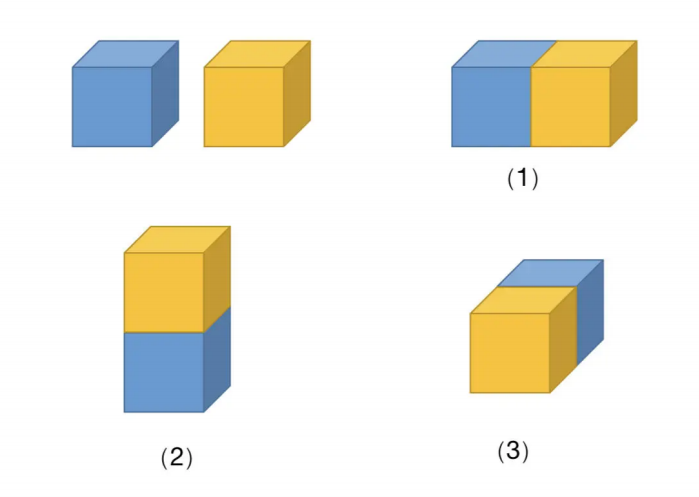
\includegraphics[scale=.3]{part/人工智能/深度学习框架/pic/Pytorch/Pytorch基础/cat的拼接方式.png}
\caption{cat的拼接方式}
\end{minipage}
\hspace{0.05\textwidth} % 调整这里的参数来改变图片之间的空隙
\begin{minipage}[t]{0.45\textwidth}
\centering
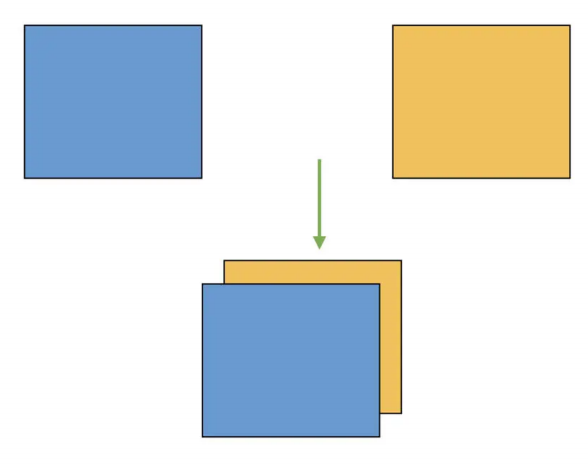
\includegraphics[scale=.3]{part/人工智能/深度学习框架/pic/Pytorch/Pytorch基础/stack的拼接方式.png}
\caption{stack的拼接方式}
\end{minipage}
\caption{cat和stack的拼接方式}
\end{figure}


\codeinline{cat} 实际上是将多个 Tensor 在已有的维度上进行连接，

\subsubsection{stack() 增加维度连接}
\label{subsubsec:Pytorch的stack()函数}
那如果想增加新的维度进行连接，这时候就需要 \codeinline{stack} 函数登场了。
\begin{lstlisting}[style=demostyle,numbers=none]
# stack() 用于连接张量
torch.stack(tensors, dim=0, out=None)
# tensors: 张量序列
# dim: 沿着哪个维度拼接
# out: 输出张量
\end{lstlisting}
\begin{lstlisting}[style=pythonstyle]
import torch

# 两个二维张量
A=torch.ones(3,3)
B=2*torch.ones(3,3)

print("A.size():",A.size())
print("B.size():",B.size())

print("torch.stack((A,B),0).size():",torch.stack((A,B),0).size())
print("torch.stack((A,B),1).size():",torch.stack((A,B),1).size())
print("torch.stack((A,B),2).size():",torch.stack((A,B),2).size())
\end{lstlisting}

\begin{lstlisting}[style=demostyle,numbers=none]
A.size(): torch.Size([3, 3])
B.size(): torch.Size([3, 3])
torch.stack((A,B),0).size(): torch.Size([2, 3, 3])
torch.stack((A,B),1).size(): torch.Size([3, 2, 3])
torch.stack((A,B),2).size(): torch.Size([3, 3, 2])
\end{lstlisting}

\begin{derivation}{推导stack的拼接方式}
    \begin{enumerate}[label=\arabic*)]
        \item 维度0

        对于A的维度0就是第0个括号开始的
        \begin{lstlisting}[style=demostyle,numbers=none]
            [[1., 1., 1.],
             [1., 1., 1.],
             [1., 1., 1.]]
        \end{lstlisting}   
            
        同理B的维度0就是第0个括号开始的
        \begin{lstlisting}[style=demostyle,numbers=none]
            [[2., 2., 2.],
             [2., 2., 2.],
             [2., 2., 2.]]
        \end{lstlisting}

        在维度0上拼接就是将A和B在维度0上合并(新增第0个[]括号)
        \begin{lstlisting}[style=demostyle,numbers=none]
        [ # 新增的维度0
            [[1., 1., 1.],
             [1., 1., 1.],
             [1., 1., 1.]],

            [[2., 2., 2.],
             [2., 2., 2.],
             [2., 2., 2.]]
        ]
        \end{lstlisting}

        \item 维度1

        对于A的维度0就是第1个括号开始的
        \begin{lstlisting}[style=demostyle,numbers=none]
        [   # 这层括号不看了
            [1., 1., 1.],
            [1., 1., 1.],
            [1., 1., 1.]
        ]   # 这层括号不看了
        \end{lstlisting}

        同理B的维度0就是第1个括号开始的
        \begin{lstlisting}[style=demostyle,numbers=none]
        [   # 这层括号不看了
            [2., 2., 2.],
            [2., 2., 2.],
            [2., 2., 2.]
        ]   # 这层括号不看了
        \end{lstlisting}

        在维度1上拼接就是将A和B在维度0上合并(新增第1个[]括号)
        \begin{lstlisting}[style=demostyle,numbers=none]
        [
            [ # 新增第1个[]括号
             [1., 1., 1.],
             [2., 2., 2.]
            ],
   
            [
             [1., 1., 1.],
             [2., 2., 2.]
            ],
   
           [
             [1., 1., 1.],
             [2., 2., 2.]
            ]
        ]
        \end{lstlisting}

        \item 维度2

        对于A的维度0就是第2个括号开始的
        \begin{lstlisting}[style=demostyle,numbers=none]
        [   # 这层括号不看了
            [# 这层括号不看了
                1.,
                1., 
                1.
            ],

            [# 这层括号不看了
                1., 
                1., 
                1.
            ],

            [# 这层括号不看了
                1., 
                1., 
                1.
            ]
        ]   # 这层括号不看了
    \end{lstlisting}

    同理B的维度0就是第2个括号开始的
    \begin{lstlisting}[style=demostyle,numbers=none]
    [   # 这层括号不看了
        [# 这层括号不看了
            2.,
            2., 
            2.
        ],

        [# 这层括号不看了
            2., 
            2., 
            2.
        ],

        [# 这层括号不看了
            2., 
            2., 
            2.
        ]
    ]   # 这层括号不看了
    \end{lstlisting}

    在维度2上拼接就是将A和B在维度0上合并(新增第2个[]括号)
    \begin{lstlisting}[style=demostyle,numbers=none]
    [
        [ 
            [1., 2.], # 新增第2个[]括号
            [1., 2.],
            [1., 2.]
        ],

        [
            [1., 2.],
            [1., 2.],
            [1., 2.]
        ],

        [
            [1., 2.],
            [1., 2.],
            [1., 2.]
        ]
    ]
    \end{lstlisting}

    \end{enumerate}
    
\end{derivation}

详细展开发现

\begin{lstlisting}[style=demostyle,numbers=none]
>>> A=torch.ones(3,3)
>>> B=2*torch.ones(3,3)
>>> A
tensor([[1., 1., 1.],
        [1., 1., 1.],
        [1., 1., 1.]])
>>> B
tensor([[2., 2., 2.],
        [2., 2., 2.],
        [2., 2., 2.]])
>>> torch.stack((A,B),0)
tensor([[[1., 1., 1.],
         [1., 1., 1.],
         [1., 1., 1.]],

        [[2., 2., 2.],
         [2., 2., 2.],
         [2., 2., 2.]]])
>>> torch.stack((A,B),1)
tensor([[[1., 1., 1.],
         [2., 2., 2.]],

        [[1., 1., 1.],
         [2., 2., 2.]],

        [[1., 1., 1.],
         [2., 2., 2.]]])
>>> torch.stack((A,B),2)
tensor([[[1., 2.],
         [1., 2.],
         [1., 2.]],

        [[1., 2.],
         [1., 2.],
         [1., 2.]],

        [[1., 2.],
         [1., 2.],
         [1., 2.]]])
\end{lstlisting}      



\begin{lstlisting}[style=demostyle,numbers=none]
>>> A=torch.arange(0,4)
tensor([0, 1, 2, 3])
>>> B=torch.arange(5,9)
>>> B
tensor([5, 6, 7, 8])

>>> C=torch.stack((A,B),0)
>>> C
tensor([[0, 1, 2, 3],
        [5, 6, 7, 8]])
>>> D=torch.stack((A,B),1)
>>> D
tensor([[0, 5],
        [1, 6],
        [2, 7],
        [3, 8]])
\end{lstlisting}

\subsection{Tensor的切片}
\label{subsec:Pytorch的Tensor的切片}
切分就是连接的逆过程，有了刚才的经验

PyTorch 中的 Tensor 支持切片操作，但是切片操作会返回一个新的 Tensor，
所以切片操作不会改变原来的 Tensor。

PyTorch提供了\codeinline{chunk()}、\codeinline{split()}和\codeinline{unbind()}函数来实现切片操作。

\subsubsection{chunk() 均分}
\label{subsubsec:Pytorch的chunk()函数}
\begin{lstlisting}[style=demostyle,numbers=none]
# chunk() 按照声明的 dim，进行尽可能平均的划分。
# 如果不能整除，则最后一个张量的维度会小于其他张量

torch.chunk(tensor, chunks, dim=0)
# tensor: 输入张量
# chunks: 切分后的块数
# dim: 切分维度
\end{lstlisting}
\begin{lstlisting}[style=pythonstyle]
import torch

# 示例1：一维张量的均分
A = torch.tensor([1, 2, 3, 4, 5, 6, 7, 8, 9, 10])

# 将A沿着dim=0方向均分为2个块
B = torch.chunk(A, 2, 0)
print("示例1：一维张量的均分")
for i, chunk in enumerate(B):
    print(f"块{i+1}:", chunk)

# 示例2：一维张量不能均分的情况
# 将A沿着dim=0方向分成3个块，不能整除的情况下最后一个块包含剩余元素
C = torch.chunk(A, 3, 0)
print("\n示例2：一维张量不能均分的情况")
for i, chunk in enumerate(C):
    print(f"块{i+1}:", chunk)

# 示例3：二维张量的分块
D = torch.tensor([[1, 2, 3], [4, 5, 6], [7, 8, 9], [10, 11, 12]])

# 将D沿着dim=0（行方向）分成2个块
E = torch.chunk(D, 2, 0)
print("\n示例3：二维张量沿行方向的均分")
for i, chunk in enumerate(E):
    print(f"块{i+1}:\n", chunk)

# 将D沿着dim=1（列方向）分成2个块
# chunk 函数是先做除法，然后再向上取整得到每组的数量。
F = torch.chunk(D, 2, 1)
print("\n示例4：二维张量沿列方向的均分")
for i, chunk in enumerate(F):
    print(f"块{i+1}:\n", chunk)

# 示例5：如果 chunk 参数大于 Tensor 可以切分的长度
# 将D沿着dim=1（列方向）分成4个块，不均分时，最后一个块包含剩余的元素
G = torch.chunk(D, 4, 1)
print("\n示例5：二维张量沿列方向不能均分的情况")
for i, chunk in enumerate(G):
    print(f"块{i+1}:\n", chunk)

# 示例6：三维张量的分块
H = torch.tensor([[[1, 2], [3, 4]], [[5, 6], [7, 8]], [[9, 10], [11, 12]]])

# 将H沿着dim=0（最外层维度）分成3个块
I = torch.chunk(H, 3, 0)
print("\n示例6：三维张量沿最外层维度的均分")
for i, chunk in enumerate(I):
    print(f"块{i+1}:\n", chunk)
\end{lstlisting}
\begin{lstlisting}[style=demostyle,numbers=none]
示例1：一维张量的均分
块1: tensor([1, 2, 3, 4, 5])
块2: tensor([ 6,  7,  8,  9, 10])

示例2：一维张量不能均分的情况
块1: tensor([1, 2, 3, 4])
块2: tensor([5, 6, 7, 8])
块3: tensor([ 9, 10])

示例3：二维张量沿行方向的均分
块1:
tensor([[1, 2, 3],
        [4, 5, 6]])
块2:
tensor([[ 7,  8,  9],
        [10, 11, 12]])

示例4：二维张量沿列方向的均分
块1:
tensor([[ 1,  2],
        [ 4,  5],
        [ 7,  8],
        [10, 11]])
块2:
tensor([[ 3],
        [ 6],
        [ 9],
        [12]])

示例5：如果 chunk 参数大于 Tensor 可以切分的长度
块1:
tensor([[ 1],
        [ 4],
        [ 7],
        [10]])
块2:
tensor([[ 2],
        [ 5],
        [ 8],
        [11]])
块3:
tensor([[ 3],
        [ 6],
        [ 9],
        [12]])

示例6：三维张量沿最外层维度的均分
块1:
tensor([[[1, 2],
        [3, 4]]])
块2:
tensor([[[5, 6],
        [7, 8]]])
块3:
tensor([[[ 9, 10],
        [11, 12]]])
\end{lstlisting}

\subsubsection{split() 按照指定大小切分}
\label{subsubsec:Pytorch的split()函数}
\begin{lstlisting}[style=demostyle,numbers=none]
# split() 按照声明的 dim，进行划分。
torch.split(tensor, split_size_or_sections, dim=0)
# split_size_or_sections 这个参数。
#   当它为整数时，表示将 tensor 按照每块大小为这个整数的数值来切割；
#   当这个参数为列表时，则表示将此 tensor 切成和列表中元素一样大小的块。
# 
#   如果使用list,要保证 list的和等于 改维度的大小
\end{lstlisting}
\begin{lstlisting}[style=pythonstyle]
import torch

# 示例1：一维张量，按照固定大小分割l
A = torch.tensor([1, 2, 3, 4, 5, 6, 7, 8, 9, 10])

# 将A按照每块大小为3进行分割，dim=0（默认）
B = torch.split(A, 3, 0)
print("示例1：一维张量，按照固定大小分割")
for i, chunk in enumerate(B):
    print(f"块{i+1}:", chunk)

# 示例2：一维张量，不能均分的情况
# 将A按照每块大小为4进行分割，最后一个块包含剩余元素
C = torch.split(A, 4, 0)
print("\n示例2：一维张量，不能均分的情况")
for i, chunk in enumerate(C):
    print(f"块{i+1}:", chunk)

# 示例3：一维张量，按照列表分割
# 将A按照列表[2, 3, 5]指定的块大小进行分割
# 
# 这里第0维度一共10个元素，因此 list 中的元素之和应该等于 10=2+3+5
D = torch.split(A, [2, 3, 5], 0)
print("\n示例3：一维张量，按照列表分割")
for i, chunk in enumerate(D):
    print(f"块{i+1}:", chunk)

# 示例4：二维张量，按行分割
E = torch.tensor([[1, 2, 3], [4, 5, 6], [7, 8, 9], [10, 11, 12]])

# 将E沿着dim=0（行方向）按照每块大小为2进行分割
F = torch.split(E, 2, 0)
print("\n示例4：二维张量，按行分割")
for i, chunk in enumerate(F):
    print(f"块{i+1}:\n", chunk)

# 示例5：二维张量，按列分割
# 将E沿着dim=1（列方向）按照每块大小为2进行分割
G = torch.split(E, 2, 1)
print("\n示例5：二维张量，按列分割")
for i, chunk in enumerate(G):
    print(f"块{i+1}:\n", chunk)

# 示例6：二维张量，不能均分的情况
# 将E沿着dim=1（列方向）分成[1, 2]两块
H = torch.split(E, [1, 2], 1)
print("\n示例6：二维张量，不能均分的情况")
for i, chunk in enumerate(H):
    print(f"块{i+1}:\n", chunk)

# 示例7：三维张量，按最外层维度分割
I = torch.tensor([[[1, 2], [3, 4]], [[5, 6], [7, 8]], [[9, 10], [11, 12]]])

# 将I沿着dim=0分割成每块大小为1的块
J = torch.split(I, 1, 0)
print("\n示例7：三维张量，按最外层维度分割")
for i, chunk in enumerate(J):
    print(f"块{i+1}:\n", chunk)

# 示例8：三维张量，按第二维度分割
# 将I沿着dim=1（第二维度）分割成每块大小为1的块
K = torch.split(I, 1, 1)
print("\n示例8：三维张量，按第二维度分割")
for i, chunk in enumerate(K):
    print(f"块{i+1}:\n", chunk)
\end{lstlisting}
\begin{lstlisting}[style=demostyle,numbers=none]
示例1：一维张量，按照固定大小分割
块1: tensor([1, 2, 3])
块2: tensor([4, 5, 6])
块3: tensor([7, 8, 9])
块4: tensor([10])

示例2：一维张量，不能均分的情况
块1: tensor([1, 2, 3, 4])
块2: tensor([5, 6, 7, 8])
块3: tensor([ 9, 10])

示例3：一维张量，按照列表分割
块1: tensor([1, 2])
块2: tensor([3, 4, 5])
块3: tensor([ 6,  7,  8,  9, 10])

示例4：二维张量，按行分割
块1:
tensor([[1, 2, 3],
        [4, 5, 6]])
块2:
tensor([[ 7,  8,  9],
        [10, 11, 12]])

示例5：二维张量，按列分割
块1:
tensor([[ 1,  2],
        [ 4,  5],
        [ 7,  8],
        [10, 11]])
块2:
tensor([[ 3],
        [ 6],
        [ 9],
        [12]])

示例6：二维张量，不能均分的情况
块1:
tensor([[ 1],
        [ 4],
        [ 7],
        [10]])
块2:
tensor([[ 2,  3],
        [ 5,  6],
        [ 8,  9],
        [11, 12]])

示例7：三维张量，按最外层维度分割
块1:
tensor([[[1, 2],
        [3, 4]]])
块2:
tensor([[[5, 6],
        [7, 8]]])
块3:
tensor([[[ 9, 10],
        [11, 12]]])

示例8：三维张量，按第二维度分割
块1:
tensor([[[ 1,  2]],

        [[ 5,  6]],

        [[ 9, 10]]])
块2:
tensor([[[ 3,  4]],

        [[ 7,  8]],

        [[11, 12]]])
\end{lstlisting}

\subsubsection{unbind() 按照指定维度切分}
\label{subsubsec:Pytorch的unbind()}
如果我们现在有一个 3 channel 图像的 Tensor，想要逐个获取每个 channel 的数据,
假如用 \codeinline{chunk} 的话，我们需要将 \codeinline{chunks} 设为 3；
如果用 \codeinline{split} 的话，需要将 \codeinline{split\_size\_or\_sections} 设为 1.

虽然它们都可以实现相同的目的，但是如果 channel 数量很大，逐个去取也比较折腾。
这时候，就需要用到另一个函数：\codeinline{unbind}，它的函数定义如下
\begin{lstlisting}[style=demostyle,numbers=none]
# unbind() 按照声明的 dim，进行切分。
torch.unbind(tensor, dim=0)
\end{lstlisting}

\begin{lstlisting}[style=pythonstyle]
import torch

# 示例1：三通道图像的三维张量，按第一个维度分割
# 假设我们有一个三通道的图像张量，大小为 (3, 4, 4)
image_tensor = torch.tensor([
    [[1, 2, 3, 4], [5, 6, 7, 8], [9, 10, 11, 12], [13, 14, 15, 16]],    # 第一个通道
    [[17, 18, 19, 20], [21, 22, 23, 24], [25, 26, 27, 28], [29, 30, 31, 32]], # 第二个通道
    [[33, 34, 35, 36], [37, 38, 39, 40], [41, 42, 43, 44], [45, 46, 47, 48]]  # 第三个通道
])

# 使用unbind方法按dim=0分割（将每个通道分开）
channels = torch.unbind(image_tensor, dim=0)
print("示例1：三通道图像张量按dim=0分割")
for i, channel in enumerate(channels):
    print(f"通道{i+1}:\n", channel)

# 示例2：二维张量，按行分割
tensor_2d = torch.tensor([[1, 2, 3], [4, 5, 6], [7, 8, 9]])

# 使用unbind方法按dim=0分割（按行分割）
rows = torch.unbind(tensor_2d, dim=0)
print("\n示例2：二维张量按行分割")
for i, row in enumerate(rows):
    print(f"行{i+1}:", row)

# 使用unbind方法按dim=1分割（按列分割）
cols = torch.unbind(tensor_2d, dim=1)
print("\n示例3：二维张量按列分割")
for i, col in enumerate(cols):
    print(f"列{i+1}:", col)

# 示例4：三维张量，按第二维度分割
tensor_3d = torch.tensor([
    [[1, 2], [3, 4], [5, 6]],
    [[7, 8], [9, 10], [11, 12]]
])

# 使用unbind方法按dim=1分割（按第二维度分割，即分割每个二维张量）
split_second_dim = torch.unbind(tensor_3d, dim=1)
print("\n示例4：三维张量按第二维度分割")
for i, sub_tensor in enumerate(split_second_dim):
    print(f"分块{i+1}:\n", sub_tensor)

# 示例5：四维张量，按第三维度分割
tensor_4d = torch.tensor([
    [[[1], [2]], [[3], [4]]],
    [[[5], [6]], [[7], [8]]]
])

# 使用unbind方法按dim=2分割（按第三维度分割）
split_third_dim = torch.unbind(tensor_4d, dim=2)
print("\n示例5：四维张量按第三维度分割")
for i, sub_tensor in enumerate(split_third_dim):
    print(f"分块{i+1}:\n", sub_tensor)
\end{lstlisting}
\begin{lstlisting}[style=demostyle,numbers=none]
示例1：三通道图像张量按dim=0分割
通道1:
    tensor([[ 1,  2,  3,  4],
        [ 5,  6,  7,  8],
        [ 9, 10, 11, 12],
        [13, 14, 15, 16]])
通道2:
    tensor([[17, 18, 19, 20],
        [21, 22, 23, 24],
        [25, 26, 27, 28],
        [29, 30, 31, 32]])
通道3:
    tensor([[33, 34, 35, 36],
        [37, 38, 39, 40],
        [41, 42, 43, 44],
        [45, 46, 47, 48]])

示例2：二维张量按行分割
行1: tensor([1, 2, 3])
行2: tensor([4, 5, 6])
行3: tensor([7, 8, 9])

示例3：二维张量按列分割
列1: tensor([1, 4, 7])
列2: tensor([2, 5, 8])
列3: tensor([3, 6, 9])

示例4：三维张量按第二维度分割
分块1:
    tensor([[1, 2],
        [7, 8]])
分块2:
    tensor([[ 3,  4],
        [ 9, 10]])
分块3:
    tensor([[ 5,  6],
        [11, 12]])

示例5：四维张量按第三维度分割
分块1:
    tensor([[[1],
            [3]],

        [[5],
            [7]]])
分块2:
    tensor([[[2],
            [4]],

        [[6],
            [8]]])
\end{lstlisting}

\subsection{根据操作张量中的元素分类}
\label{subsec:Pytorch的根据操作张量中的元素分类}
\subsubsection{逐元素操作}
\label{subsec:Pytorch逐元素操作}
如表 \ref{tab:Pytorch逐元素操作} 所示，PyTorch 提供了很多逐元素操作的函数，可以对张量进行逐元素操作。
\begin{table}[h]
\centering
\begin{tabular}{|l|l|}
\hline
\textbf{函数} & \textbf{说明} \\ \hline
\codeinline{abs/add} & 绝对值 / 加法 \\ \hline
\codeinline{addcdiv(t, t1, t2, value=1)} & \codeinline{t1} 与 \codeinline{t2} 按元素除后，乘以 \codeinline{value} 加 \codeinline{t} \\ \hline
\codeinline{addcmul(t, t1, t2, value=1)} & \codeinline{t1} 与 \codeinline{t2} 按元素乘后，乘以 \codeinline{value} 加 \codeinline{t} \\ \hline
\codeinline{ceil/floor} & 向上取整 / 向下取整 \\ \hline
\codeinline{clamp(t, min, max)} & 将张量元素限制在指定区间 \\ \hline
\codeinline{exp/log/pow} & 指数 / 对数 / 幂 \\ \hline
\codeinline{mul(*tensor) / neg} & 逐元素乘法 / 取反 \\ \hline
\codeinline{sigmoid/tanh/softmax} & 激活函数 \\ \hline
\codeinline{sign/sqrt} & 取符号 / 开根号 \\ \hline
\end{tabular}
\caption{常见的逐元素操作}
\label{tab:Pytorch逐元素操作}
\end{table}
\begin{lstlisting}[style=pythonstyle]
import torch

# Initial tensor for demonstration
t = torch.tensor([[1.0, -2.0], [3.0, -4.0]])
t1 = torch.tensor([[2.0, 2.0], [2.0, 2.0]])
t2 = torch.tensor([[1.0, -1.0], [-1.0, 1.0]])

print("Initial Tensor t:\n", t)
print("Tensor t1:\n", t1)
print("Tensor t2:\n", t2)

# 1. abs/add
abs_result = torch.abs(t)
add_result = torch.add(t, t1)
print("\nabs(t):\n", abs_result)
print("add(t, t1):\n", add_result)

# 2. addcdiv(t, t1, t2, value=1)
addcdiv_result = torch.addcdiv(t, t1, t2, value=1)
print("\naddcdiv(t, t1, t2, value=1):\n", addcdiv_result)

# 3. addcmul(t, t1, t2, value=1)
addcmul_result = torch.addcmul(t, t1, t2, value=1)
print("\naddcmul(t, t1, t2, value=1):\n", addcmul_result)

# 4. ceil/floor
ceil_result = torch.ceil(t)
floor_result = torch.floor(t)
print("\nceil(t):\n", ceil_result)
print("floor(t):\n", floor_result)

# 5. clamp(t, min, max)
clamp_result = torch.clamp(t, min=-1, max=1)
print("\nclamp(t, min=-1, max=1):\n", clamp_result)

# 6. exp/log/pow
exp_result = torch.exp(t)
log_result = torch.log(torch.abs(t) + 1)  # Add 1 to avoid log(0)
pow_result = torch.pow(t, 2)
print("\nexp(t):\n", exp_result)
print("log(abs(t) + 1):\n", log_result)
print("pow(t, 2):\n", pow_result)

# 7. mul(*tensor)/neg
mul_result = torch.mul(t, t1)
neg_result = torch.neg(t)
print("\nmul(t, t1):\n", mul_result)
print("neg(t):\n", neg_result)

# 8. sigmoid/tanh/softmax
sigmoid_result = torch.sigmoid(t)
tanh_result = torch.tanh(t)
softmax_result = torch.softmax(t, dim=0)
print("\nsigmoid(t):\n", sigmoid_result)
print("tanh(t):\n", tanh_result)
print("softmax(t, dim=0):\n", softmax_result)

# 9. sign/sqrt
sign_result = torch.sign(t)
sqrt_result = torch.sqrt(torch.abs(t))  # sqrt on abs to avoid sqrt of negative
print("\nsign(t):\n", sign_result)
print("sqrt(abs(t)):\n", sqrt_result)
\end{lstlisting}
\begin{lstlisting}[style=demostyle,numbers=none]
Initial Tensor t:
 tensor([[ 1., -2.],
        [ 3., -4.]])
Tensor t1:
 tensor([[2., 2.],
        [2., 2.]])
Tensor t2:
 tensor([[ 1., -1.],
        [-1.,  1.]])

abs(t):
 tensor([[1., 2.],
        [3., 4.]])
add(t, t1):
 tensor([[ 3.,  0.],
        [ 5., -2.]])

addcdiv(t, t1, t2, value=1):
 tensor([[ 3., -4.],
        [ 1., -2.]])

addcmul(t, t1, t2, value=1):
 tensor([[ 3., -4.],
        [ 1., -2.]])

ceil(t):
 tensor([[ 1., -2.],
        [ 3., -4.]])
floor(t):
 tensor([[ 1., -2.],
        [ 3., -4.]])

clamp(t, min=-1, max=1):
 tensor([[ 1., -1.],
        [ 1., -1.]])

exp(t):
 tensor([[2.7183e+00, 1.3534e-01],
        [2.0086e+01, 1.8316e-02]])
log(abs(t) + 1):
 tensor([[0.6931, 1.0986],
        [1.3863, 1.6094]])
pow(t, 2):
 tensor([[ 1.,  4.],
        [ 9., 16.]])

mul(t, t1):
 tensor([[ 2., -4.],
        [ 6., -8.]])
neg(t):
 tensor([[-1.,  2.],
        [-3.,  4.]])

sigmoid(t):
 tensor([[0.7311, 0.1192],
        [0.9526, 0.0180]])
tanh(t):
 tensor([[ 0.7616, -0.9640],
        [ 0.9951, -0.9993]])
softmax(t, dim=0):
 tensor([[0.1192, 0.8808],
        [0.8808, 0.1192]])

sign(t):
 tensor([[ 1., -1.],
        [ 1., -1.]])
sqrt(abs(t)):
 tensor([[1.0000, 1.4142],
        [1.7321, 2.0000]])
\end{lstlisting}
\subsubsection{in-place操作}
\label{subsec:Pytorch的in-place操作}
在 PyTorch 中，in-place 操作是指那些直接在原地修改张量内容的操作，
而不是创建新的张量。
in-place 操作通常以 \codeinline{\_} 结尾。

\begin{enumerate}[label=\arabic*)]
        \item 数学运算
        \begin{enumerate}[itemindent=1em,label=\arabic*)]
                \item \codeinline{add\_()}: 加法操作
                \item \codeinline{sub\_()}: 减法操作
                \item \codeinline{mul\_()}: 乘法操作
                \item \codeinline{div\_()}: 除法操作
                \item \codeinline{pow\_()}: 幂操作
        \end{enumerate}
    
        \item 张量变形和索引操作
        \begin{enumerate}[itemindent=1em,label=\arabic*)]
                \item \codeinline{view\_()}: 变形操作
                \item \codeinline{reshape\_()}: 变形操作
                \item \codeinline{resize\_()}: 调整张量大小
                \item \codeinline{zero\_()}: 将张量的所有元素置为 0
                \item \codeinline{fill\_()}: 用指定的值填充张量
        \end{enumerate}
    
        \item 其他操作
        \begin{enumerate}[itemindent=1em,label=\arabic*)]
                \item \codeinline{copy\_()}: 将一个张量的内容复制到另一个张量
                \item \codeinline{index\_add\_()}: 按指定的索引对张量进行加法操作
                \item \codeinline{index\_copy\_()}: 按指定的索引对张量进行复制操作
                \item \codeinline{index\_fill\_()}: 按指定的索引对张量进行填充操作
        \end{enumerate}
    
        \item 归一化操作
        \codeinline{normalize\_()}：对张量进行归一化操作
\end{enumerate}


\begin{lstlisting}[style=pythonstyle]
import torch

# 创建一个张量
x = torch.tensor([1.0, 2.0, 3.0], requires_grad=True)

# In-place 操作示例
x.add_(1.0)       # x = [2.0, 3.0, 4.0]
x.mul_(2.0)       # x = [4.0, 6.0, 8.0]
x.zero_()        # x = [0.0, 0.0, 0.0]

# 需要注意，进行 in-place 操作时，可能会导致计算图被破坏
y = x.sum()
y.backward()     # 如果x是叶子节点，可能会报错
\end{lstlisting}

\subsubsection{内存布局连续}
\label{subsec:Pytorch的内存布局连续}
\begin{enumerate}[label=\arabic*)]
    \item 连续的 Tensor（Contiguous Tensor）：如果张量的元素在内存中是按行优先（row-major order）连续存储的，则称该张量是连续的。换句话说，张量的内存布局按照其自身的存储顺序（从前到后）逐行排列，不存在任何跳跃或间隔。

    \item 不连续的 Tensor（Non-contiguous Tensor）：不连续的张量是在内存中不按行优先存储的。这通常发生在张量经过某些操作（如转置、切片等）后，其数据不再按顺序排列，而是产生了间隔或跳跃。在这种情况下，张量的数据虽然依然可以访问，但可能需要额外的内存和计算来访问这些非连续存储的数据。
\end{enumerate}

PyTorch 提供了 \codeinline{is\_contiguous()} 方法来检查张量是否是连续的，如果张量是连续的，则返回 \codeinline{True}，否则返回 \codeinline{False}。
\begin{lstlisting}[style=pythonstyle]
import torch

# 创建一个张量
x = torch.tensor([[1.0, 2.0, 3.0], [4, 5, 6]], requires_grad=True)

# 检查张量是否是连续的
is_contiguous = x.is_contiguous()
print("x 是否是连续的: ", x.is_contiguous())

# 创建一个不连续的张量
y = x.t()
print("y 是否是连续的: ", y.is_contiguous())
\end{lstlisting}
\begin{lstlisting}[style=demostyle,numbers=none]
x 是否是连续的:  True
y 是否是连续的:  False
\end{lstlisting}

导致张量不连续的原因一下的操作：
\begin{enumerate}[label=\arabic*)]
    \item 转置操作（Transpose）：

    转置操作 \codeinline{x.t()} 或 \codeinline{x.transpose(dim0, dim1)} 
    会导致张量的存储顺序改变。
    因为转置操作会交换维度，使得在内存中的数据顺序不再是行优先的。

    \item 切片（Slicing）：
    
    对张量的部分切片操作，例如 \codeinline{x[:, ::2]}，
    也可能导致不连续。因为切片操作可能会跳过一部分数据，导致数据在内存中不再按顺序排列。
    
    \item 视图操作（View）：
    
    某些视图操作，如 \codeinline{x.view(-1, 2)}，可能需要重新排列内存中的数据。如果操作需要重新安排数据，结果张量可能是非连续的。
    
    \item 拼接（Concatenation）：
    
    例如 \codeinline{torch.cat([x1, x2], dim=0)} 如果在非连续维度上拼接，也可能产生不连续的结果。
    
    \item 高维交换（Permute）：
    
    \codeinline{x.permute(dims)} 操作会重新排列张量的维度，使其不再连续。
\end{enumerate}
\begin{lstlisting}[style=pythonstyle]
import torch

# 创建一个张量
x = torch.tensor([[1.0, 2.0, 3.0], [4, 5, 6]], requires_grad=True)

# 检查张量是否是连续的
print("x 是否是连续的: ", x.is_contiguous())

# 转置操作（Transpose）
y = x.t()
print("转置后的 y 是否是连续的: ", y.is_contiguous())  # 转置操作导致不连续

# 切片操作（Slicing）
z = x[:, ::2]  # 每隔一个元素切片
print("切片后的 z 是否是连续的: ", z.is_contiguous())  # 切片操作导致不连续

# 视图操作（View）
v = x.view(-1)  # 将张量展平为一维
print("视图后的 v 是否是连续的: ", v.is_contiguous())  # 视图操作不改变内存顺序，仍然是连续的

# 拼接操作（Concatenation）
a = torch.tensor([[7.0, 8.0, 9.0], [10, 11, 12]], requires_grad=True)
w = torch.cat([x, a], dim=0)  # 沿第0维进行拼接
print("拼接后的 w 是否是连续的: ", w.is_contiguous())  # 沿着同一个维度拼接，结果是连续的

# 高维交换（Permute）
p = x.permute(1, 0)  # 交换维度
print("高维交换后的 p 是否是连续的: ", p.is_contiguous())  # 高维交换操作导致不连续

# 结果分析
# 1. 转置操作（Transpose）会导致张量不连续，因为转置改变了元素在内存中的排列顺序。
# 2. 切片操作（Slicing）可能导致不连续，特别是切片间隔（如 [::2]）操作会跳过一些数据，破坏了连续性。
# 3. 视图操作（View）在张量连续的前提下，不改变内存顺序，因此结果仍然是连续的。
# 4. 沿着同一个维度进行拼接（Concatenation）一般不会改变张量的连续性，拼接后的张量是连续的。
# 5. 高维交换（Permute）操作改变了维度顺序，从而导致不连续。

# 对比总结
# - 转置（Transpose）、切片（Slicing，尤其是步长不为1的切片）和高维交换（Permute）操作通常会导致张量变为不连续。
# - 视图操作（View）和沿着同一维度的拼接（Concatenation）不会影响连续性，只要它们不需要重新排列数据。
\end{lstlisting}
\begin{lstlisting}[style=demostyle,numbers=none]
x 是否是连续的:  True
转置后的 y 是否是连续的:  False
切片后的 z 是否是连续的:  False
视图后的 v 是否是连续的:  True
拼接后的 w 是否是连续的:  True
高维交换后的 p 是否是连续的:  False
\end{lstlisting}




\section{autograd自动求导微分}
\label{sec:Pytorch的autograd自动求导微分}
\subsection{Tensor与Variable}
\label{subsubsec:Pytorch的Tensor与Variable}
\reminder{\lefthand}{在PyTorch 0.4.0版本之后，\codeinline{Variable}已经被弃用，
\textcolor{red}{Tensor}已经整合了Variable的功能。}
虽然Variable仍可用，但Variable返回值已经是一个Tensor（原来返回值是Variable），所以今后无需再用Variable包装Tensor。
但是了解Variable的概念有助于理解PyTorch的自动求导机制。

Variable不仅能对Tensor包装，而且能记录生成Tensor的运算（这是自动求导的关键）。
\begin{lstlisting}[style=demostyle,numbers=none]
torch.autograd.Variable{
    data,           # 就是 Tensor 张量数据
    # 下面的是Tensor梯度运算的记录
    requires_grad,  # 是否需要梯度,
                    # 并不是所有的张量都需要求导，为了节省内存
                    # 只有需要求导的张量才会计算梯度
    grad,           # 对应于data的梯度，形状与data一致
    grad_fn,        # 记录创建该Tensor时用到的Function,
                    # 该Function在反向传播计算中使用
                    # 是自动求导的关键
    is_leaf         # 是否是叶子节点
                    # 为叶子结点时，反向传播结束，其梯度仍会保存，
                    # 非叶子结点的梯度被释放，以节省内存。
}
\end{lstlisting}

0.4.0版本以后，Variable并入Tensor，
可见第\pageref{subsec:Pytorch-Tensor的结构属性}页的Tensor属性。

\begin{lstlisting}[style=demostyle,numbers=none]
torch.Tensor{
    # 与数据相关
    data,           # 张量数据，多维数组，最核心的属性
    dtype,          # 张量类型
    shape,          # 张量形状
    device,         # 张量在CPU或GPU上
    # 与梯度相关
    requires_grad,  # 是否需要梯度,
                    # 并不是所有的张量都需要求导，为了节省内存
                    # 只有需要求导的张量才会计算梯度
    grad,           # 梯度
    grad_fn,        # 创建Tensor的Function,是自动求导的关键
    is_leaf         # 是否是叶子节点
}
\end{lstlisting}
神经网络中的一个重要内容就是参数学习，而参数学习离不开求导。

几乎所有机器学习算法在训练或预测时都归结为求解最优化问题，如果目标函数可导， 
那么问题变为训练函数的驻点（即一阶导数等于零的点）。自动微分也称自动求导，
算法能够计算可导函数在某点处的导数值，是反向传播算法的一般化。

\codeinline{torch.autograd}包就是用来\textcolor{YBXPurple}{自动求导的}。
autograd包为张量上所有的操作提供了自动求导功能，\codeinline{torch.Tensor}和
\codeinline{torch.Function}为autograd包的两个核心类，
它们相互连接并生成一个有向非循环图。

\subsection{自动求导要点}
\label{subsec:Pytorch的自动求导要点}
\codeinline{autograd}包为对Tensor进行自动求导，自动求导时需考虑如下事项：
\begin{enumerate}[label=\arabic*)]
    \item 创建叶子节点（leaf node）：
    通过设置 \codeinline{requires\_grad=True}，可以记录对张量的操作，以便后续利用\codeinline{backward()}进行梯度计算。

    默认情况下，\codeinline{requires\_grad} 为 False。

    \item 修改 \codeinline{requires\_grad}：
    可以通过 \codeinline{.detach()} 或使用 \codeinline{torch.no\_grad()} 方法来临时禁止梯度计算，不记录计算历史。
    这种方式通常在评估或测试模型时使用。

    历史记录包含了如何创建张量，以及对张量的操作，这些信息被保存在 \codeinline{grad\_fn} 属性中。
    
    \item 非叶子节点的梯度计算：
    通过非叶子节点计算的张量会自动赋予 \codeinline{grad\_fn} 属性，这表明该张量是通过某个操作计算得到的。
    
    \item 调用 \codeinline{backward()}：
    当对最终得到的张量调用 \codeinline{backward()} 方法时，会计算其梯度，
    并且会将梯度累加到叶子节点的 grad 属性中。
    
    \item 指定 backward() 的梯度参数：
    可以指定 \codeinline{backward()} 中的 gradient 参数，其形状应该与调用 \codeinline{backward()} 的张量维度匹配或是可广播的。
    
    \item 反向传播的计算图：
    默认情况下，计算图在反向传播后会被释放，如果需要多次进行反向传播，
    则需要在调用 \codeinline{backward()} 时将 \codeinline{retain\_graph=True}。
    
    \item 非叶子节点的梯度：
    非叶子节点的梯度在调用 \codeinline{backward()} 时会被清除。
    
    \item 禁止自动求导：
    通过 \codeinline{torch.no\_grad()} 可以暂时禁止自动求导，例如在测试或评估模型时。
\end{enumerate}

在整个过程中，PyTorch采用计算图的形式进行组织，该计算图为动态图，
它的计算图在每次前向传播时都会重新构建，这样可以避免计算图过大导致的内存占用问题。

\subsection{计算图}
\label{subsec:Pytorch的计算图}
计算图是一种有向无环图，用来表示算子与变量之间关系的\textcolor{YBXPurple}{有向无环图}。

\subsubsection{计算图的推导}
\label{subsubsec:Pytorch的计算图的推导}
\begin{derivation}{推导计算图过程}
    
    用计算图表示表达式$z = w * x + b$

    如图\ref{fig:前向传播计算图}所示，
    表达式$z = wx+b$可写成两个表示式：如果 $y = wx$,$z=y + b$。

    其中$x, w, b$为变量,是用户创建的变量，不依赖于其他变量，故又称为\textcolor{blue}{\textbf{叶子节点}}。

    为计算各叶子节点的梯度，需要把对应的张量参数\codeinline{requires\_grad}属性设置为\codeinline{True},
    这样就可自动跟踪其历史记录。$y, z$是计算得到的变量，非叶子节点，$z$为根节点。
    \codeinline{mul}和\codeinline{add}是算子（或操作或函数）。
    这些变量及算子就构成一个完整的计算过程（或正向传播过程）。

    \begin{figure}[htbp]
    \centering
    \begin{minipage}[t]{0.4\textwidth}
    \centering
    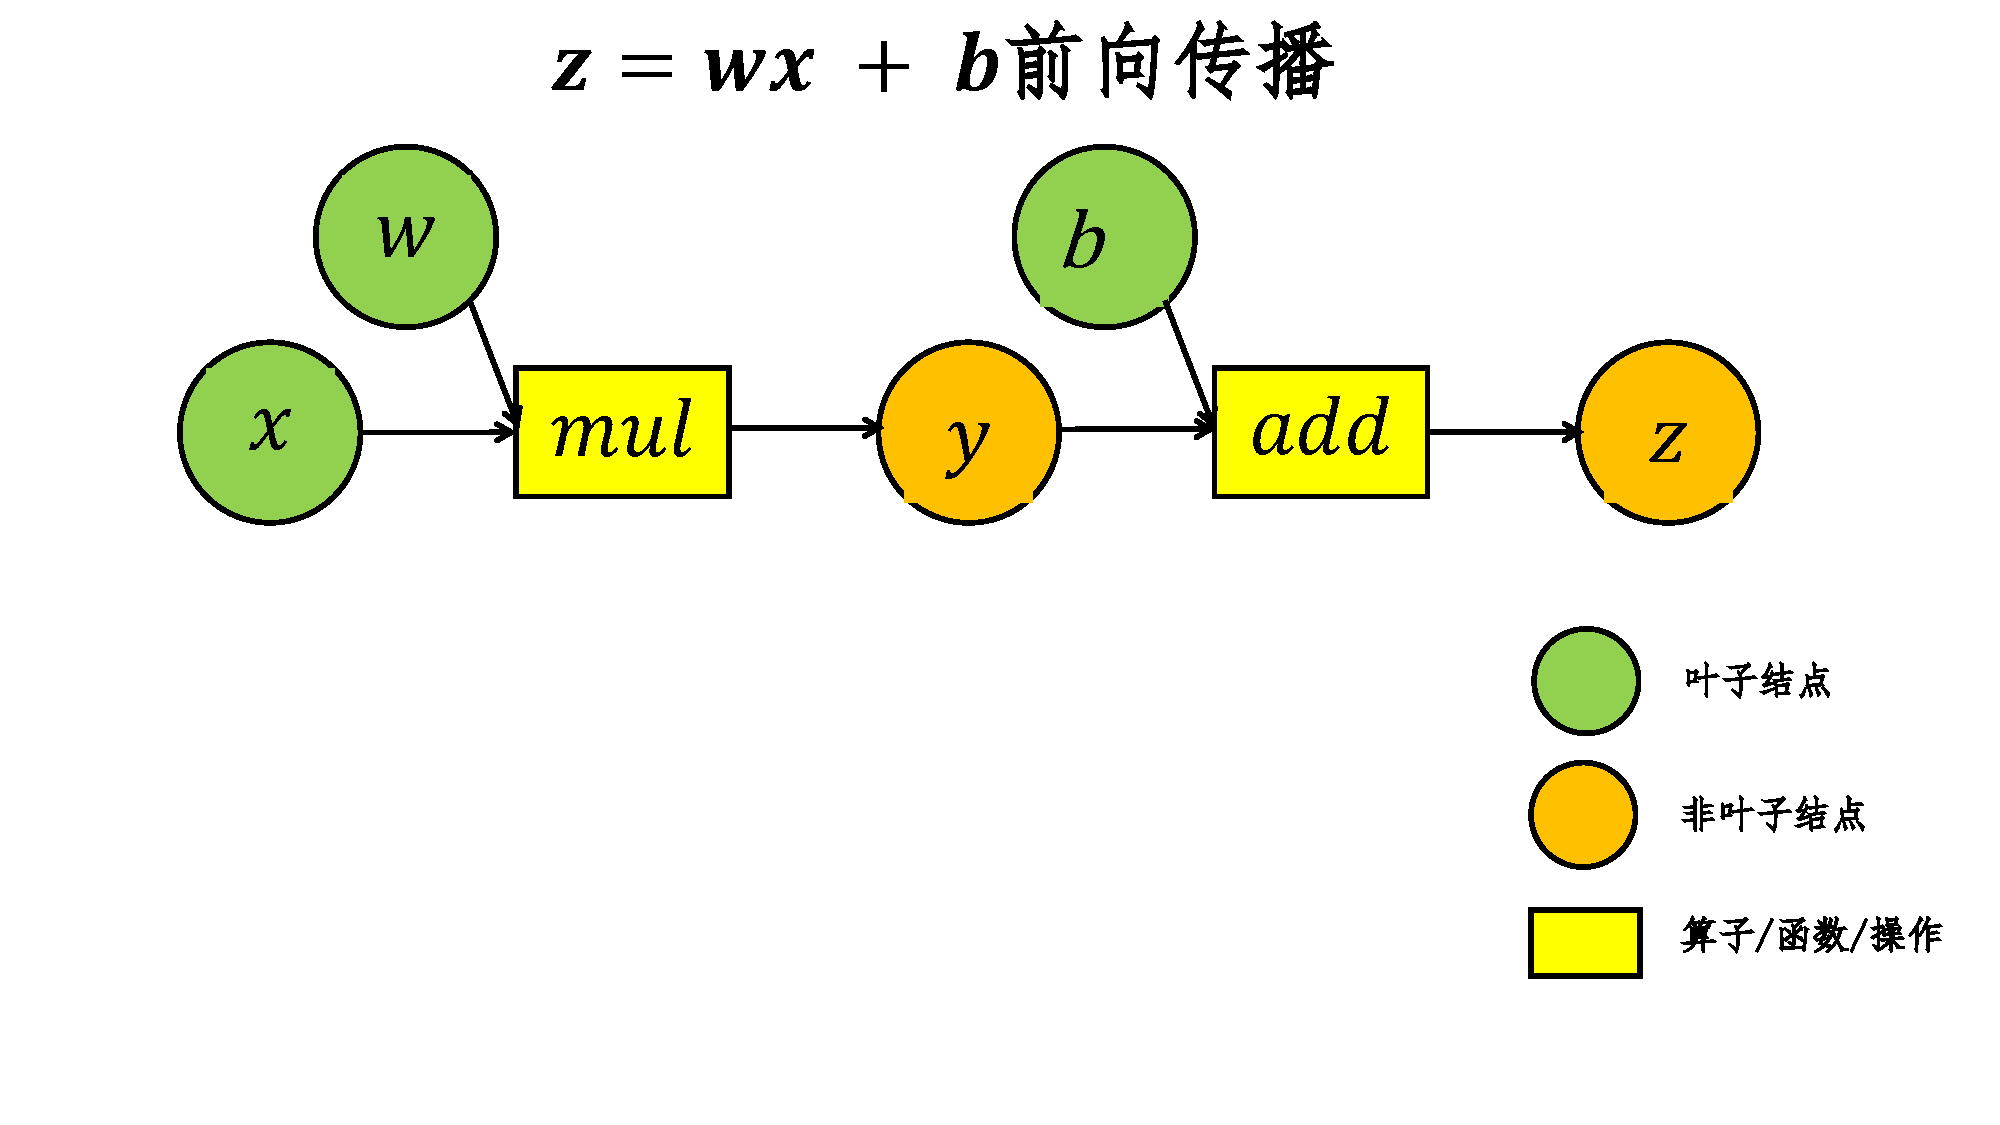
\includegraphics[width=0.5\textwidth]{part/人工智能/深度学习框架/pic/Pytorch/Pytorch基础/前向传播计算图.pdf}
    \caption{\label{fig:前向传播计算图}前向传播计算图}
    \end{minipage}
    \begin{minipage}[t]{0.4\textwidth}
    \centering
    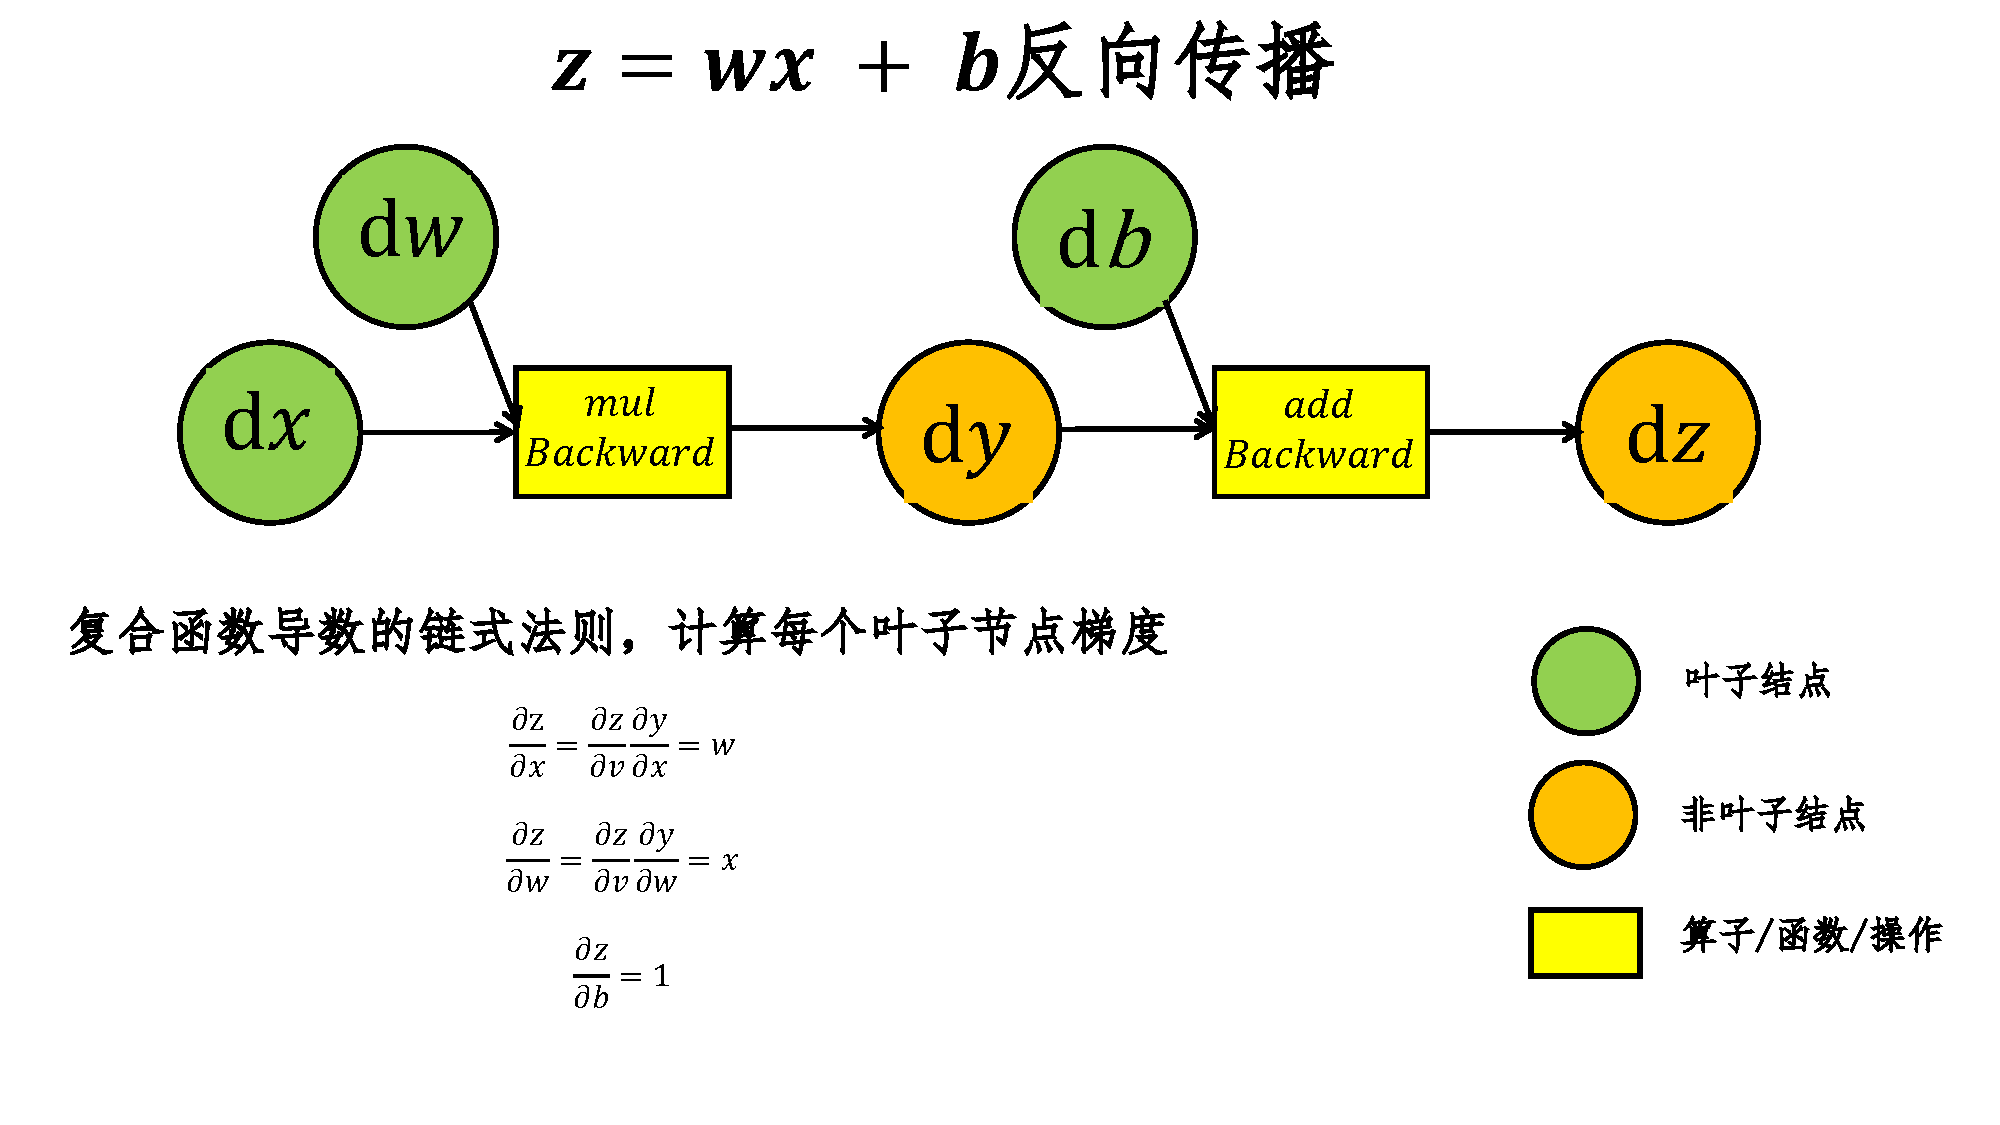
\includegraphics[width=0.5\textwidth]{part/人工智能/深度学习框架/pic/Pytorch/Pytorch基础/反向传播计算图.pdf}
    \caption{\label{fig:反向传播计算图}反向传播计算图}
    \end{minipage}
    \caption{\label{fig:前向传播和反向传播计算图}前向传播和反向传播计算图}
    \end{figure}

    图\ref{fig:反向传播计算图}所示,我们的目标是\textcolor{YBXPurple}{更新各叶子节点的梯度}，
    根据复合函数导数的链式法则，不难算出各叶子节点的梯度。

    $$\begin{aligned}
            \frac{\partial z}{\partial x}&=\frac{\partial z}{\partial y}\frac{\partial y}{\partial x}=w\\
            \frac{\partial z}{\partial w}&=\frac{\partial z}{\partial y}\frac{\partial y}{\partial w}=x\\
            \frac{\partial z}{\partial b}&=1
            \end{aligned}$$

    PyTorch调用\codeinline{backward}函数自动计算各节点的梯度，
    这是一个反向传播过程。
    在反向传播过程中，\codeinline{autograd}沿着图\ref{fig:反向传播计算图},
    从当前根节点$z$反向溯源，利用导数链式法则，计算所有叶子节点的梯度，
    并将梯度值累加到\codeinline{grad}属性中。
\end{derivation}

对非叶子节点的计算操作(或function)记录在\codeinline{grad\_fn}属性中，
叶子节点的\codeinline{grad\_fn}值为\codeinline{None}。        

PyTorch使用自动微分的计算图的生命周期如图\ref{fig:PyTorch计算图的生命周期}所示，
PyTorch中的计算图是动态计算图，
动态计算图有两个特点：
\begin{enumerate}[label=\arabic*)]
        \item 正向传播是立即执行的;
        \item 反向传播后计算图立即销毁。
\end{enumerate}

\begin{figure}[htpb]
        \centering
        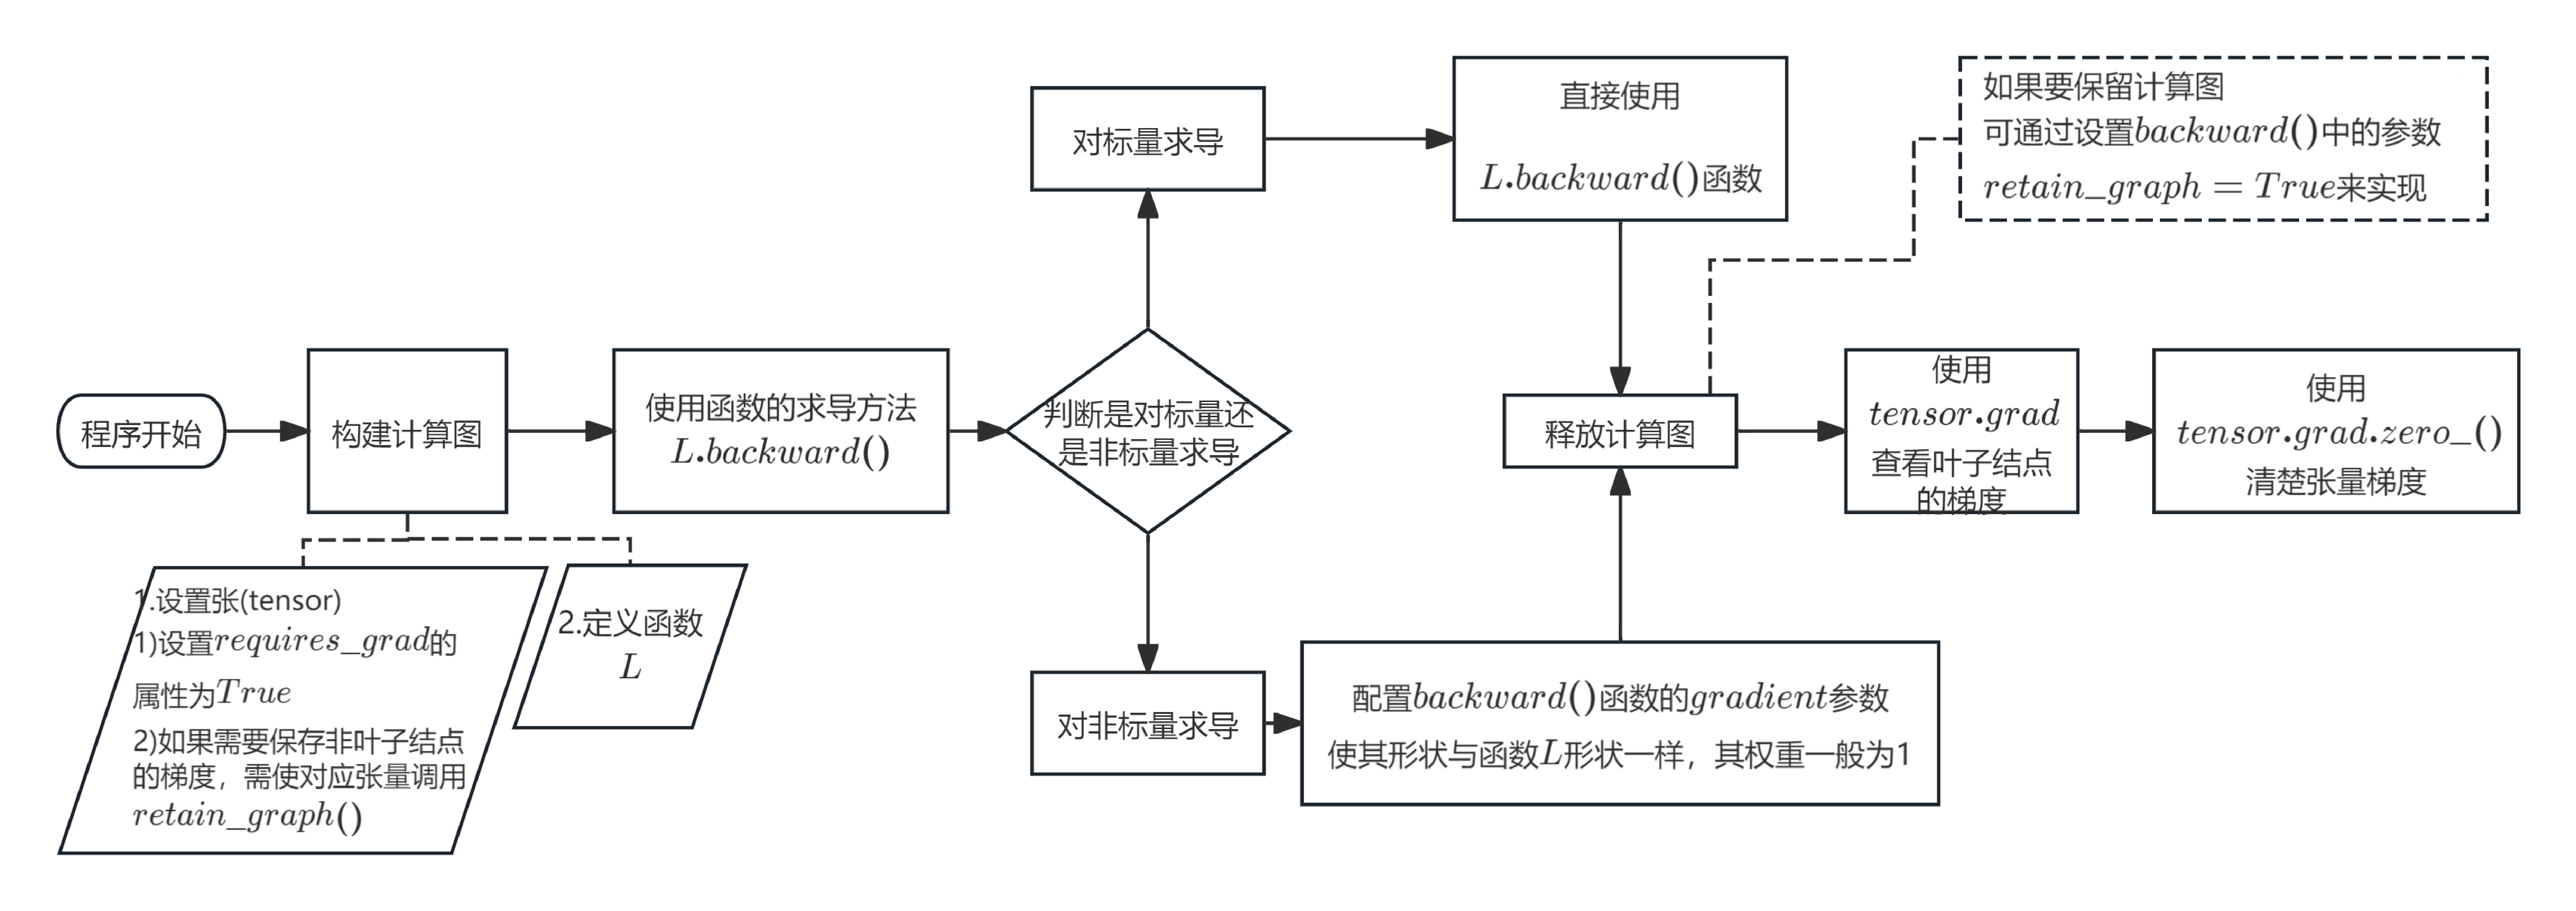
\includegraphics[width=0.8\textwidth]{part/人工智能/深度学习框架/pic/Pytorch/Pytorch基础/PyTorch计算图的生命周期.pdf}
        \caption{PyTorch计算图的生命周期}
        \label{fig:PyTorch计算图的生命周期}
\end{figure}

\begin{example}
    \exProblem
    用计算图表示 $y = (x + w) \times (w + 1)$，在$x =2, w = 1$ 时的计算图。
    \exSolution
    
    令$\left\{\begin{matrix}

        \begin{aligned}
        a &= x + w\\
        b &= w + 1\\
        y &= a \times b
        \end{aligned}
        \end{matrix}\right.$

    表示成有向无环图如图\ref{fig:计算图例题演示}所示。

    \begin{figure}[htpb]
        \centering
        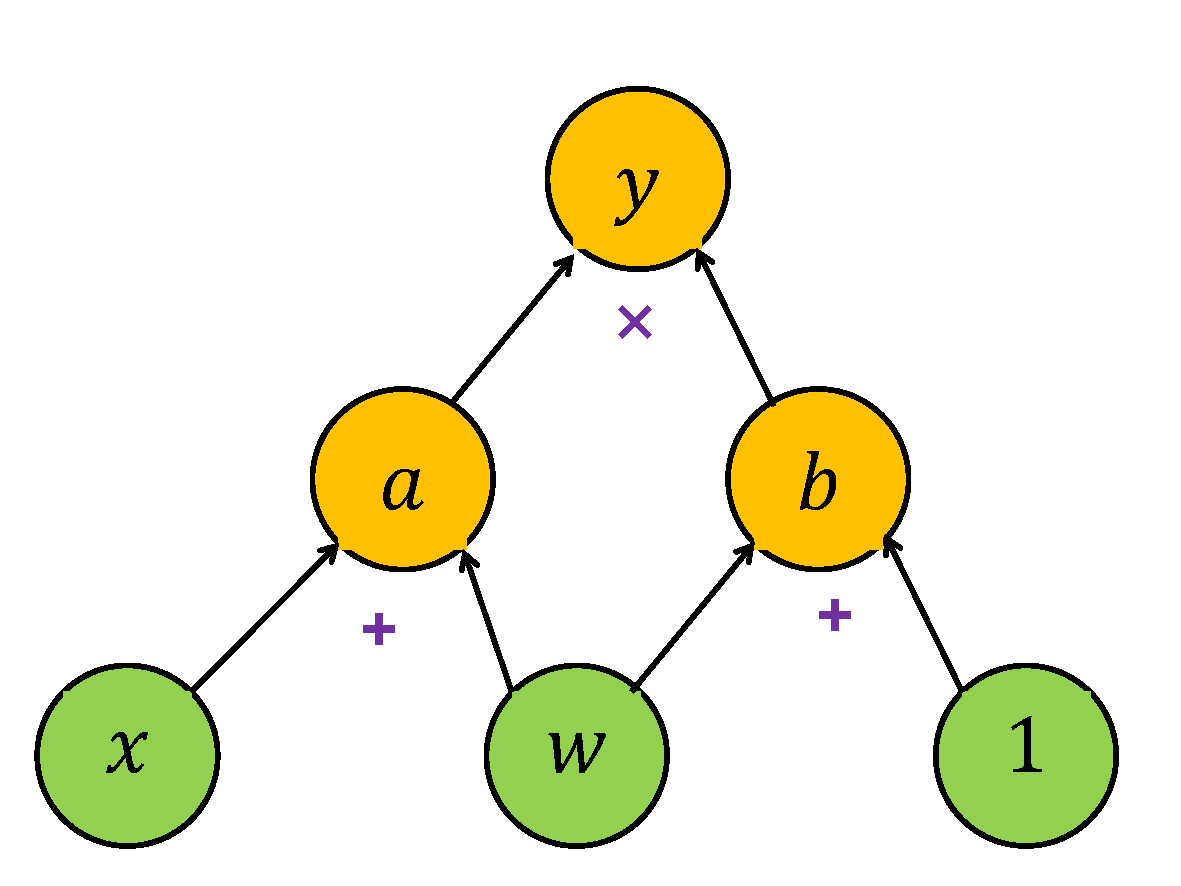
\includegraphics[width=0.4\textwidth]{part/人工智能/深度学习框架/pic/Pytorch/Pytorch基础/计算图例题演示.pdf}
        \caption{计算图例题演示}
        \label{fig:计算图例题演示}
    \end{figure}

    带入$x = 2, w = 1$，计算$y$的值，就是前向传播的过程。

    \begin{figure}[htpb]
        \centering
        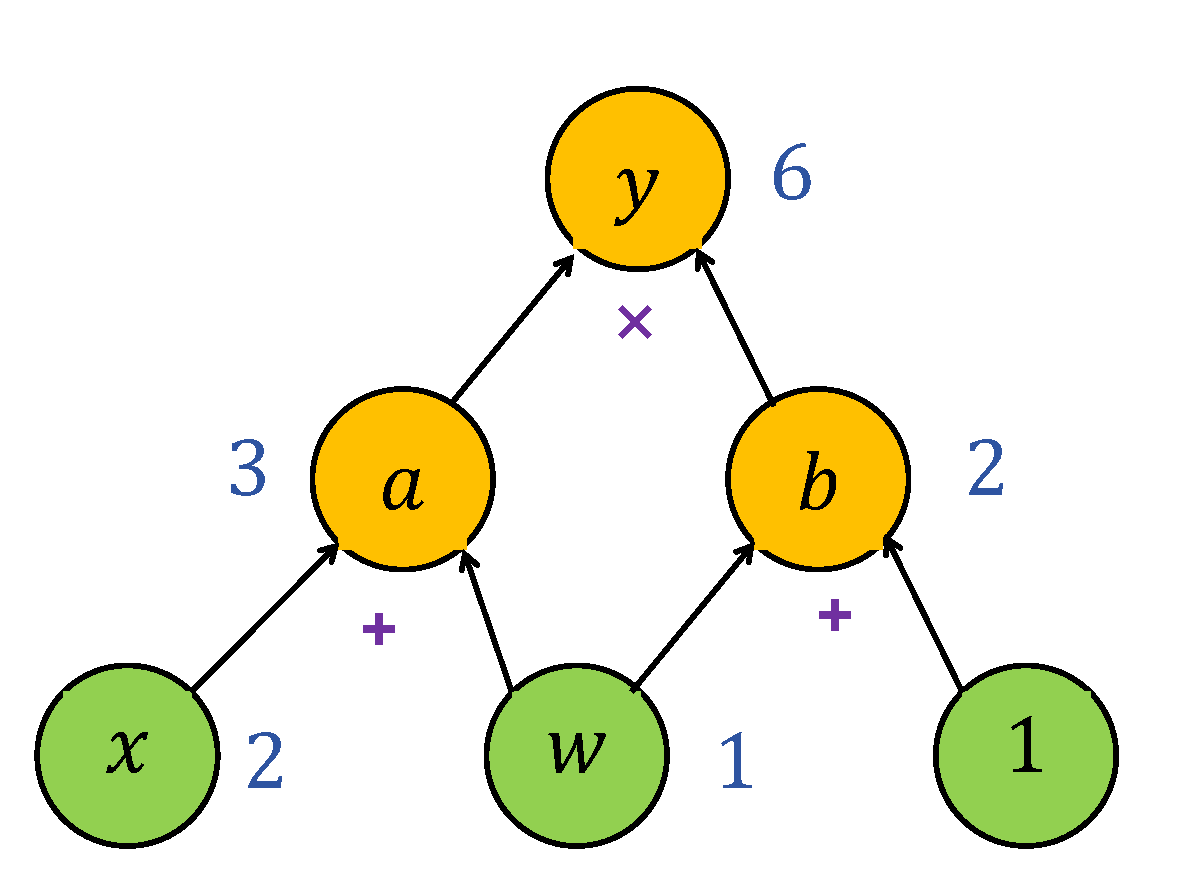
\includegraphics[width=0.4\textwidth]{part/人工智能/深度学习框架/pic/Pytorch/Pytorch基础/计算图例题演示-前向传播.pdf}
        \caption{计算图例题演示-前向传播}
        \label{fig:计算图例题演示-前向传播}
    \end{figure}

    $y$对$w$计算偏导
    $$\begin{aligned}
        \frac{\partial y}{\partial w}& = \frac{\partial y}{\partial a} \frac{\partial a}{\partial w} + \frac{\partial y}{\partial b} \frac{\partial b}{\partial w} \\
        &=b\times1+a\times1 \\
        &=b+a \\
        &= (w + 1) + (x + w) \\
        &=2*w+x+1 \\
        &=2\star1+2+1=5
        \end{aligned}$$

    \begin{figure}[htpb]
        \centering
        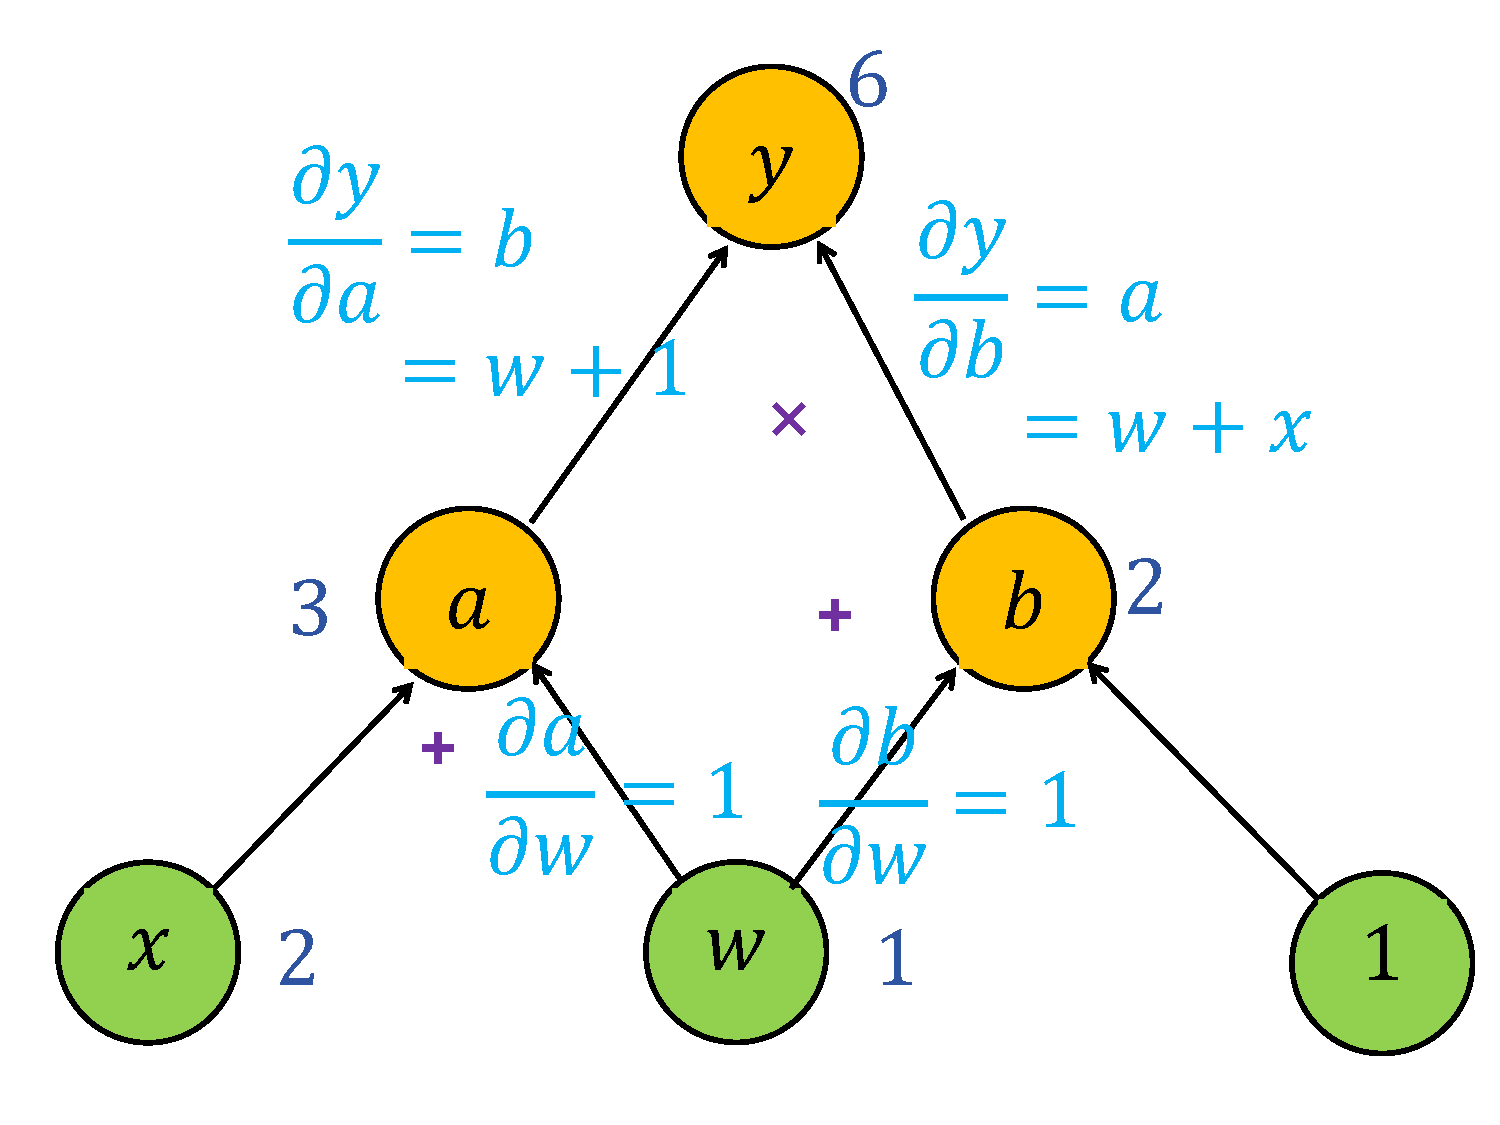
\includegraphics[width=0.4\textwidth]{part/人工智能/深度学习框架/pic/Pytorch/Pytorch基础/计算图例题演示-y对w求梯度.pdf}
        \caption{计算图例题演示-y对w求梯度}
        \label{fig:计算图例题演示-y对w求梯度}
    \end{figure}
    
    用代码实现如下：
    \begin{lstlisting}[style=pythonstyle]
    import torch

    w = torch.tensor([1.0], requires_grad=True)  # 初始化权重 w
    x = torch.tensor([2.0], requires_grad=True)  # 初始化输入 x
    
    a = torch.add(w, x)  # retain_grad() 保留梯度
    b = torch.add(w, 1)
    y = torch.mul(a, b)  # 计算 y
    
    y.backward()  # 反向传播
    print("y 对 w 的梯度：", w.grad)  # 输出 y 对 w 的梯度
    \end{lstlisting}
    \begin{lstlisting}[style=demostyle,numbers=none]
    y 对 w 的梯度： tensor([5.])
    \end{lstlisting}

    同理，$y$对$x$的梯度为
    $$\begin{aligned}
        \frac{\partial y}{\partial x}& = \frac{\partial y}{\partial a} \frac{\partial a}{\partial x} \\
        &=b\times1 \\
        &=b \\
        &=w+1 \\
        &=1+1=2
        \end{aligned}$$
    
    \begin{figure}[htpb]
        \centering
        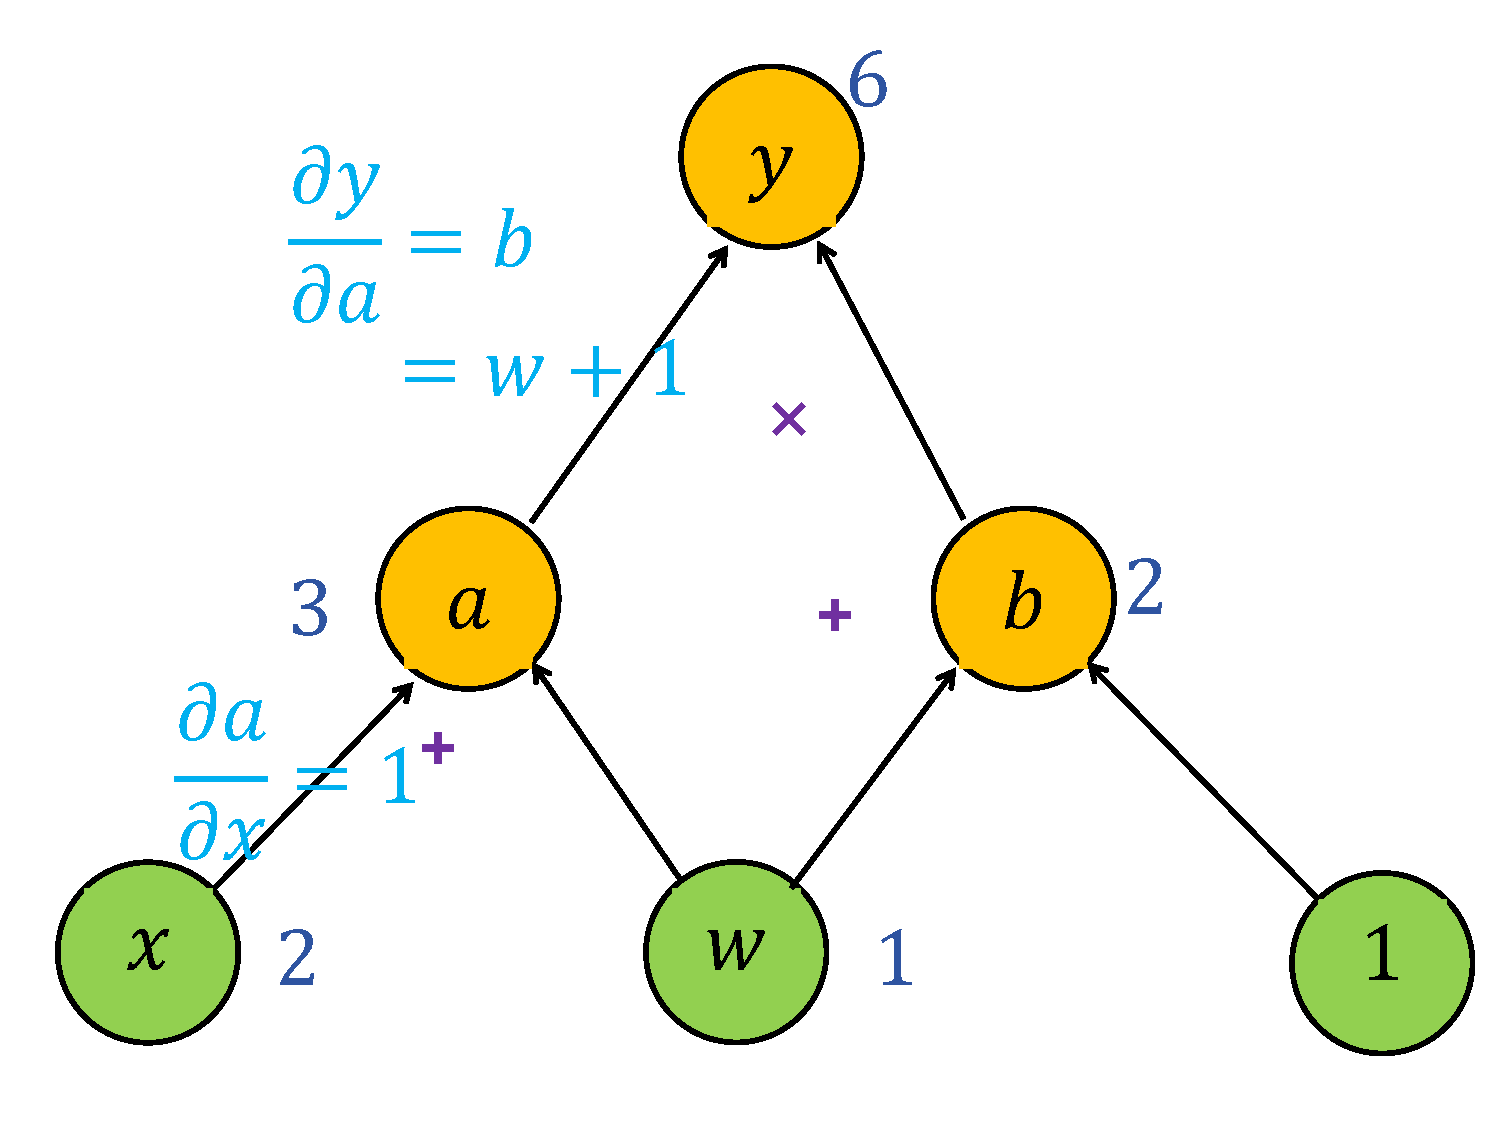
\includegraphics[width=0.4\textwidth]{part/人工智能/深度学习框架/pic/Pytorch/Pytorch基础/计算图例题演示-y对x求梯度.pdf}
        \caption{计算图例题演示-y对x求梯度}
        \label{fig:计算图例题演示-y对x求梯度}
    \end{figure}
        
    用代码实现如下：
    \begin{lstlisting}[style=pythonstyle]
    import torch

    w = torch.tensor([1.0], requires_grad=True)  # 初始化权重 w
    x = torch.tensor([2.0], requires_grad=True)  # 初始化输入 x
    
    a = torch.add(w, x)  # retain_grad() 保留梯度
    b = torch.add(w, 1)
    y = torch.mul(a, b)  # 计算 y
    
    y.backward()  # 反向传播
    print("y 对 w 的梯度：", w.grad)  # 输出 y 对 w 的梯度
    print("y 对 x 的梯度：", x.grad)  # 输出 y 对 x 的梯度
    \end{lstlisting}
    \begin{lstlisting}[style=demostyle,numbers=none]
    y 对 w 的梯度： tensor([5.])
    y 对 x 的梯度： tensor([2.])
    \end{lstlisting}
\end{example}

\subsubsection{计算图的元素}
\label{subsubsec:Pytorch的计算图的元素}
\begin{enumerate}[label=\arabic*)]
    \item 结点：

    结点表示\textcolor{YBXPurple}{数据}：向量、矩阵、张量等，
    
    结点有两种类型：
    \begin{enumerate}[itemindent=1em,label=\arabic*)]
        \item 叶子节点: 用户创建的变量，不依赖于其他变量。

        \item 非叶子节点：计算得到的变量，依赖于其他变量。
    \end{enumerate}

    只有叶子结点才有\textcolor{blue}{\textbf{梯度}}，梯度值保存在\codeinline{grad}属性中。
    \codeinline{requires\_grad}属性为\codeinline{True}。

    \begin{lstlisting}[style=pythonstyle]
    import torch

    w = torch.tensor([1.0], requires_grad=True)  # 初始化权重 w
    x = torch.tensor([2.0], requires_grad=True)  # 初始化输入 x

    a = torch.add(w, x)  # retain_grad() 保留梯度
    b = torch.add(w, 1)
    y = torch.mul(a, b)  # 计算 y

    # 查看是否是叶子节点
    print("w 是否是叶子节点：", w.is_leaf, "梯度为：", w.grad)
    print("x 是否是叶子节点：", x.is_leaf, "梯度为：", x.grad)
    print("a 是否是叶子节点：", a.is_leaf, "梯度为：", a.grad)
    print("b 是否是叶子节点：", b.is_leaf, "梯度为：", b.grad)
    print("y 是否是叶子节点：", y.is_leaf, "梯度为：", y.grad)
    \end{lstlisting}
    \begin{lstlisting}[style=demostyle,numbers=none]
    w 是否是叶子节点： True 梯度为： tensor([5.])
    x 是否是叶子节点： True 梯度为： tensor([2.])
    # 非叶子结点在反向传播结束后梯度会被自动清空
    a 是否是叶子节点： False 梯度为： None 
    b 是否是叶子节点： False 梯度为： None
    y 是否是叶子节点： False 梯度为： None
    \end{lstlisting}

    非叶子结点在反向传播结束后梯度会被自动清空。
    如果希望保留非叶子节点的梯度，可以使用\codeinline{retain\_grad()}方法。
    \begin{lstlisting}[style=pythonstyle]
    import torch

    w = torch.tensor([1.0], requires_grad=True)  # 初始化权重 w
    x = torch.tensor([2.0], requires_grad=True)  # 初始化输入 x
    
    a = torch.add(w, x)  # retain_grad() 保留梯度
    a.retain_grad()
    b = torch.add(w, 1)
    y = torch.mul(a, b)  # 计算 y
    
    y.backward()  # 反向传播
    
    
    # 查看是否是叶子节点
    print("w 是否是叶子节点：", w.is_leaf, "梯度为：", w.grad)
    print("x 是否是叶子节点：", x.is_leaf, "梯度为：", x.grad)
    print("a 是否是叶子节点：", a.is_leaf, "梯度为：", a.grad)
    print("b 是否是叶子节点：", b.is_leaf, "梯度为：", b.grad)
    print("y 是否是叶子节点：", y.is_leaf, "梯度为：", y.grad)
    \end{lstlisting}
    \begin{lstlisting}[style=demostyle,numbers=none]
    w 是否是叶子节点： True 梯度为： tensor([5.])
    x 是否是叶子节点： True 梯度为： tensor([2.])
    a 是否是叶子节点： False 梯度为： tensor([2.])
    b 是否是叶子节点： False 梯度为： None
    y 是否是叶子节点： False 梯度为： None
    \end{lstlisting}

    \item 边：

    边表示\textcolor{YBXPurple}{操作}：加法、乘法、激活函数等。
\end{enumerate}

\subsubsection{计算图的属性 grad\_fn}
\label{subsubsec:Pytorch的计算图的属性}
\codeinline{grad\_fn}属性表示该张量是通过什么操作得到的，
是一个\codeinline{Function}对象。

\codeinline{grad\_fn}的值：
\begin{enumerate}[label=\arabic*)]
    \item \textbf{None}：当一个张量是手动创建的
    
    例如使用 \codeinline{torch.tensor()} 或 \codeinline{torch.rand()}且没有参与任何需要自动求导的操作时，其 \codeinline{grad\_fn} 为 \codeinline{None}，这种张量被称为叶子节点（leaf tensor）。

    \item \textbf{AddBackward}：表示加法操作的反向传播函数。
    
    例如，\codeinline{z = x + y}，\codeinline{z.grad\_fn} 为 \codeinline{AddBackward}。

    \item \textbf{SubBackward}：表示减法操作的反向传播函数。
    
    例如，\codeinline{z = x - y}，\codeinline{z.grad\_fn} 为 \codeinline{SubBackward}。

    \item \textbf{MulBackward}：表示乘法操作的反向传播函数。
    
    例如，\codeinline{z = x * y}，\codeinline{z.grad\_fn} 为 \codeinline{MulBackward}。

    \item \textbf{DivBackward}：表示除法操作的反向传播函数。
    
    例如，\codeinline{z = x / y}，\codeinline{z.grad\_fn} 为 \codeinline{DivBackward}。

    \item \textbf{PowBackward}：表示幂运算的反向传播函数。
    
    例如，\codeinline{z = x.pow(2)}，\codeinline{z.grad\_fn} 为 \codeinline{PowBackward}。

    \item \textbf{MatMulBackward}：表示矩阵乘法操作的反向传播函数。
    
    例如，\codeinline{z = torch.matmul(x, y)} 或 \codeinline{z = x @ y}，\codeinline{z.grad\_fn} 为 \codeinline{MatMulBackward}。

    \item \textbf{MeanBackward}：表示求均值操作的反向传播函数。
    
    例如，\codeinline{z = x.mean()}，\codeinline{z.grad\_fn} 为 \codeinline{MeanBackward}。

    \item \textbf{SumBackward}：表示求和操作的反向传播函数。
    
    例如，\codeinline{z = x.sum()}，\codeinline{z.grad\_fn} 为 \codeinline{SumBackward}。

    \item \textbf{ExpBackward}：表示指数函数的反向传播函数。
    
    例如，\codeinline{z = x.exp()}，\codeinline{z.grad\_fn} 为 \codeinline{ExpBackward}。

    \item \textbf{SqrtBackward}：表示平方根函数的反向传播函数。
    
    例如，\codeinline{z = x.sqrt()}，\codeinline{z.grad\_fn} 为 \codeinline{SqrtBackward}。

    \item \textbf{LogBackward}：表示对数函数的反向传播函数。
    
    例如，\codeinline{z = x.log()}，\codeinline{z.grad\_fn} 为 \codeinline{LogBackward}。

    \item \textbf{TBackward}：表示转置操作的反向传播函数。
    
    例如，\codeinline{z = x.t()}（二维矩阵转置），\codeinline{z.grad\_fn} 为 \codeinline{TBackward}。

    \item \textbf{ReluBackward}：表示 ReLU 激活函数的反向传播函数。
    
    例如，\codeinline{z = torch.relu(x)}，\codeinline{z.grad\_fn} 为 \codeinline{ReluBackward}。

    \item \textbf{SigmoidBackward}：表示 Sigmoid 激活函数的反向传播函数。
    
    例如，\codeinline{z = torch.sigmoid(x)}，\codeinline{z.grad\_fn} 为 \codeinline{SigmoidBackward}。

    \item \textbf{ViewBackward}：表示视图操作（即张量视图转换）的反向传播函数。
    
    例如，\codeinline{z = x.view(-1)}，\codeinline{z.grad\_fn} 为 \codeinline{ViewBackward}。

    \item \textbf{CatBackward}：表示张量拼接操作的反向传播函数。
    
    例如，\codeinline{z = torch.cat((x, y), dim=0)}，\codeinline{z.grad\_fn} 为 \codeinline{CatBackward}。

    \item \textbf{CloneBackward}：表示克隆操作的反向传播函数。
    
    例如，\codeinline{z = x.clone()}，\codeinline{z.grad\_fn} 为 \codeinline{CloneBackward}。

    \item \textbf{IndexBackward}：表示索引操作的反向传播函数。
    
    例如，\codeinline{z = x[0]}，\codeinline{z.grad\_fn} 为 \codeinline{IndexBackward}。
\end{enumerate}

\begin{lstlisting}[style=pythonstyle]
import torch

w = torch.tensor([1.0], requires_grad=True)  # 初始化权重 w
x = torch.tensor([2.0], requires_grad=True)  # 初始化输入 x

a = torch.add(w, x)  # retain_grad() 保留梯度
a.retain_grad()
b = torch.add(w, 1)
y = torch.mul(a, b)  # 计算 y

y.backward()  # 反向传播


# 查看grad_fn
print("w.grad_fn: ", w.grad_fn)
print("x.grad_fn: ", x.grad_fn)
print("a.grad_fn: ", a.grad_fn)
print("b.grad_fn: ", b.grad_fn)
print("y.grad_fn: ", y.grad_fn)
\end{lstlisting}
\begin{lstlisting}[style=demostyle,numbers=none]
w.grad_fn:  None # 因为是叶子结点，所以没有grad_fn
x.grad_fn:  None
a.grad_fn:  <AddBackward0 object at 0x7fae3975ae60>
b.grad_fn:  <AddBackward0 object at 0x7fae43a57fa0>
y.grad_fn:  <MulBackward0 object at 0x7fae3975ae60>
\end{lstlisting}        

\subsection{autograd包}
\label{subsec:Pytorch的autograd包}
\subsubsection{torch.autograd 简介}
\begin{enumerate}[label=\arabic*)]
        \item 自动求导机制通过有向无环图（directed acyclic graph ，DAG）实现
        \item 在DAG中，记录数据（对应tensor.data）以及操作（对应tensor.grad\_fn）
        \item 操作在pytorch中统称为Function，
        如加法、减法、乘法、ReLU、conv、Pooling等，统统是Function  
\end{enumerate}

autograd的使用有很多方法，这里重点常用的
\begin{enumerate}[label=\arabic*)]
        \item \codeinline{torch.autograd.backward()}：自动求取梯度
        \item \codeinline{torch.autograd.grad()}：求取梯度
        \item \codeinline{torch.autograd.Function}：自定义Function
\end{enumerate}


\subsubsection{torch.autograd.backward()}
\label{subsubsec:Pytorch的torch.autograd.backward()}
PyTorch提供了\codeinline{torch.autograd.backward()}函数用于实现自动求取梯度。

\begin{lstlisting}[style=demostyle, numbers=none]
# 功能：实现自动求取梯度
torch.autograd.backward(
    tensors,                # 用于计算梯度的张量
    grad_tensors = None,    # 计算非标量的梯度。其形状一般与前面的张量保持一致。
    retain_graph=None,      # 由于PyTorch采用动态图机制,
                            # 在调用一次backward函数后PyTorch会自动销毁计算图
                            # 如果想对某个变量重复调用backward函数，则需要将该参数设置为True。
    create_graph=False,     # 创建导数计算图，用于高阶求导
                            # 当设置为True的时候可以用来计算更高阶的梯度。
    grad_variables=None     # 这个参数后面版本中应该会丢弃，直接使用grad_tensors就好了。
)  
\end{lstlisting}

\textcolor{red}{\textbf{注意}}：我们使用时候都是在张量上直接调用\codeinline{.backward()}函数，
但这里却是\codeinline{torch.autograd.backward}，为什么不一样呢？ 
其实\codeinline{Tensor.backward()}接口内部调用了\codeinline{autograd.backward}。

\begin{enumerate}[label=\arabic*)]
    \item \codeinline{retain\_grad}参数使用：
    \begin{lstlisting}[style=pythonstyle]
    #####  retain_graph=True
    import torch
    w = torch.tensor([1.], requires_grad=True)
    x = torch.tensor([2.], requires_grad=True)
    
    a = torch.add(w, x)
    b = torch.add(w, 1)
    y = torch.mul(a, b)  
    
    y.backward(retain_graph=True)
    print(w.grad)
    y.backward()
    print(w.grad) 
    \end{lstlisting} 
    \begin{lstlisting}[style=demostyle,numbers=none]
    tensor([5.])
    tensor([10.])
    \end{lstlisting}

    \begin{lstlisting}[style=pythonstyle]
    #####  retain_graph=False
    import torch
    w = torch.tensor([1.], requires_grad=True)
    x = torch.tensor([2.], requires_grad=True)

    a = torch.add(w, x)
    b = torch.add(w, 1)
    y = torch.mul(a, b)

    y.backward()
    print(w.grad)
    y.backward()
    print(w.grad)
    \end{lstlisting}
    \begin{lstlisting}[style=demostyle,numbers=none]
    tensor([5.])
    ---------------------------------------------------------------------------
    RuntimeError                              Traceback (most recent call last)
    <ipython-input-9-64bccc64184d> in <module>
        10 y.backward()
        11 print(w.grad)
    ---> 12 y.backward()
        13 print(w.grad)
    RuntimeError: Trying to backward through the graph a second time (or directly access saved tensors after they have already been freed). Saved intermediate values of the graph are freed when you call .backward() or autograd.grad(). Specify retain_graph=True if you need to backward through the graph a second time or if you need to access saved tensors after calling backward.
    \end{lstlisting}

    \item \codeinline{grad\_tensors}参数使用：
    \begin{lstlisting}[style=pythonstyle]
    w = torch.tensor([1.], requires_grad=True)
    x = torch.tensor([2.], requires_grad=True)
    
    a = torch.add(w, x)     
    b = torch.add(w, 1)
    
    y0 = torch.mul(a, b)    # y0 = (x+w) * (w+1)    dy0/dw = 2w + x + 1
    y1 = torch.add(a, b)    # y1 = (x+w) + (w+1)    dy1/dw = 2
    
    loss = torch.cat([y0, y1], dim=0)       # [y0, y1]
    
    grad_tensors = torch.tensor([1., 2.])
    
    loss.backward(gradient=grad_tensors)    # Tensor.backward中的 gradient 传入 torch.autograd.backward()中的grad_tensors
    
    # w =  1* (dy0/dw)  +   2*(dy1/dw)
    # w =  1* (2w + x + 1)  +   2*(w)
    # w =  1* (5)  +   2*(2)
    # w =  9
    
    print(w.grad)
    \end{lstlisting}
    \begin{lstlisting}[style=demostyle,numbers=none]
    tensor([9.])
    \end{lstlisting}
\end{enumerate}


\begin{example}
        \exProblem
        令$\left\{\begin{matrix}
        \begin{aligned}
        a=w+x \\
        b=w+1
        \end{aligned}
        \end{matrix}\right.$, $\left\{\begin{matrix}
        \begin{aligned}
        y_0&=a\times b = w^2+ w + wx+ x\\
        y_1&=a+b =  2w + x +1
        \end{aligned}
        \end{matrix}\right.$
        
        假定计算在$w=1, x=2$时的梯度

        当$grad f= \nabla f_{loss} = (\frac{\partial f}{\partial y_0},\frac{\partial f}{\partial y_1}) = (1,2)$,计算$w$的梯度$w.grad$

        当$\nabla f_{loss} = (3,4)$,计算$w$的梯度$w.grad$

        \exSolution
        \begin{enumerate}[label=\arabic*)]
                \item 当$\nabla f_{loss} = (1,2)$
                \begin{enumerate}[itemindent=1em,label=(\arabic*)]
                        \item 计算在$w=1, x=2$时的$y_0, y_1$的值
                        $$\left\{\begin{matrix}
                                \begin{aligned}
                                y_0=a\times b=(x+w)\times(w+1) = (2 + 1)\times(1 + 1)=6 \\
                                y_1=a+b= (x+w)+(w+1) = (2 + 1)+(1 + 1)=5 
                                \end{aligned}
                                \end{matrix}\right.
                                $$
                        \item 构造损失函数
                        因为在进行反向传播时，通常会对损失函数（loss）进行求导，以获得各个参数的梯度,因此定义函数$f_{loss}$
        
                        $$f_{loss} = f(y_0, y_1)$$
                        
                        上面的$f_{loss}$使用python实现如下
                        \begin{lstlisting}[style=pythonstyle]
                        loss = torch.cat([y_0​,y_1​],dim=0)=[6,5]
                        \end{lstlisting}
                        
                        $$\begin{aligned}
                        \frac{\partial y_0}{\partial w}&=\frac\partial{\partial w}\left[(x+w)\times(w+1)\right]\\
                        &=\frac\partial{\partial w}\left[(2+w)\times(1+w)\right] \\
                        &=(2+w)+(1+w)=3+2w 
                        \end{aligned}$$

                        当$w=1, \frac{\partial y_0}{\partial w}=3+2\times1=5$
                        
                        同理$\frac{\partial y_1}{\partial w}=\frac\partial{\partial w}\left[(x+w)+(w+1)\right]=1+1=2$

                        \item 调用\codeinline{backward()}函数计算梯度
                        当loss的梯度为$\nabla f_{loss} = (\frac{\partial\text{loss}}{\partial y_0}=1, \frac{\partial\text{loss}}{\partial y_1}=2)=(1, 2)$
        
                        上面赋值$\nabla f_{loss}$的代码如下：
                        \begin{lstlisting}[style=pythonstyle]
                        grad_tensors = torch.tensor([1., 2.])
                        loss.backward(gradient=grad_tensors)
                        \end{lstlisting}
                        
                        因此
                        $$
                        \begin{aligned}
                        w.\mathrm{grad}&=\frac{\partial\text{loss}}{\partial y_0}\times\frac{\partial y_0}{\partial w} +\frac{\partial\text{loss}}{\partial y_1}\times\frac{\partial y_1}{\partial w}\\
                        &=1\times 5 +2\times2\\
                        &=9
                        \end{aligned}
                        $$
                \end{enumerate}
                

                \item 当$\nabla f_{loss} = (3,4)$
                $$
                \begin{aligned}
                w.\mathrm{grad}&=3\times\frac{\partial y_0}{\partial w} +4\times\frac{\partial y_1}{\partial w}\\
                &=3\times 5 + 4\times2\\
                &=23
                \end{aligned}
                $$
        \end{enumerate}

        \begin{lstlisting}[style=pythonstyle,mathescape=true]
        import torch
        
        # 依赖于叶子节点的节点，requires_grad 默认为 True
        w = torch.tensor([1.], requires_grad=True)
        x = torch.tensor([2.] ,requires_grad=True)
        a = torch.add(w, x)
        b = torch.add(w, 1)
        
        y_0 = torch.mul(a, b)
        y_1 = torch.add(a, b)
        loss = torch.cat([y_0, y_1], dim=0)
        grad_tensors = torch.tensor([1., 2.])
        # loss.backward(gradient=grad_tensors) # 如果就计算1次
        # 当$\textcolor{DarkGreen}{\nabla f_{loss} = (1,2)}$时
        loss.backward(gradient=grad_tensors, retain_graph=True)
        print("w.grad:", w.grad)
        
        # 在设置 retain_graph=True 的情况下，可以多次调用 backward
        # 当$\textcolor{DarkGreen}{\nabla f_{loss} = (3,4)}$时
        # 梯度不能自动清零，在每次反向传播中会叠加
        w.grad.zero_()
        grad_tensors = torch.tensor([3., 4.])
        loss.backward(gradient=grad_tensors)
        print("w.grad:", w.grad)  
        \end{lstlisting}     
        \begin{lstlisting}[style=demostyle,numbers=none]
        w.grad: tensor([9.])
        w.grad: tensor([23.])          
        \end{lstlisting}
                        
\end{example}




\subsubsubsection{标量反向传播}
\label{subsubsec:Pytorch的标量反向传播}
\begin{lstlisting}[style=pythonstyle]
import torch
# 定义输入张量x 
x = torch.Tensor([3])

# 初始化权重参数w和偏置b，并设置 requires_grad=True 表示需要计算梯度
w = torch.randn(1, requires_grad=True) # 随机初始化一个权重参数
b = torch.randn(1, requires_grad=True) # 随机初始化一个偏置

print("初始化的权重:", w, "\n初始化的偏置:", b, "\n输入张量x:", x)
# 实现正向传播
y = torch.mul(w, x) # 等价于 y = w * x
z = torch.add(y, b) # 等价于 z = y + b

print("张量y:", y, "\n张量z:", z)
# 查看 x, w, b 的 requires_grad 属性
print("x, w, b 的 requires_grad 属性分别为:", x.requires_grad, w.requires_grad, b.requires_grad)

# 查看非叶子结点的 requires_grad 属性
## 因与w、b有依赖关系,故y、z的requires_grad属性也是：True、 True
print("y, z 的 requires_grad 属性分别为:", y.requires_grad, z.requires_grad)

# 查看个节点是否为叶子节点
print("x, w, b, y, z 是否为叶子结点:", x.is_leaf, w.is_leaf, b.is_leaf, y.is_leaf, z.is_leaf)

#查看叶子节点的grad_fn属性
print("x, w, b 的 grad_fn 属性分别为:", x.grad_fn, w.grad_fn, b.grad_fn)

# 查看非叶子结点的 grad_fn 属性
print("y, z 的 grad_fn 属性分别为:", y.grad_fn, z.grad_fn)

# 基于 z 张量进行梯度反向传播，执行backward()操作
z.backward()
# 如果需要多次使用backward函数，需要修改参数retain_graph为True,此时梯度是累加的
# z.backward(retain_graph=True)
#查看叶子节点的梯度，
# x是叶子节点但因为不需要更新，因此它无须求导,，故其梯度为None
print("各个叶子结点的梯度x, w, b 分别为:", x.grad, w.grad, b.grad)
# 非叶子节点的梯度，执行backward函数之后，会自动清空
print("非叶子结点的梯度:", y.grad, z.grad)
\end{lstlisting}
\begin{lstlisting}[style=demostyle,numbers=none]
初始化的权重: tensor([0.4014], requires_grad=True) 
初始化的偏置: tensor([-0.4248], requires_grad=True) 
输入张量x: tensor([3.])
张量y: tensor([1.2041], grad_fn=<MulBackward0>) 
张量z: tensor([0.7792], grad_fn=<AddBackward0>)
x, w, b 的 requires_grad 属性分别为: False True True
y, z 的 requires_grad 属性分别为: True True
x, w, b, y, z 是否为叶子结点: True True True False False
x, w, b 的 grad_fn 属性分别为: None None None
y, z 的 grad_fn 属性分别为: <MulBackward0 object at 0x7fc7a549f8e0> <AddBackward0 object at 0x7fc7a549f8b0>
各个叶子结点的梯度x, w, b 分别为: None tensor([3.]) tensor([1.])
非叶子结点的梯度: None None
\end{lstlisting}

如果需要多次使用\codeinline{backward}函数，需要修改参数\codeinline{retain\_graph}为\codeinline{True},此时梯度是累加的

\begin{lstlisting}[style=pythonstyle]
import torch

# 定义输入张量x 
x = torch.Tensor([2])

# 初始化权重参数w和偏置b，并设置 requires_grad=True 表示需要计算梯度
w = torch.randn(1, requires_grad=True)  # 随机初始化一个权重参数
b = torch.randn(1, requires_grad=True)  # 随机初始化一个偏置

print("初始化的权重:", w.item(), "\n初始化的偏置:", b.item(), "\n输入张量x:", x.item())

# 实现正向传播
y = torch.mul(w, x)  # 等价于 y = w * x
z = torch.add(y, b)  # 等价于 z = y + b

print("张量y:", y.item(), "\n张量z:", z.item())

# 查看 x, w, b 的 requires_grad 属性
print("x, w, b 的 requires_grad 属性分别为:", x.requires_grad, w.requires_grad, b.requires_grad)

# 查看非叶子结点的 requires_grad 属性
print("y, z 的 requires_grad 属性分别为:", y.requires_grad, z.requires_grad)

# 查看个节点是否为叶子节点
print("x, w, b, y, z 是否为叶子结点:", x.is_leaf, w.is_leaf, b.is_leaf, y.is_leaf, z.is_leaf)

# 查看叶子节点的grad_fn属性
print("x, w, b 的 grad_fn 属性分别为:", x.grad_fn, w.grad_fn, b.grad_fn)

# 查看非叶子结点的 grad_fn 属性
print("y, z 的 grad_fn 属性分别为:", y.grad_fn, z.grad_fn)

# 第一次反向传播
print("\n==========================================================")
z.backward(retain_graph=True) 
# 如果需要多次使用backward函数，需要修改参数retain_graph为True,此时梯度是累加的
print("第一次反向传播后各个结点的值x, w, b, y, z分别为:", x.item(), w.item(), b.item(), y.item(), z.item())
print("第一次反向传播后各个叶子结点的梯度 x, w, b 分别为:", x.grad, w.grad.item(), b.grad.item())
print("第一次反向传播后非叶子结点的梯度 y, z:", y.grad, z.grad)

# 第二次反向传播
print("\n==========================================================")
z.backward(retain_graph=True)
print("第二次反向传播后各个结点的值x, w, b, y, z分别为:", x.item(), w.item(), b.item(), y.item(), z.item())
print("第二次反向传播后各个叶子结点的梯度 x, w, b 分别为:", x.grad, w.grad.item(), b.grad.item())
print("第二次反向传播后非叶子结点的梯度 y, z:", y.grad, z.grad)

# 第三次反向传播
print("\n==========================================================")
z.backward()
print("第三次反向传播后各个结点的值x, w, b, y, z分别为:", x.item(), w.item(), b.item(), y.item(), z.item())
print("第三次反向传播后各个叶子结点的梯度 x, w, b 分别为:", x.grad, w.grad.item(), b.grad.item())
print("第三次反向传播后非叶子结点的梯度 y, z:", y.grad, z.grad)
\end{lstlisting}
\begin{lstlisting}[style=demostyle,numbers=none]
初始化的权重: -0.74216628074646 
初始化的偏置: -0.9749470949172974 
输入张量x: 2.0
张量y: -1.48433256149292 
张量z: -2.4592795372009277
x, w, b 的 requires_grad 属性分别为: False True True
y, z 的 requires_grad 属性分别为: True True
x, w, b, y, z 是否为叶子结点: True True True False False
x, w, b 的 grad_fn 属性分别为: None None None
y, z 的 grad_fn 属性分别为: <MulBackward0 object at 0x7fc7a5337eb0> <AddBackward0 object at 0x7fc7a5337ee0>

==========================================================
第一次反向传播后各个结点的值x, w, b, y, z分别为: 2.0 -0.74216628074646 -0.9749470949172974 -1.48433256149292 -2.4592795372009277
第一次反向传播后各个叶子结点的梯度 x, w, b 分别为: None 2.0 1.0
第一次反向传播后非叶子结点的梯度 y, z: None None

==========================================================
第二次反向传播后各个结点的值x, w, b, y, z分别为: 2.0 -0.74216628074646 -0.9749470949172974 -1.48433256149292 -2.4592795372009277
第二次反向传播后各个叶子结点的梯度 x, w, b 分别为: None 4.0 2.0 
# 这里的梯度是在上一次的基础上累加的，因此就是2倍
第二次反向传播后非叶子结点的梯度 y, z: None None

==========================================================
第三次反向传播后各个结点的值x, w, b, y, z分别为: 2.0 -0.74216628074646 -0.9749470949172974 -1.48433256149292 -2.4592795372009277
第三次反向传播后各个叶子结点的梯度 x, w, b 分别为: None 6.0 3.0
第三次反向传播后非叶子结点的梯度 y, z: None None
\end{lstlisting}

\subsubsubsection{非标量反向传播}
\label{subsubsec:Pytorch的非标量反向传播}
\begin{enumerate}[label=\arabic*)]
        \item 一阶偏导，梯度

        对于非标量的反向传播，
        不能直接使用\codeinline{backward()}函数，
        $Y$为一个向量，我们想办法把这个向量转变成一个标量不就好了？比如我们可以对 $Y$求和
        然后用求和得到的标量对$X$求导，这样不会对结果有影响，例如：
        $$Y_{\mathrm{sum}}=\sum y_{i}=x_{1}^{2}+x_{2}^{2}+6$$
        $$\frac{\partial Y_{sum}}{\partial x_{1}}=2x_{1},\frac{\partial Y_{sum}}{\partial x_{2}}=2x_{2}$$

        实际上，对$Y$求和等价于$Y$点积一个全为1的向量或矩阵。
        这个向量矩阵$V$也就是我们需要传人的 \codeinline{grad\_tensors} 参数。
        (点积只是相对于一维向量而言的，对于矩阵或更高维的张量，可以看作对每一个维度做点积运算。)

        \begin{lstlisting}[style=pythonstyle]
        import torch
        X = torch.ones(2, requires_grad=True)
        print("X:", X)
        Y = X**2 + 3 
        print("Y:", Y)
        # Y.backward() # 因为Y非标量，报错
        Y.sum().backward()
        print("X.grad:", X.grad)
        \end{lstlisting}
        \begin{lstlisting}[style=demostyle,numbers=none]
        X: tensor([1., 1.], requires_grad=True)
        Y: tensor([4., 4.], grad_fn=<AddBackward0>)
        X.grad: tensor([2., 2.])
        \end{lstlisting}    

        \item Jacobian矩阵
        \begin{example}
                \exProblem
                我们先手工计算一下$y$对$x$的梯度，以验证 PyTorch 的 backward 函数的结果是否正确。$y$ 对$x$的梯度是一个雅可比矩阵，各项的值可通过以下方法进行计算。

                \exSolution
                假设$x=\left(x_{1}=2,x_{2}=3\right),y=\left(y_{1}=x_{1}^{2}+3x_{2},y_{2}=x_{2}^{2}+2x_{1}\right)$,不难得到        

                $$J=\begin{bmatrix}\frac{\partial y_1}{\partial x_1}&\frac{\partial y_1}{\partial x_2}\\\frac{\partial y_2}{\partial x_1}&\frac{\partial y_2}{\partial x_2}\end{bmatrix}=\begin{bmatrix}2x_1&3\\2&2x_2\end{bmatrix}$$
                $$J^{\mathrm{T}}\times\left[1,0\right]^{\mathrm{T}}=\left[\begin{matrix}\frac{\partial y_{1}}{\partial x_{1}}\\\frac{\partial y_{1}}{\partial x_{2}}\end{matrix}\right]$$
                $$J^{\mathrm{T}}\times\left[0,1\right]^{\mathrm{T}}=\left[\begin{matrix}\frac{\partial y_{2}}{\partial x_{1}}\\\frac{\partial y_{2}}{\partial x_{2}}\end{matrix}\right]$$

                当$x_1=2,x_2=3$时
                $$J=\begin{bmatrix}4&3\\2&6\end{bmatrix}$$

                所以 
                $$J^{T}=\begin{bmatrix}4&2\\3&6\end{bmatrix}$$

                由此可得
                $$J^{\mathrm{T}}\times\left[1,0\right]^{\mathrm{T}}=\left[\frac{\partial y_{1}}{\partial x_{1}}\right]=\left[\begin{matrix}4\\3\end{matrix}\right]$$
                $$J^{T}\times\left[0,1\right]^{T}=\begin{bmatrix}\frac{\partial y_{2}}{\partial x_{1}}\\\frac{\partial y_{2}}{\partial x_{2}}\end{bmatrix}=\begin{bmatrix}2\\6\end{bmatrix}$$
        \end{example}
        
        \begin{lstlisting}[style=pythonstyle]
        import torch

        # 定义叶子结点张量 x 形状为 1x2
        x = torch.tensor([[2.0, 3.0]],dtype=torch.float32, requires_grad=True)
        print("x:", x)

        # 初始化雅可比矩阵
        J = torch.zeros(2, 2)

        # 初始化目标张量，形状为 1x2
        y = torch.tensor([[1.0, 2.0]],dtype=torch.float32)
        print("初始化y:", y)

        # 定义 y 与 x 之间的映射关系
        y[0, 0] = x[0, 0] ** 2 + 3 * x[0, 1]
        y[0, 1] = x[0, 1] ** 2 + 2 * x[0, 0]
        print("定义之后的y:", y)

        ##############################################
        # 1.先让 v = (1, 0) 得到 y_1 对 x 的梯度
        # 需要重复使用 backward() 函数，因此需要设置 retain_graph=True
        y.backward(torch.tensor([[1.0, 0.0]]), retain_graph=True)
        J[0] = x.grad
        ## 因为 x.grad 是累加的，所以需要清零
        x.grad = torch.zeros_like(x.grad)
        print("y_1对x的梯度:", J[0])

        # 2.再让 v = (0, 1) 得到 y_2 对 x 的梯度
        y.backward(torch.tensor([[0.0, 1.0]]))
        J[1] = x.grad
        print("y_2对x的梯度:", J[1])

        # 输出雅可比矩阵
        print("雅可比矩阵J:", J)
        \end{lstlisting}
        \begin{lstlisting}[style=demostyle,numbers=none]
        x: tensor([[2., 3.]], requires_grad=True)
        初始化y: tensor([[1., 2.]])
        定义之后的y: tensor([[13., 13.]], grad_fn=<CopySlices>)
        y_1对x的梯度: tensor([4., 3.])
        y_2对x的梯度: tensor([2., 6.])
        雅可比矩阵J: tensor([[4., 3.],
                            [2., 6.]])  
        \end{lstlisting}  
        
        \textcolor{red}{\textbf{注意}}：这里的\codeinline{backward}函数的参数\codeinline{grad\_tensors}是一个向量，而不是一个标量。
        而且选取不对的\codeinline{grad\_tensors}会导致计算出的梯度不对。
        \begin{example}
                \exProblem
                如果$v = (1,1)$计算$y$对$x$的梯度，结果是多少？
                \exSolution
                $$J^{\mathrm{T}}\times\nu^{\mathrm{T}}=\begin{bmatrix}4&2\\3&6\end{bmatrix}\begin{bmatrix}1\\1\end{bmatrix}=\begin{bmatrix}6\\9\end{bmatrix}$$
        \end{example}
        
        \begin{lstlisting}[style=pythonstyle]
        import torch

        # 定义叶子结点张量 x 形状为 1x2
        x = torch.tensor([[2.0, 3.0]],dtype=torch.float32, requires_grad=True)
        print("x:", x)
        
        # 初始化目标张量，形状为 1x2
        y = torch.tensor([[1.0, 2.0]],dtype=torch.float32)
        print("初始化y:", y)
        
        # 定义 y 与 x 之间的映射关系
        y[0, 0] = x[0, 0] ** 2 + 3 * x[0, 1]
        y[0, 1] = x[0, 1] ** 2 + 2 * x[0, 0]
        print("定义之后的y:", y)
        
        y.backward(torch.tensor([[1.0, 1.0]]), retain_graph=True)
        print("y_1对x的梯度:", x.grad)
        \end{lstlisting}
        \begin{lstlisting}[style=demostyle,numbers=none]
        x: tensor([[2., 3.]], requires_grad=True)
        初始化y: tensor([[1., 2.]])
        定义之后的y: tensor([[13., 13.]], grad_fn=<CopySlices>)
        y_1对x的梯度: tensor([[6., 9.]])
        \end{lstlisting}
\end{enumerate}




\subsubsection{torch.autograd.grad()}
\label{subsubsec:Pytorch的torch.autograd.grad()}
PyTorch提供了\codeinline{torch.autograd.grad()}函数用于实现自动求取梯度。

\begin{lstlisting}[style=demostyle, numbers=none]
# 功能：实现自动求取梯度
torch.autograd.grad(
    outputs,                # 用于求导的张量
    inputs,                 # 需要梯度的张量
    grad_outputs=None,      # 计算非标量的梯度。其形状一般与前面的张量保持一致。
    retain_graph=None,      # 由于PyTorch采用动态图机制,
                            # 在调用一次backward函数后PyTorch会自动销毁计算图
                            # 如果想对某个变量重复调用backward函数，则需要将该参数设置为True。
    create_graph=False      # 创建导数计算图，用于高阶求导
                            # 当设置为True的时候可以用来计算更高阶的梯度。
    allow_unused=False      # 如果为True，即使某个输入张量的梯度未被使用，也不会报错
)  
\end{lstlisting}

其实\codeinline{torch.autograd.grad()}函数与\codeinline{torch.autograd.backward()}函数的功能类似，
\begin{enumerate}[label=\arabic*)]
        \item \codeinline{torch.autograd.backward()}函数是一个较为通用的函数，适用于计算损失函数相对于所有输入的梯度。
        \item \codeinline{torch.autograd.grad()}函数是一个更灵活的函数，允许用户指定计算哪些张量的梯度，并可以返回这些梯度，
        而不直接修改原始张量的 \codeinline{.grad} 属性。
\end{enumerate}

\begin{example}
        \exProblem
        $z = x \times y$,在$x=2, y=3$时，计算$\frac{\partial z}{\partial x}$和$\frac{\partial z}{\partial y}$
        \exSolution
        \begin{enumerate}[label=\arabic*)]
                \item 使用\codeinline{torch.autograd.grad()}函数计算
                \begin{lstlisting}[style=pythonstyle]
                import torch
        
                # 创建张量并设置 requires_grad=True
                x = torch.tensor([2.0], requires_grad=True)
                y = torch.tensor([3.0], requires_grad=True)
        
                # 定义一个简单的计算
                z = x * y  # z = 2.0 * 3.0 = 6.0
        
                # 调用 grad() 计算梯度
                grad_x, grad_y = torch.autograd.grad(outputs=z, inputs=[x, y])
        
                # 打印计算得到的梯度
                print("grad_x:", grad_x)  # 输出: tensor([3.])
                print("grad_y:", grad_y)  # 输出: tensor([2.])
                \end{lstlisting}
                \begin{lstlisting}[style=demostyle, numbers=none]
                grad_x: tensor([3.])
                grad_y: tensor([2.])
                \end{lstlisting}

                \item 使用\codeinline{torch.autograd.backward()}函数计算
                \begin{lstlisting}[style=pythonstyle]
                import torch

                # 创建张量并设置 requires_grad=True
                x = torch.tensor([2.0], requires_grad=True)
                y = torch.tensor([3.0], requires_grad=True)
                
                # 定义一个简单的计算
                z = x * y  # z = 2.0 * 3.0 = 6.0
                
                # 调用 backward() 计算梯度
                z.backward()
                
                # 打印 x 和 y 的梯度
                print("x.grad:", x.grad)  # 输出: tensor([3.])
                print("y.grad:", y.grad)  # 输出: tensor([2.])
                \end{lstlisting}  
                \begin{lstlisting}[style=demostyle, numbers=none]
                grad_x: tensor([3.])
                grad_y: tensor([2.])
                \end{lstlisting}                      
        \end{enumerate}
\end{example}




\subsubsection{torch.autograd.Function}
\label{subsubsec:Pytorch的torch.autograd.Function}
有的时候，想要实现自己的一些操作（op），如特殊的数学函数、pytorch的module中没有的网络层，
那就需要自己写一个Function，在Function中定义好\codeinline{forward}的计算公式、\codeinline{backward}的计算公式，
然后将这些op组合到模型中，模型就可以用\codeinline{autograd}完成梯度求取。

\begin{example}
    \exProblem
    假设需要一个计算指数的功能，并且能组合到模型中，实现autograd

    \begin{enumerate}[label=\arabic*)]
        \item 继承Function
        \item 实现forward和backward函数
    \end{enumerate}
    
    \exSolution
    \begin{enumerate}[label=\arabic*)]
        \item forward和backward函数第一个参数为\codeinline{ctx},
        它的作用类似于类函数的\codeinline{self}一样。

        \codeinline{ctx} 是一个上下文对象，具体为 context，它在自定义的 autograd 函数中用于在前向传播和反向传播之间共享信息。

        \begin{enumerate}[itemindent=1em,label=\arabic*)]
            \item 在 forward 中
            
            ctx 用来存储中间计算结果，供反向传播时使用。
            通过调用 \codeinline{ctx.save\_for\_backward} 可以将中间变量存储到 ctx 对象中（如代码中的 result）。
            \item 在 backward 中
            
            可以通过 \codeinline{ctx.saved\_tensors} 取出这些保存的变量，计算梯度。
            这是 PyTorch 提供的机制，确保在反向传播时能够获取到前向传播中的关键变量。
        \end{enumerate}
        
    
        \item backward函数返回的参数个数与forward的输入参数个数相同, 
        即，传入该op的参数，都需要给它们计算对应的梯度。
    \end{enumerate}
    \begin{lstlisting}[style=pythonstyle]
    import torch
    from torch.autograd.function import Function
    
    class Exp(Function):
        @staticmethod # 静态方法
        # 函数功能：计算输入 i 的指数值 i.exp()
        # ctx: 一个上下文对象，用于在 forward 和 backward 之间传递信息
        def forward(ctx, i):
            # ============== step1: 函数功能实现 ==============
            result = i.exp()
            # ============== step1: 函数功能实现 ==============
    
            # ============== step2: 结果保存，用于反向传播 ==============
            ctx.save_for_backward(result)
            # ============== step2: 结果保存，用于反向传播 ==============
    
            return result
        
        @staticmethod
        # 函数功能：计算梯度
        def backward(ctx, grad_output):
            # ============== step1: 取出结果，用于反向传播 ==============
            result, = ctx.saved_tensors
            # ============== step1: 取出结果，用于反向传播 ==============
    
    
            # ============== step2: 反向传播公式实现 ==============
            grad_results = grad_output * result
            # ============== step2: 反向传播公式实现 ==============
    
    
            return grad_results
    
    x = torch.tensor([1.], requires_grad=True)  
    # 前向传播
    y = Exp.apply(x)    # 需要使用apply方法调用自定义autograd function
                        # 继承 torch.autograd.Function 的类有一个静态方法 apply，
                        # 用于执行这个自定义的函数
                        # 调用 Exp.apply(x) 时，实际上是调用了 Exp 类的 forward 方法，这个方法实现了前向传播逻辑（即 i.exp()）。
                        # apply 的作用就是把输入张量传给 forward，同时构建计算图，并将其存储在 ctx 上，以便后续在 backward 中使用。
                        # 然后在反向传播阶段（调用 .backward() 时），backward 会根据前向传播时保存的信息来计算梯度。
    print(y)                                  #  y = e^x = e^1 = 2.7183
    # 反向传播
    y.backward()                            
    print(x.grad)                           # 反传梯度,  x.grad = dy/dx = e^x = e^1  = 2.7183
    \end{lstlisting}
    \begin{lstlisting}[style=demostyle, numbers=none]
    tensor([2.7183], grad_fn=<ExpBackward>)
    tensor([2.7183])
    \end{lstlisting}
\end{example}

\begin{example}
        \exProblem
        反向传梯度时乘以一个自定义系数
        \exSolution
        \begin{lstlisting}[style=pythonstyle]
        import torch
        from torch.autograd.function import Function
        
        class GradCoeff(Function):       
        
                @staticmethod
                # 函数功能：实现前向传播
                def forward(ctx, x, coeff):                 
        
                # ============== step1: 函数功能实现 ==============
                ctx.coeff = coeff   # 将coeff存为ctx的成员变量
                # ============== step1: 函数功能实现 ==============
                return x
        
                @staticmethod
                # 函数功能：为梯度乘以一定系数 ctx.coeff
                def backward(ctx, grad_output):            
                return ctx.coeff * grad_output, None    # backward的输出个数，应与forward的输入个数相同，此处coeff不需要梯度，因此返回None
        
        
        x = torch.tensor([2.], requires_grad=True)
        # 前向传播
        ret = GradCoeff.apply(x, -0.1)                  # 前向需要同时提供x及coeff，设置coeff为-0.1
        ret = ret ** 3                         
        print(ret)                                      # 注意看： ret.grad_fn 
        # 反向传播
        ret.backward()  
        print(x.grad)
        \end{lstlisting}
        \begin{lstlisting}[style=demostyle, numbers=none, mathescape=true]
        tensor([8.], grad_fn=<PowBackward0>)
        tensor([-1.2000])
        # $\textcolor{DarkGreen}{\frac{d(x^3)}{dx} = 3x^2}$
        # $\textcolor{DarkGreen}{x = 2}\Rightarrow \textcolor{DarkGreen}{\frac{d(2^3)}{dx} = 3 \times 2^2 = 12}$
        # $\textcolor{DarkGreen}{\text{grad} = -0.1 \times 12 = -1.2}$
        \end{lstlisting}
\end{example}

\begin{example}
        \exProblem
        手动实现2D卷积
        \exSolution
        \begin{lstlisting}[style=pythonstyle]
        import torch
        from torch.autograd.function import once_differentiable
        import torch.nn.functional as F

        def convolution_backward(grad_out, X, weight):
        """
        计算卷积操作的反向传播，返回两个梯度：输入张量X的梯度和卷积核weight的梯度
        参数：
        - grad_out: 前向传播的输出梯度
        - X: 输入张量
        - weight: 卷积核（权重）
        
        返回：
        - grad_X: 输入张量X的梯度
        - grad_weight: 卷积核weight的梯度
        """
        # 计算grad_input，即输入张量的梯度
        grad_input = F.conv2d(X.transpose(0, 1), grad_out.transpose(0, 1)).transpose(0, 1)
        # 计算grad_X，即权重的梯度
        grad_X = F.conv_transpose2d(grad_out, weight)
        return grad_X, grad_input

        class MyConv2D(torch.autograd.Function):
        @staticmethod
        def forward(ctx, X, weight):
                """
                前向传播：实现卷积操作
                参数：
                - ctx: 上下文对象，保存中间结果以供backward使用
                - X: 输入张量
                - weight: 卷积核（权重）
                
                返回：
                - ret: 卷积结果
                """
                # 保存输入张量X和卷积核weight，供反向传播使用
                ctx.save_for_backward(X, weight)

                # 使用PyTorch内置的conv2d函数进行卷积计算
                ret = F.conv2d(X, weight)
                return ret

        @staticmethod
        def backward(ctx, grad_out):
                """
                反向传播：计算卷积操作的梯度
                参数：
                - ctx: 上下文对象，获取前向传播保存的变量
                - grad_out: 前向传播输出的梯度
                
                返回：
                - 两个梯度：输入张量X的梯度和卷积核weight的梯度
                """
                # 从上下文中获取保存的X和weight
                X, weight = ctx.saved_tensors
                # 调用convolution_backward函数，计算并返回梯度
                return convolution_backward(grad_out, X, weight)

        # 初始化权重和输入张量
        weight = torch.rand(5, 3, 3, 3, requires_grad=True, dtype=torch.double)
        X = torch.rand(10, 3, 7, 7, requires_grad=True, dtype=torch.double)

        # 使用gradcheck来检查自定义操作的梯度计算是否正确
        # gradcheck会通过数值方法检查自定义操作是否实现了正确的梯度
        print("梯度检查: ", torch.autograd.gradcheck(MyConv2D.apply, (X, weight)))

        # 调用自定义的卷积操作
        y = MyConv2D.apply(X, weight)

        # 生成目标标签，计算损失
        label = torch.randn_like(y)
        loss = F.mse_loss(y, label)

        # 在反向传播前，打印weight的梯度，初始值为None
        print("反向传播前，weight.grad: ", weight.grad)

        # 反向传播，计算梯度
        loss.backward()

        # 打印反向传播后的weight梯度
        print("反向传播后，weight.grad: ", weight.grad)
        \end{lstlisting}
        \begin{lstlisting}[style=demostyle, numbers=none]
        梯度检查:  True
        反向传播前，weight.grad:  None
        反向传播后，weight.grad:  tensor([[[[1.3423, 1.3445, 1.3271],
                [1.3008, 1.3262, 1.2493],
                [1.2969, 1.3269, 1.2369]],
        ......
                [[1.2302, 1.2134, 1.2619],
                [1.2397, 1.2048, 1.2447],
                [1.2419, 1.2548, 1.2647]]]], dtype=torch.float64)        
        \end{lstlisting}
\end{example}


\subsection{autograd的注意事项}
\label{subsec:Pytorch的autograd的注意事项}
\subsubsection{梯度不会自动清零}
\label{subsubsec:Pytorch的梯度不会自动清零}
在PyTorch中，梯度不会自动清零，每次计算完梯度后，需要手动清零，否则会累加。

\begin{lstlisting}[style=pythonstyle]
import torch
w = torch.tensor([1.], requires_grad=True)
x = torch.tensor([2.], requires_grad=True)

for i in range(4):
    a = torch.add(w, x)
    b = torch.add(w, 1)
    y = torch.mul(a, b)

    y.backward()   
    print(w.grad)  # 梯度不会自动清零，数据会累加， 通常需要采用 optimizer.zero_grad() 完成对参数的梯度清零

#     w.grad.zero_()
\end{lstlisting}
\begin{lstlisting}[style=demostyle, numbers=none]
tensor([5.])
tensor([10.])
tensor([15.])
tensor([20.])
\end{lstlisting}

使用 \codeinline{w.grad.zero\_()} 可以手动将梯度清零，如下所示：
\begin{lstlisting}[style=pythonstyle]
import torch
w = torch.tensor([1.], requires_grad=True)
x = torch.tensor([2.], requires_grad=True)

for i in range(4):
    a = torch.add(w, x)
    b = torch.add(w, 1)
    y = torch.mul(a, b)

    y.backward()   
    print(w.grad)  # 输出累加的梯度

    # 手动将梯度清零
    w.grad.zero_()  
\end{lstlisting}
\begin{lstlisting}[style=demostyle, numbers=none]
tensor([5.])
tensor([5.])
tensor([5.])
tensor([5.])
\end{lstlisting}                        


\subsubsection{叶子结点不可执行in-place}
\label{subsubsec:Pytorch的叶子结点不可执行in-place}
叶子节点不可以执行in-place操作(\codeinline{torch.add\_}、
\codeinline{torch.mul\_}等)，否则会报错，如下所示：

\begin{lstlisting}[style=demostyle, numbers=none]
import torch
        
# 依赖于叶子节点的节点，requires_grad 默认为 True
w = torch.tensor([1.], requires_grad=True)
x = torch.tensor([2.] ,requires_grad=True)
a = torch.add(w, x)
b = torch.add(w, 1)

y = torch.mul(a, b)
w.add_(1.0)   
# RuntimeError: a leaf Variable that requires grad is being used in an in-place operation.
\end{lstlisting}

\subsubsection{detach 切断一些分支的反向传播}
\label{subsec:Pytorch的切断一些分支的反向传播}
训练网络时，有时候我们希望保持一部分的网络参数不变，
只对其中一部分的参数进行调整，只训练部分分支网络，
不让其梯度对主网络的梯度造成影响，这时候可以使用\codeinline{detach}。
函数来切断一些分支的反向传播。

\codeinline{detach\_()}将张量从创建它的计算图(Graph)中分离，
把它作为叶子节点，
其中参数\codeinline{grad\_fn = None} 且 \codeinline{requires\_grad = False}。

\begin{lstlisting}[style=pythonstyle]
import torch

# x = torch.ones(2, requires_grad=True)
x = torch.tensor([2., 2.], requires_grad=True)
# 对 x 每个元素*2
print("x:", x)
y = 2*x**3 + 4
print("y:", y)

## 对分离变量 y, 生成一个新的变量 c
c = y.detach()
print("c:", c)
z = c*x # 将此刻的 c 作为常数，不再参与梯度计算
print("z:", z)
print("z.sum():", z.sum())
z.sum().backward()

print("-------------------------")
# 对 c 进行反向传播
print("x.grad:", x.grad)
print("c.grad_fn:", c.grad_fn)
print("c.requires_grad:", c.requires_grad)

print("-------------------------")
x.grad.zero_()
y.sum().backward()
print("x.grad:", x.grad)
print("y.grad_fn:", y.grad_fn)
print("y.requires_grad:", y.requires_grad)
\end{lstlisting}
\begin{lstlisting}[style=demostyle,numbers=none]
x: tensor([2., 2.], requires_grad=True)
y: tensor([20., 20.], grad_fn=<AddBackward0>)
c: tensor([20., 20.])
z: tensor([40., 40.], grad_fn=<MulBackward0>)
z.sum(): tensor(80., grad_fn=<SumBackward0>)
-------------------------
x.grad: tensor([20., 20.])
c.grad_fn: None
c.requires_grad: False
-------------------------
x.grad: tensor([24., 24.])
y.grad_fn: <AddBackward0 object at 0x7f598a399870>
y.requires_grad: True
\end{lstlisting}  

\section{Tensor与Numpy比较}
\label{subsec:Pytorch的Tensor与Numpy比较}
PyTorch与NumPy有很多类似的地方，
并且有很多相同的操作函数名称，
所以有时很容易混淆，
下面我们对一些主要的区别进行汇总，具体可参考表\ref{tab:Pytorch_vs_NumPy}。
\begin{table}[h]
\centering
\resizebox{0.8\textwidth}{!}{
\begin{tabular}{|l|l|l|}
\hline
\textbf{操作类别} & \textbf{NumPy} & \textbf{PyTorch} \\ \hline
\multirow{4}{*}{数据类型} & \codeinline{np.ndarray} & \codeinline{torch.Tensor} \\ \cline{2-3}
 & \codeinline{np.float32} & \codeinline{torch.float32; torch.float} \\ \cline{2-3}
 & \codeinline{np.float64} & \codeinline{torch.float64; torch.double} \\ \cline{2-3}
 & \codeinline{np.int64} & \codeinline{torch.int64; torch.long} \\ \hline
 \multirow{3}{*}{从已有数据构建} & \codeinline{np.array([3.2, 4.3], dtype=np.float16)} & \begin{tabular}[c]{@{}l@{}}\codeinline{torch.tensor([3.2, 4.3],}\\ \quad \codeinline{dtype=torch.float16)}\end{tabular}  \\ \cline{2-3}
 & \codeinline{x.copy()} & \codeinline{x.clone()} \\ \cline{2-3}
 & \codeinline{np.concatenate} & \codeinline{torch.cat} \\ \hline
线性代数 & \codeinline{np.dot} & \codeinline{torch.mm} \\ \hline
\multirow{2}{*}{属性} & \codeinline{x.ndim} & \codeinline{x.dim()} \\ \cline{2-3}
 & \codeinline{x.size} & \codeinline{x.nelement()} \\ \hline
 \multirow{2}{*}{形状操作} & \codeinline{x.reshape} & \codeinline{x.reshape; x.view} \\ \cline{2-3}
 & \codeinline{x.flatten} & \codeinline{x.view(-1)} \\ \hline
类型转换 & \codeinline{np.floor(x)} & \codeinline{torch.floor(x); x.floor()} \\ \hline
\multirow{3}{*}{比较} & \codeinline{np.less} & \codeinline{x.lt} \\ \cline{2-3}
 & \codeinline{np.less\_equal/np.greater} & \codeinline{x.le/x.gt} \\ \cline{2-3}
 & \codeinline{np.greater\_equal/np.equal/np.not\_equal} & \codeinline{x.ge/x.eq/x.ne} \\ \hline
随机种子 & \codeinline{np.random.seed} & \codeinline{torch.manual\_seed} \\ \hline
\end{tabular}}
\caption{PyTorch 与 NumPy 函数对照表}
\label{tab:Pytorch_vs_NumPy}
\end{table}

\begin{example}
    \exProblem
    实现一个有关回归的机器学习任务
    \exSolution
    \begin{enumerate}[label=\arabic*)]
        \item 首先，给出一个数组$x$,然后基于表达式$y=3x^2+2$,加上一些噪声数据到达另一组数据$y$。
        \item 然后，构建一个机器学习模型，学习表达式$y=wx^2+b$的两个参数$w$、$b$。利用数组 $x$、$y$ 的数据训练模型。
        \item 最后，采用梯度下降法，通过多次迭代学习到$w$、$b$的值。
    \end{enumerate}
\end{example}

\begin{enumerate}[label=\arabic*)]
    \item 使用NumPy实现
    \begin{lstlisting}[style=pythonstyle]
    # 导入所需的库
    import numpy as np
    from matplotlib import pyplot as plt

    # 生成输入数据 x 及目标数据 y
    # 设置随机种子，生成同一份数据，以便结果复现
    np.random.seed(985)
    x = np.linspace(-1, 1, 100).reshape(100, 1)
    y = 3 * np.power(x, 2) + 2 + 0.2 * np.random.rand(x.size).reshape(100, 1)
    plt.title("Generated data")
    plt.scatter(x, y)
    plt.show()

    ################################
    # 回归模型
    # 1.初始化参数
    w = np.random.rand(1, 1)
    b = np.random.rand(1, 1)

    # 2.训练模型
    lr = 0.001  # 学习率
    epochs = 1000  # 迭代次数
    for i in range(epochs):
        # 1)前向传播
        y_pred = np.power(x, 2).dot(w) + b
        # 2)计算损失
        loss = 0.5 * (y_pred - y) ** 2
        loss = loss.sum()
        # 3)计算梯度
        grad_w = np.sum((y_pred - y) * np.power(x, 2))
        grad_b = (y_pred - y).sum()
        # 4)更新参数,使用梯度下降法使得损失函数最小
        w -= lr * grad_w
        b -= lr * grad_b
        if i % 100 == 0:
            print(f"Epoch {i}, Loss {loss}")

    ################################  
    # 可视化结果
    plt.title("Regression result")
    plt.plot(x, y_pred, 'r-', label='predict')
    plt.scatter(x, y, color='blue', marker='o', label='true')
    plt.show()
    \end{lstlisting}
    \begin{lstlisting}[style=demostyle,numbers=none]
    Epoch 0, Loss 346.44044950441815
    Epoch 100, Loss 4.032199214623452
    Epoch 200, Loss 0.9025039659613794
    Epoch 300, Loss 0.30119252296143295
    Epoch 400, Loss 0.18566196029014184
    Epoch 500, Loss 0.1634649589416306
    Epoch 600, Loss 0.1592002271038078
    Epoch 700, Loss 0.15838083995493227
    Epoch 800, Loss 0.15822341029105794
    Epoch 900, Loss 0.1581931631739274
    \end{lstlisting}

    \begin{figure}[htpb]
            \centering
            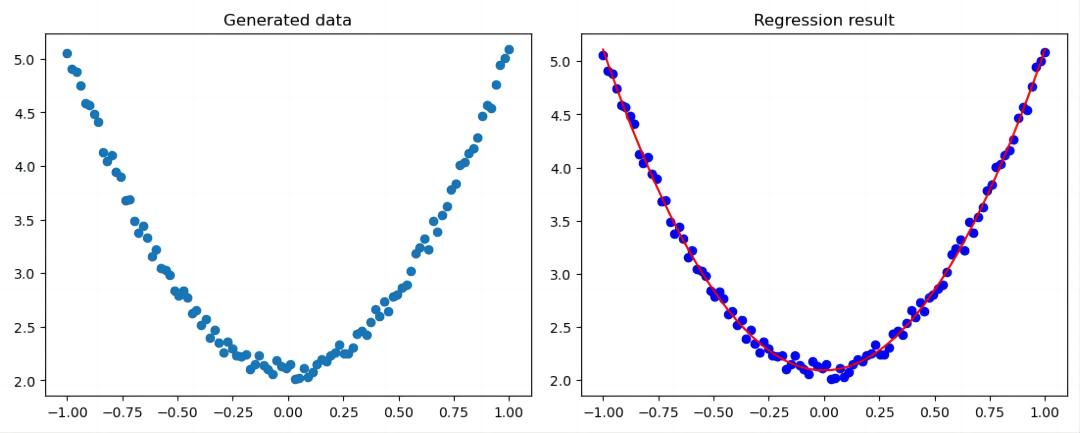
\includegraphics[width=0.8\textwidth]{part/人工智能/深度学习框架/pic/Pytorch/Pytorch基础/Numpy版实现回归问题.png}
            \caption{Numpy版实现回归问题}
            \label{fig:Numpy版实现回归问题}
    \end{figure}

    \item 使用Tensor和autograd实现
    \begin{lstlisting}[style=pythonstyle]
    # 导入所需的库
    import numpy as np
    from matplotlib import pyplot as plt

    # 生成输入数据 x 及目标数据 y
    # 设置随机种子，生成同一份数据，以便结果复现
    torch.manual_seed(985) # np.random.seed(985)
    dtype = torch.float
    # x = np.linspace(-1, 1, 100).reshape(100, 1)
    x = torch.unsqueeze(torch.linspace(-1, 1, 100), dim=1) 
    # 在第1维增加一个维度
    # 为了后面的矩阵相乘y_pred = x.pow(2).mm(w)，需要将 x 转换为矩阵形式
    #y = 3 * np.power(x, 2) + 2 + 0.2 * np.random.rand(x.size).reshape(100, 1)
    y = 3 * x.pow(2) + 2 + 0.2 * torch.rand(x.size())
    plt.title("Generated data")
    plt.scatter(x.numpy(), y.numpy()) # 画图时需要将张量转换为 numpy 数组
    plt.show()

    ################################
    # 回归模型
    # 1.初始化参数
    # w = np.random.rand(1, 1)
    w = torch.rand(1, 1, dtype=dtype, requires_grad=True)
    # b = np.random.rand(1, 1)
    b = torch.rand(1, 1, dtype=dtype, requires_grad=True)

    # 2.训练模型
    lr = 0.001  # 学习率
    epochs = 1000  # 迭代次数
    for i in range(epochs):
        # 1)前向传播
        # y_pred = np.power(x, 2).dot(w) + b
        y_pred = x.pow(2).mm(w) + b # .mm()表示矩阵相乘
        # 2)计算损失
        loss = 0.5 * (y_pred - y) ** 2
        loss = loss.sum()
        # 3)自动计算梯度
        # grad_w = np.sum((y_pred - y) * np.power(x, 2))
        # grad_b = (y_pred - y).sum()
        loss.backward()
        # 4)更新参数,使用梯度下降法使得损失函数最小
        # w -= lr * grad_w
        # b -= lr * grad_b
        with torch.no_grad(): # 不记录梯度
            w -= lr * w.grad
            b -= lr * b.grad
            # 梯度清零
            w.grad.zero_()
            b.grad.zero_()
        
        # if i % 100 == 0:
        #     print(f"Epoch {i}, Loss {loss}")
        if i % 100 == 0:
            print(f"Epoch {i}, Loss {loss.item()}")

    ################################  
    # 可视化结果
    plt.title("Regression result")
    plt.plot(x.numpy(), y_pred.detach().numpy(), 'r-', label='predict', linewidth=4) # detach() 从计算图中分离
    plt.scatter(x.numpy(), y.numpy(), color='blue', marker='o', label='true')
    plt.legend()
    plt.show()        
    \end{lstlisting}
    \begin{lstlisting}[style=demostyle,numbers=none]
    Epoch 0, Loss 431.41571044921875
    Epoch 100, Loss 2.9688427448272705
    Epoch 200, Loss 0.6887450218200684
    Epoch 300, Loss 0.2506664991378784
    Epoch 400, Loss 0.16649889945983887
    Epoch 500, Loss 0.1503276824951172
    Epoch 600, Loss 0.1472204625606537
    Epoch 700, Loss 0.14662344753742218
    Epoch 800, Loss 0.1465088278055191
    Epoch 900, Loss 0.14648674428462982
    \end{lstlisting}       
    \begin{figure}[htpb]
    \centering
    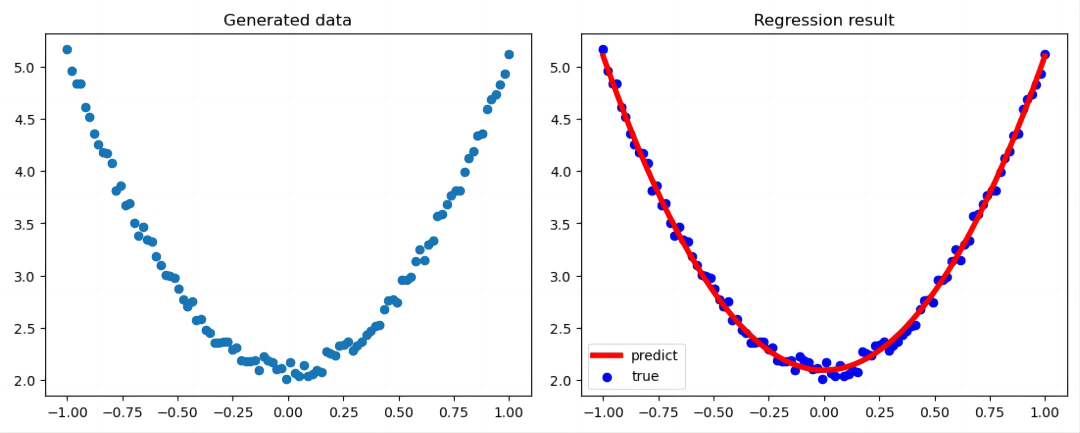
\includegraphics[width=0.8\textwidth]{part/人工智能/深度学习框架/pic/Pytorch/Pytorch基础/使用Tensor和autograd实现.png}
    \caption{使用Tensor和autograd实现}
    \label{fig:使用Tensor和autograd实现}
    \end{figure}

    如果1元2次函数使用两个参数$w_1$、$w_2$和$b$，则代码如下：
    \begin{lstlisting}[style=pythonstyle]
    # 导入所需的库
    import torch
    from matplotlib import pyplot as plt
    
    # 生成输入数据 x 及目标数据 y
    # 设置随机种子，生成同一份数据，以便结果复现
    torch.manual_seed(985)  # 设置随机种子
    
    # 使用 PyTorch 生成训练数据
    x = torch.linspace(-1, 1, 100).reshape(100, 1)  # 生成 100 个数据点
    # y = 3 * x.pow(2) + 2 + 0.2 * torch.rand(x.size())  # 生成目标数据 y
    y = 3 * x**2 + 2 + 0.2 * torch.randn(100, 1)  # 生成目标数据 y
    
    plt.title("Generated data")
    plt.scatter(x.numpy(), y.numpy())  # 画图时需要将张量转换为 numpy 数组
    plt.show()
    
    ################################
    # 回归模型
    # 1.初始化参数
    # w1 x^2 + w2 x + b
    w1 = torch.rand((1, 1), dtype=torch.float, requires_grad=True)  # 初始化权重，启用梯度
    w2 = torch.rand((1, 1), dtype=torch.float, requires_grad=True)  # 初始化权重，启用梯度
    b = torch.rand((1, 1), dtype=torch.float, requires_grad=True)  # 初始化偏置，启用梯度
    
    # 2.训练模型
    lr = 0.01  # 学习率
    epochs = 1000  # 迭代次数
    for i in range(epochs):
        # 1)前向传播
        y_pred = x.pow(2).mm(w1) + x.mm(w2) + b  # 使用 PyTorch 矩阵乘法
    
        # 2)计算损失
        loss = 0.5 * (y_pred - y).pow(2).sum()  # 使用 PyTorch 的张量操作计算损失
        # loss = (0.5 * (y_pred - y) ** 2).mean()
    
        # 3)反向传播
        loss.backward()  # 自动计算梯度
    
        # 4)更新参数,使用梯度下降法使得损失函数最小
        with torch.no_grad():
            w1 -= lr * w1.grad  # 更新权重
            w2 -= lr * w2.grad
            b -= lr * b.grad  # 更新偏置
            # 清零梯度
            w1.grad.zero_()
            w2.grad.zero_()
            b.grad.zero_()
    
        # 每100次迭代输出一次损失值
        if i % 100 == 0:
            print("epoch: {}, loss: {}".format(i, loss.item()))
            plt.scatter(x.numpy(), y.numpy())
            plt.plot(x.numpy(), y_pred.detach().numpy(), 'r-', label='predict')
            plt.title("Regression result")
            plt.legend()
            plt.show()
    
    print("w1: ", w1, "w2: ", w2, "b: ", b)
    \end{lstlisting}
    \begin{lstlisting}[style=demostyle,numbers=none]
    epoch: 0, loss: 386.6900939941406
    epoch: 100, loss: 1.4194867610931396
    epoch: 200, loss: 1.4194862842559814
    epoch: 300, loss: 1.4194862842559814
    epoch: 400, loss: 1.4194862842559814
    epoch: 500, loss: 1.4194862842559814
    epoch: 600, loss: 1.4194862842559814
    epoch: 700, loss: 1.4194862842559814
    epoch: 800, loss: 1.4194862842559814
    epoch: 900, loss: 1.4194862842559814
    w1:  tensor([[3.0083]], requires_grad=True) 
    w2:  tensor([[-0.0228]], requires_grad=True) 
    b:  tensor([[1.9803]], requires_grad=True)
    \end{lstlisting}
        
 
    \item 使用优化器及自动微分实现
    \begin{lstlisting}[style=pythonstyle]
    # 导入所需的库
    import numpy as np
    from matplotlib import pyplot as plt

    # 生成输入数据 x 及目标数据 y
    # 设置随机种子，生成同一份数据，以便结果复现
    torch.manual_seed(985) # np.random.seed(985)
    dtype = torch.float
    # x = np.linspace(-1, 1, 100).reshape(100, 1)
    x = torch.unsqueeze(torch.linspace(-1, 1, 100), dim=1) # 在第1维增加一个维度
    #y = 3 * np.power(x, 2) + 2 + 0.2 * np.random.rand(x.size).reshape(100, 1)
    y = 3 * x.pow(2) + 2 + 0.2 * torch.rand(x.size())
    plt.title("Generated data")
    plt.scatter(x.numpy(), y.numpy()) # 画图时需要将张量转换为 numpy 数组
    plt.show()

    ################################
    # 回归模型
    # 1.初始化参数
    # w = np.random.rand(1, 1)
    w = torch.rand(1, 1, dtype=dtype, requires_grad=True)
    # b = np.random.rand(1, 1)
    b = torch.rand(1, 1, dtype=dtype, requires_grad=True)

    # 2.定义损失函数和优化器
    loss_func = torch.nn.MSELoss()
    optimizer = torch.optim.SGD([w, b], lr=0.001)

    # 3.训练模型
    # lr = 0.001  # 学习率
    epochs = 1000  # 迭代次数
    for i in range(epochs):
    # 1)前向传播
    # y_pred = np.power(x, 2).dot(w) + b
    y_pred = x.pow(2).mm(w) + b # .mm()表示矩阵相乘
    loss = loss_func(y_pred, y)
    # 计算损失
    # loss = 0.5 * (y_pred - y) ** 2
    # loss = loss.sum()
    # 2)自动计算梯度
    # grad_w = np.sum((y_pred - y) * np.power(x, 2))
    # grad_b = (y_pred - y).sum()
    loss.backward()
    # 3)更新参数,使用梯度下降法使得损失函数最小
    # w -= lr * grad_w
    # b -= lr * grad_b
    # with torch.no_grad(): # 不记录梯度
    #     w -= lr * w.grad
    #     b -= lr * b.grad
    #     # 梯度清零
    #     w.grad.zero_()
    #     b.grad.zero_()
    optimizer.step()
    # 因通过autograd计算的梯度会累加到grad中，故每次循环需把梯度清零
    optimizer.zero_grad() 

    
    # if i % 100 == 0:
    #     print(f"Epoch {i}, Loss {loss}")
    if i % 100 == 0:
            print(f"Epoch {i}, Loss {loss.item()}")

    ################################  
    # 可视化结果
    plt.title("Regression result")
    plt.plot(x.numpy(), y_pred.detach().numpy(), 'r-', label='predict', linewidth=4) # detach() 从计算图中分离
    plt.scatter(x.numpy(), y.numpy(), color='blue', marker='o', label='true')
    plt.legend()
    plt.show()
    \end{lstlisting}   
    \begin{lstlisting}[style=demostyle,numbers=none] 
    Epoch 0, Loss 8.628314018249512
    Epoch 100, Loss 5.594874858856201
    Epoch 200, Loss 3.659278631210327
    Epoch 300, Loss 2.423168182373047
    Epoch 400, Loss 1.632761836051941
    Epoch 500, Loss 1.1263880729675293
    Epoch 600, Loss 0.8010491132736206
    Epoch 700, Loss 0.5911281108856201
    Epoch 800, Loss 0.4548189640045166
    Epoch 900, Loss 0.36548832058906555
    \end{lstlisting}   
    \begin{figure}[htpb]
            \centering
            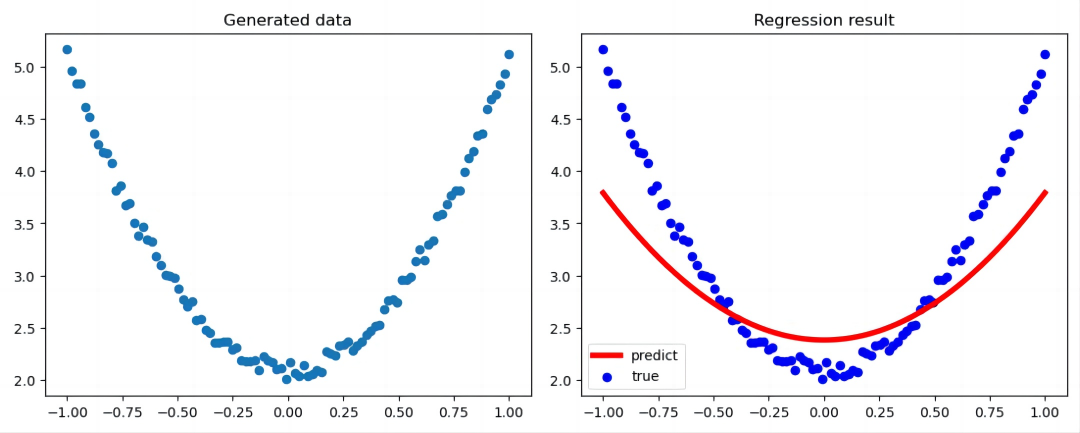
\includegraphics[width=0.8\textwidth]{part/人工智能/深度学习框架/pic/Pytorch/Pytorch基础/使用优化器及自动微分实现.png}
            \caption{使用优化器及自动微分实现}
            \label{fig:使用优化器及自动微分实现}
    \end{figure}                    

    \item 把数据集转换为带批量处理功能的迭代器
    把数据集转换为带批量处理功能的迭代器，这样训练时就可进行批量处理。
    如果数据量比较大，采用批量处理可提升训练模型的效率及性能。
    \begin{lstlisting}[style=pythonstyle]
    # 导入所需的库
    import numpy as np
    from matplotlib import pyplot as plt
    import torch

    # 生成输入数据 x 及目标数据 y
    # 设置随机种子，生成同一份数据，以便结果复现
    # np.random.seed(985)
    # x = np.linspace(-1, 1, 100).reshape(100, 1)
    # y = 3 * np.power(x, 2) + 2 + 0.2 * np.random.rand(x.size).reshape(100, 1)
    # plt.title("Generated data")
    # plt.scatter(x, y)
    # plt.show()


    ################################
    # 回归模型
    # 1.初始化参数
    # w = np.random.rand(1, 1)
    # b = np.random.rand(1, 1)
    def deta_iter(features, labels, batch_size=8):
    num_examples = len(features)
    indices = list(range(num_examples))
    # 随机读取样本，打乱顺序
    np.random.shuffle(indices)
    for i in range(0, num_examples, batch_size):
            indexs = torch.LongTensor(indices[i: min(i + batch_size, num_examples)]) # 最后一次可能不足一个batch
            yield features.index_select(0, indexs), labels.index_select(0, indexs)

    # 2.定义损失函数和优化器
    loss_func = torch.nn.MSELoss()
    optimizer = torch.optim.SGD([w, b], lr=0.001)

    # 3.训练模型
    lr = 0.001  # 学习率
    epochs = 1000  # 迭代次数
    for i in range(epochs):
    for features, labels in deta_iter(x, y, 10):
            # 1)前向传播
            y_pred = features.pow(2).mm(w) + b
            loss = loss_func(y_pred, labels)

            # 2)自动计算梯度
            loss.backward()

            # 3)更新参数,使用梯度下降法使得损失函数最小
            optimizer.step()
            optimizer.zero_grad()

    if i % 100 == 0:
            print(f"Epoch {i}, Loss {loss.item()}")
    print("w:", w, "b:", b)        

    ################################  
    # 可视化结果
    y_pred = x.pow(2).mm(w).detach().numpy() + b.detach().numpy()
    plt.title("Regression result")
    plt.plot(x.numpy(), y_pred, 'r-', label='predict', linewidth=4)
    plt.scatter(x.numpy(), y.numpy(), color='blue', marker='o', label='true')
    plt.legend()
    plt.show()
    \end{lstlisting}
    \begin{lstlisting}[style=demostyle,numbers=none]
    poch 0, Loss 0.004008688032627106
    Epoch 100, Loss 0.002615853678435087
    Epoch 200, Loss 0.002760492265224457
    Epoch 300, Loss 0.001538299024105072
    Epoch 400, Loss 0.004123619291931391
    Epoch 500, Loss 0.003147989511489868
    Epoch 600, Loss 0.0033883980941027403
    Epoch 700, Loss 0.0021358653903007507
    Epoch 800, Loss 0.004264053888618946
    Epoch 900, Loss 0.002425102051347494

    w: tensor([[3.0139]], requires_grad=True) b: tensor([[2.0920]], requires_grad=True)
    \end{lstlisting}
    \begin{figure}[htpb]
            \centering
            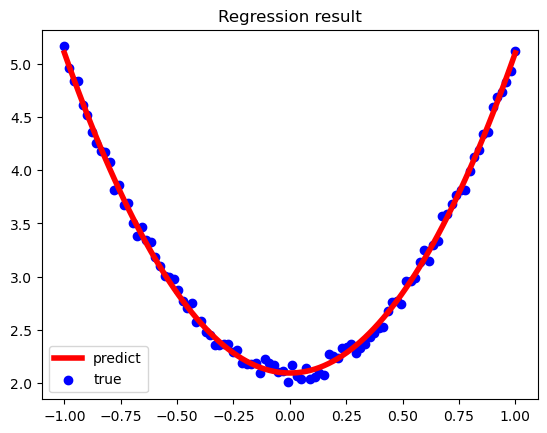
\includegraphics[width=0.8\textwidth]{part/人工智能/深度学习框架/pic/Pytorch/Pytorch基础/把数据集转换为带批量处理功能的迭代器.png}
            \caption{把数据集转换为带批量处理功能的迭代器}
            \label{fig:把数据集转换为带批量处理功能的迭代器}
    \end{figure}

\end{enumerate}

